% -*- Mode:TeX -*-

%% The documentclass options along with the pagestyle can be used to generate
%% a technical report, a draft copy, or a regular thesis.  You may need to
%% re-specify the pagestyle after you \include  cover.tex.  For more
%% information, see the first few lines of mitthesis.cls. 

%\documentclass[12pt,vi,twoside]{mitthesis}
%%
%%  If you want your thesis copyright to you instead of MIT, use the
%%  ``vi'' option, as above.
%%
%\documentclass[12pt,twoside,leftblank]{mitthesis}
%%
%% If you want blank pages before new chapters to be labelled ``This
%% Page Intentionally Left Blank'', use the ``leftblank'' option, as
%% above. 

\documentclass[12pt,twoside]{mitthesis}
\usepackage[left=1in, right=1in, top=1in, bottom=1in]{geometry} 
\usepackage{lgrind}
\usepackage{graphicx}
\usepackage{amsmath}
\usepackage{subfigure}
\usepackage[small, width = .7\textwidth, center]{caption}
\usepackage{tikz}
\usepackage{natbib}
\usepackage{bm}
\usepackage{epstopdf}
\usepackage{listings}
\usepackage{color}
\usepackage{url}
\usepackage{multirow}
\pagestyle{plain}

\definecolor{dkgreen}{rgb}{0,0.6,0}
\definecolor{gray}{rgb}{0.5,0.5,0.5}
\definecolor{mauve}{rgb}{0.58,0,0.82}

\lstset{frame=tb,
  language=Java,
  aboveskip=3mm,
  belowskip=3mm,
  showstringspaces=false,
  columns=flexible,
  basicstyle={\small\ttfamily},
  numbers=none,
  numberstyle=\tiny\color{gray},
  keywordstyle=\color{blue},
  commentstyle=\color{dkgreen},
  stringstyle=\color{mauve},
  breaklines=true,
  breakatwhitespace=true
  tabsize=2
}

%% This bit allows you to either specify only the files which you wish to
%% process, or `all' to process all files which you \include.
%% Krishna Sethuraman (1990).

%\typein [\files]{Enter file names to process, (chap1,chap2 ...), or `all' toprocess all files:}
%\def\all{all}
%\ifx\files\all \typeout{Including all files.} \else \typeout{Including only \files.} \includeonly{\files} \fi
\newcommand{\superscript}[1]{\ensuremath{^{\textrm{#1}}}}
\newcommand{\subscript}[1]{\ensuremath{_{\textrm{#1}}}}
\newcommand{\eqdef}{\overset{\mathrm{def}}{=\joinrel=}}

\makeatletter
\providecommand*{\diff}%
{\@ifnextchar^{\DIfF}{\DIfF^{}}}
\def\DIfF^#1{%
\mathop{\mathrm{\mathstrut d}}%
\nolimits^{#1}\gobblespace}
\def\gobblespace{%
\futurelet\diffarg\opspace}
\def\opspace{%
\let\DiffSpace\!%
\ifx\diffarg(%
\let\DiffSpace\relax
\else
\ifx\diffarg[%
\let\DiffSpace\relax
\else
\ifx\diffarg\{%
\let\DiffSpace\relax
\fi\fi\fi\DiffSpace}

\begin{document}

% -*-latex-*-
% 
% For questions, comments, concerns or complaints:
% thesis@mit.edu
% 
%
% $Log: cover.tex,v $
% Revision 1.8  2008/05/13 15:02:15  jdreed
% Degree month is June, not May.  Added note about prevdegrees.
% Arthur Smith's title updated
%
% Revision 1.7  2001/02/08 18:53:16  boojum
% changed some \newpages to \cleardoublepages
%
% Revision 1.6  1999/10/21 14:49:31  boojum
% changed comment referring to documentstyle
%
% Revision 1.5  1999/10/21 14:39:04  boojum
% *** empty log message ***
%
% Revision 1.4  1997/04/18  17:54:10  othomas
% added page numbers on abstract and cover, and made 1 abstract
% page the default rather than 2.  (anne hunter tells me this
% is the new institute standard.)
%
% Revision 1.4  1997/04/18  17:54:10  othomas
% added page numbers on abstract and cover, and made 1 abstract
% page the default rather than 2.  (anne hunter tells me this
% is the new institute standard.)
%
% Revision 1.3  93/05/17  17:06:29  starflt
% Added acknowledgements section (suggested by tompalka)
% 
% Revision 1.2  92/04/22  13:13:13  epeisach
% Fixes for 1991 course 6 requirements
% Phrase "and to grant others the right to do so" has been added to 
% permission clause
% Second copy of abstract is not counted as separate pages so numbering works
% out
% 
% Revision 1.1  92/04/22  13:08:20  epeisach

% NOTE:
% These templates make an effort to conform to the MIT Thesis specifications,
% however the specifications can change.  We recommend that you verify the
% layout of your title page with your thesis advisor and/or the MIT 
% Libraries before printing your final copy.
\title{Real-time Continuous Gesture Recognition for Natural Multimodal Human
Computer Interaction}

\author{Ying Yin}
% If you wish to list your previous degrees on the cover page, use the 
% previous degrees command:
%       \prevdegrees{A.A., Harvard University (1985)}
% You can use the \\ command to list multiple previous degrees
%       \prevdegrees{B.S., University of California (1978) \\
%                    S.M., Massachusetts Institute of Technology (1981)}
\department{Department of Electrical Engineering and Computer Science}

% If the thesis is for two degrees simultaneously, list them both
% separated by \and like this:
\degree{Doctor of Philosophy}
%\degree{Bachelor of Science in Computer Science and Engineering}

% As of the 2007-08 academic year, valid degree months are September, 
% February, or June.  The default is June.
\degreemonth{June}
\degreeyear{2014}
\thesisdate{May 18, 2014}

%% By default, the thesis will be copyrighted to MIT.  If you need to copyright
%% the thesis to yourself, just specify the `vi' documentclass option.  If for
%% some reason you want to exactly specify the copyright notice text, you can
%% use the \copyrightnoticetext command.  
%\copyrightnoticetext{\copyright IBM, 1990.  Do not open till Xmas.}

% If there is more than one supervisor, use the \supervisor command
% once for each.
\supervisor{Randall Davis}{Professor}

% This is the department committee chairman, not the thesis committee
% chairman.  You should replace this with your Department's Committee
% Chairman.
\chairman{Arthur C. Smith}{Chairman, Department Committee on Graduate Theses}

% Make the titlepage based on the above information.  If you need
% something special and can't use the standard form, you can specify
% the exact text of the titlepage yourself.  Put it in a titlepage
% environment and leave blank lines where you want vertical space.
% The spaces will be adjusted to fill the entire page.  The dotted
% lines for the signatures are made with the \signature command.
\maketitle

% The abstractpage environment sets up everything on the page except
% the text itself.  The title and other header material are put at the
% top of the page, and the supervisors are listed at the bottom.  A
% new page is begun both before and after.  Of course, an abstract may
% be more than one page itself.  If you need more control over the
% format of the page, you can use the abstract environment, which puts
% the word "Abstract" at the beginning and single spaces its text.

%% You can either \input (*not* \include) your abstract file, or you can put
%% the text of the abstract directly between the \begin{abstractpage} and
%% \end{abstractpage} commands.

% First copy: start a new page, and save the page number.
\cleardoublepage
% Uncomment the next line if you do NOT want a page number on your
% abstract and acknowledgments pages.
% \pagestyle{empty}
\setcounter{savepage}{\thepage}
\begin{abstractpage}
I have developed a real-time continuous gesture recognition system capable of
dealing with two important problems that have previously been neglected:
(a) smoothly handling two different kinds of gestures: those
characterized by distinct paths and those characterized by distinct hand
poses; and (b) determining how and when the system should respond to gestures
The novel approaches in this thesis include: a probabilistic recognition
framework based on a flattened hierarchical hidden Markov model (HHMM) that
unifies the recognition of path and pose gestures;
and a method of using information from the
hidden states in the HMM to identify different
gesture phases (the pre-stroke, the nucleus and the post-stroke
phases), allowing the system to respond appropriately to both gestures that
require a discrete response and those needing a continuous response.

The system is extensible: new gestures can be added by recording 3-6 repetitions
of the gesture; the system will train an HMM model for the gesture
and integrate it into the existing HMM, in a process that takes only a few minutes.
Our evaluation shows that even using only a small number of
training examples (e.g. 6), the system can achieve an average $F_1$ score of
0.805 for
two forms of gestures.

To evaluate the performance of my system I collected a new dataset
(YANG dataset) that includes both path and pose gestures, offering a
combination currently lacking in the community and providing
the challenge of recognizing different types of gestures mixed
together. I also developed a novel hybrid evaluation metric that is
more relevant to real-time interaction with different gesture flows.
\end{abstractpage}

% Additional copy: start a new page, and reset the page number.  This way,
% the second copy of the abstract is not counted as separate pages.
% Uncomment the next 6 lines if you need two copies of the abstract
% page.
% \setcounter{page}{\thesavepage}
% \begin{abstractpage}
% I have developed a real-time continuous gesture recognition system capable of
dealing with two important problems that have previously been neglected:
(a) smoothly handling two different kinds of gestures: those
characterized by distinct paths and those characterized by distinct hand
poses; and (b) determining how and when the system should respond to gestures
The novel approaches in this thesis include: a probabilistic recognition
framework based on a flattened hierarchical hidden Markov model (HHMM) that
unifies the recognition of path and pose gestures;
and a method of using information from the
hidden states in the HMM to identify different
gesture phases (the pre-stroke, the nucleus and the post-stroke
phases), allowing the system to respond appropriately to both gestures that
require a discrete response and those needing a continuous response.

The system is extensible: new gestures can be added by recording 3-6 repetitions
of the gesture; the system will train an HMM model for the gesture
and integrate it into the existing HMM, in a process that takes only a few minutes.
Our evaluation shows that even using only a small number of
training examples (e.g. 6), the system can achieve an average $F_1$ score of
0.805 for
two forms of gestures.

To evaluate the performance of my system I collected a new dataset
(YANG dataset) that includes both path and pose gestures, offering a
combination currently lacking in the community and providing
the challenge of recognizing different types of gestures mixed
together. I also developed a novel hybrid evaluation metric that is
more relevant to real-time interaction with different gesture flows.
% \end{abstractpage}

\cleardoublepage

\section*{Acknowledgments}

This is the acknowledgements section.  You should replace this with your
own acknowledgements.

%%%%%%%%%%%%%%%%%%%%%%%%%%%%%%%%%%%%%%%%%%%%%%%%%%%%%%%%%%%%%%%%%%%%%%
% -*-latex-*-

\pagestyle{plain}
\tableofcontents
\listoffigures
\listoftables
\section{Introduction}
\begin{quotation}
\textit{Imagine an earthquake has hit a populous area and many major roads are
impassable. Buildings are serverly damaged or collapsed, and fire has broken out
in many places. At the crisis management center, response professionals are
working together to coordinate the earthquake releif effort. You are the
incident commander charged with coordinating the search
and rescue teams working in the field.}

\textit{A report about a big explosion at a chemical plant comes in and you move
the map around, zoom in and rotate it to get a good view of the site. On the map, you
see there is a group of unmanned vehicles nearby and you select them on
the map using your hand and instruct them to go nearer to the explosion site to
gather more information by tracing the route they should take to avoid obstacles. 
Then you instruct rescue team No. 3 to evacuate the residents
in the sorrounding buildings by going under a bridge because the surface of the
bridge is block. You gesture with one hand as the bridge and the other
hand moving under it to emphasize this.}
\end{quotation}

The scenario above shows an application of a multi-modal interface to a
real-world problem. Gestures play an important part in this scenario,
providing key information about location, method adn timing of movement,
and about spatial relationship among the objects being described.

Recent trends in user interfaces have brought on a new wave of interaction
techniques that depart from the traditional mouse and keyboard that have been used for decades. These include multi-touch interfaces such as the iPhone\textsuperscript{\textregistered}, iPad and the Microsoft Surface\textsuperscript{\textregistered} as well as camera-based systems such as the Nintendo\textsuperscript{\textregistered} Wii and the Microsoft Kinect. Most of these devices gained instant popularity among consumers, and the common trait among them is that they make interacting with computation more natural and effortless. All these devices allow users to use their hands and/or body
gestures to directly manipulate the virtual objects. It feels more natural this
way because this is how we interact with our environment in everyday
life.
 
Our goal is to take this aspiration to the next level by developing an
intelligent multimodal interface for natural interaction. By \textit{natural
interaction}, we mean the kind of cognitively transparent, effortless multimodal
communication that can happen between people; we want to make this possible in
human-computer interaction such that the computer interface understands what the
user is saying and doing, and the user can simply behave. We believe that
natural interaction can provide better learnability, flexibility, memorability,
convenience and efficiency, but further user studies are needed to investigate
this belief.

Gesture plays an important part in multimodal interaction, especially for
conveying spatial information. The focus of this thesis is developing a
hierarchical approach for continous gesture analysis that can be easily
applied in different domains and applications. Specifically we focus on gestures
made with hands.

\section{Previous Work}
The current state of art of hand-based gesture interfaces involves tracking
hands as blobs or fingertips as points, and recognizing a set of
predefined gestures suited to the tasks involved in the applications
either based on heuristics or feature-based models.

Bolt's pioneering work in the ``Put That There'' system \cite{Bolt80} demonstrated the potential for voice and gestural interaction.  In that system, the hand position and orientation was tracked by the Polhemus tracker, i.e., the hand was essentially transformed to a point on the screening. The actual hand posture did not matter, even if it was not in a pointing shape. The speech also followed a rigid and limited command-like grammar. Even though this is an early work, it provides some insight about the advantages of multimodal interaction. As Bolt summarized in the paper, using pointing gesture allows the use of pronouns in the speech, with the corresponding gain in naturalness and economy of expression \cite{Bolt80}. 

Multi-touch displays have gained significant media attention and popularity with the introduction of iPhone\textsuperscript{\textregistered} and Microsoft Surface\textsuperscript{\textregistered}. Their wide popularity shows the great potential and demand for natural and convenient input techniques. However, with touch-based input, the interaction is still limited in 2D space, and some 3D interaction cannot be realized, or is hard and unnatural to specify. For instance, it will be hard to rotate a map in 3D with a touch-based display. In addition, these new interfaces are more like a replacement for mouse input, with the addition of processing multiple input points at the same time. 

(Mention iPad, tablets, Kinect)

Moving from 2D to 3D, Oblong Industries' g-speak spatial operating environment addresses the constriction of human intent imposed by traditional GUIs \cite{Oblong09}. The g-speak platform braids development arcs begun in the early 1990s at MIT's Media Laboratory, allowing free hand input in 3D space. However, it focuses only on using hand for manipulating pixels, instead of going beyond to exploit the communicative power of gesture. 

The introduction of Nintendo Wii is a break-through in interaction techniques for the gaming industry. Its success once again indicates people's preference for natural interaction that is similar to what we do in the real world. At Electronic Entertainment Expo 2009 Microsoft unveiled its Project Natal which is a controller-free gaming and entertainment system. It enables user to play video games through a natural user interface using gestures and spoken commands. The device provides full-body 3D motion capture. However, it does not track the hand posture at a finer level. Some of the features of Project Natal are still concepts, but it does paint an exciting future for natural human-computer interaction, such as the user can have a natural conversation with the animated character in the game.

In the research community, several multi-modal interaction prototypes were developed that moved beyond Bolt's ``Put That There'' system. Cohen et al. \cite{Cohen97} developed the QuickSet prototype which is a collaborative, multimodal system running on a hand-held PC using pen and voice as input. They used a novel multimodal integration strategy that allows speech and pen gesture to compensate for each other, yielding a more robust system. Rauschert et al. \cite{Rauschert02} developed a system called Dialogue-Assisted Visual Environment for Geoinformation (DAVE\_G) that uses free hand gestures and speech as input. They recognized that gestures are more useful for expressing spatial relations and locations. Gestures in DAVE\_G included pointing, indicating an area and outlining contours. Speech and gesture are fused for commands that need spatial information provided by the gesture. Their work, however, mainly tracked hand location, rather than tracking both location and posture, as in our work.

\section{Proposed Work and Procedure}\
Our motivation is to build a computer system that can understand the natural
gestures made by people (sometimes called gesticulation) without restrcting the
gesturers to a narrow set of predefined motions and hand configurations.

\subsection{Gestural Taxonomy}

\subsection{Project Setup}
The custom tabletop structure includes four $1280\times1024$ pixel projectors (Dell 5100MP) that provide a $2560\times2048$ pixel resolution. The projectors are connected to two NVIDIA GeForce 8600GT dual-headed graphics card on a Dual-Core 2.4GHz desktop PC with 2GB of RAM.

\begin{figure}
	\centering
	\includegraphics[width=0.7\textwidth]{figures/setup.png} 
	\caption{System setup.} \label{fig:setup}
\end{figure}

The display is projected onto a flat white surface digitizer (GTCO Calcomp DrawingBoard V), which uses a stylus as an input device. The digitizer is tilted 10 degrees down in front, and is placed at 41in (104cm) above the floor, following FAA's design standard to accommodate the $5^{th}$ through $95^{th}$ percentiles of population. Projected displays were mechanically aligned to produce a single seamless large display area. One Fire-i\texttrademark Digital Camera from Unibrain is placed above the center of the tabletop at the same level of the projectors. We use the Google Earth web browser plug-in as our basis for 3D maps. Figure \ref{fig:setup} shows the setup.

The Dell 5100MP projector uses a spinning color wheel to modulate the image. This produces a visible artifact on the screen, referred to as the ``rainbow effect'', with colors separating out in distinct red, green, and blue. At any given instant in time, the image on the screen is either red, or green, or blue, and the technology relies upon people's eyes not being able to detect the rapid changes from one to the other. However, when seen through a camera, the effect is very obvious, and this can greatly affect the color classification for the hand tracking. To reduce this effect, the exposure rate of the camera needs to be adjusted to be a multiple of the rotation period of the color wheel. The projector uses 2x color wheel speed, which is about 120 rotation/second. Hence, the period is about 8.3ms. After adjusting the exposure rate of the camera to approximately 8.3ms, the effect is greatly mitigated, but still present. 

\subsection{Hand Tracking}
An important part of multimodal interface is acquiring valid multimodal data. The most common acquisition methods for hand gestures are magnetic trackers, cyber-gloves and vision-based approaches. Acquisition using magnetic trackers and cybergloves is efficient and accurate, but suffers from the need to wear restrictive devices. Most existing vision-based hand tracking systems track only hand movement and finger tips, rather than 3D hand posture \cite{Demirdjian03}\cite{Oka02}\cite{Rauschert02}. This limitation often requires that artificial gestures be defined for easy tracking and recognition.  

\begin{figure}
	\centering
	\includegraphics[width=0.6\textwidth]{figures/tabletop.png} 
	\caption{Hand tracking with a colored glove.} \label{fig:tabletop}
\end{figure}

We use the hand-tracking system developed by Robert Y. Wang \cite{Wang09}. With one web camera and one ordinary cloth glove imprinted with a custom pattern (see Figure ~\ref{fig:tabletop}), the system can track 3D hand posture in real-time. It provides rich hand model data with 26 degree of freedoms (DOFs): six DOFs for the global transformation and four DOFs per finger. The glove is very light-weight, with no additional electronics and wires. As a result, the hand gestures we can use for interaction will not be limited by the hand-tracking hardware, opening up possibilities for developing and investigating more natural gestural interaction.

We use a different web camera from the one used by Wang. This is also a verification that the hand-tracking system is compatible and works well with different ordinary webcams. Using the FireAPI\texttrademark 1394a/1394b development toolkit, we developed a wrapper for the Fire-i camera driver to interface with the hand-tracking system. The camera is set to capture $640 \times 480$ video at 15Hz.  

Wang's hand-tracking software was developed originally for use in an office environment with standard illumination. Several interesting steps are required to use it in our context, with its complex and dynamic background (the maps) and the non-uniform illumination of the glove from the maps. 

To eliminate the effect of the background, the image captured by camera is divided by the background image. Traditional background subtraction involves taking a static image of the background or keeping a running average of the images as the background, and then subtracting the background image from the current image. The problem is slightly different in our case as the background is the display, and we know what is been displayed by taking a screen capture. We then apply geometric and color transformations to the screen capture to dynamically compute the background image as it is seen by the camera. Figure \ref{fig:transImgPxl} shows how the image pixels from the computer graphics card are transformed as they are projected to the tabletop and then captured by the camera (Step 1-4). Image A is the camera captured image. Image B is the background we want to compute so that we can eliminate the background from Image A. Step 5 is the process where we take Image C directly from the graphics card through screen capture and transform (scaling, cropping, and color mapping) it to Image B.

\begin{figure}
	\centering
	\includegraphics[width=0.8\textwidth]{figures/transImgPxl.png} 
	\caption{Transformation of image pixels.} \label{fig:transImgPxl}
\end{figure}

As the projectors are above the table, the light from the project is also shone on the hand. The color signal reaching the camera is the multiplication of illumination and reflectance of the color glove for each pixel. To eliminate the effect of the illumination on the glove, we first rectify the camera image (removing distortion in Image A), and then divide the camera image RGB values term-by-term by the screen capture values after color transformation (Image B). Figure \ref{fig:divided} shows an example of the result after division where the background is mostly white and the glove colors are closer to the actual colors. The result is not perfect either due to the imperfection in the geometric and color calibrations, however, color classification of the glove colors based on the image after background elimination is more robust.

\begin{figure}
	\centering
	\includegraphics[width=0.6\textwidth]{figures/divided.png} 
	\caption{Transformation of image pixels.} \label{fig:divided}
\end{figure}

The above method relies on correctly capturing the display through screen capture. As the user interacts with the interface, the display changes, and hence we need to recapture the background. There are two approaches: one is having a thread continuously taking screen capture; the other is only taking the screen capture when the background changes. Obviously, the second approach is more computationally efficient, however it also relies more on capturing the background at the correct moment. We will experiment with both methods or use a combination of the two approaches.

We will also try another background subtraction method by using polarizing filters. We will cover the surface of the tabletop with a sheet of polarizing filter, and put another filter in front of the camera lens such that the axes of light transmission of the two filters are orthogonal to each other. In this way the background will be completely black.
   
\subsection{Gesture Recognition}
We adopt the taxonomy of hand movements proposed by Pavlovi\'{c} et al. \cite{Pavlovic97} which distinguishes gestures from unintentional hand movements (like beats). They then further divided the gestures into manipulative and communicative classes. 

Many previous systems distinguish gestures from unintentional hand movements by restricting the hand motion or defining some arbitrary gesture to indicate the start of gesture \cite{Shin04}. With the ability to track 3D hand postures in real-time, we can train the gesture recognizer with a set of natural gestures without being worried about whether those gestures are easily recognized by the system. Any hand motion that is not classified will not have a effect on the state of the system.

Manipulative gestures are the ones used to act on objects, while communicative ones have an inherent communicational purpose\cite{Pavlovic97}. In a natural environment, communicative gestures are usually accompanied by speech. Hence, for manipulative gestures, our classification will be entirely based on the hand states, while for communicative gestures, both hand and speech recognitions will be combined for recognition. 

The output from the hand tracker is a sequence of data describing the translation (in x, y, z coordinates) and orientation (in a quaternion) of the hand and each finger joint. There are three joints per finger in the model. The joint at the base of each finger has 2 DOFs while the other two joints of each finger have 1 DOF each. From the tracker output, we derive the feature vector at each time frame. For each finger, we are interested in the bending angles of the joints. Hence, we convert the joint orientation in quaternion to Euler angles. The translation of the joint is irrelevant because it is relative to the hand and stays the same. The feature vector includes the speed of hand movement in the x-y plane (obtained from the global translation of the hand), z position of the hand, roll, pitch and yaw of the hand, and four angles for each finger (one angle for each of the first two joints and two angles for the base joint). The result is a 25-dimensional feature vector.

\begin{figure}[htp]
\begin{center}
\includegraphics[width=.7\textwidth]{figures/Bakis.jpg}
\caption{{The state transition diagram of a 4-state Bakis model with corresponding transition probabilities}}\label{fig:bakis}
\end{center}
\end{figure}

The position and the orientation of the hand through time can be assumed to follow the first order Markov process \cite{Starner95}. Hence, we use Hidden Markov Models (HMMs) to classify gestures. There exist many kinds of HMMs \cite{Rabiner86}. One that can model time-series signals whose characteristics change successively over time is called the Bakis model \cite{Bauer00} or the Left-Right model \cite{Rabiner90}, often used in speech recognition systems \cite{Bauer00}. The Bakis model allows transitions to the same state, the next state, and the one after the next state.  Figure \ref{fig:bakis} shows an example of the Bakis model with 4 states. The Bakis model topology is particularly useful for our task because it allows different gesture speeds to be compensated \cite{Bauer00}.
	
In our experiments, we used a 6-state Bakis model, and obtained training data for 11 gestures (including panning left, right and up; roll, pitch and yaw in clockwise and anticlockwise directions, and zoom in and out). There is one HMM trained for each gesture. The probability of an observed sequence is evaluated for all competing models, and the classification is based on the model that gives the highest log-likelihood. To date, we have achieved 95\% accuracy for isolated gesture recognition. 

The next important step is continuous online gesture recognition. One issue is segmenting the continuous hand movement to get gesture intervals. The HMMs are trained for isolated gestures. When these gestures are connected together, in between, there may be unintentional hand movements, the hand may be at rest, or out of the scene. We need to add these considerations into our model.

Another issue is achieving minimum time delay of gesture recognition for a real-time interactive system. Such performance is difficult to achieve because that the starting and ending points of the gesture are not known. We will use a dynamic threshold to prune the competing gesture models based on their relative log-likelihood values. In this way, we can narrow down on a particular gesture even before the gesture ends. We will experiment with different ways of computing the dynamic threshold through data analysis of training data and cross-validation.
 
\subsection{Communicative Gesture and Speech Recognition} 
For this study, we will focus more on gesture recognition and interaction. However, as communicative gestures often co-occur with speech, we may add some basic speech recognition capability to the system in order to combine speech and deictic gestures for some USAR interaction scenarios.

\subsection{Interface with Google Earth}
Using the Google Earth Plug-in and its JavaScript API,  we embedded Google Earth, a 3D digital globe, into a web page. We use the Java web browser object in the JDesktop Integration Components (JDIC) library to load the webpage. In this way, we can augment the browser and make it respond to the gesture events from the gesture recognizer and provide the corresponding actions on the map. 

\subsection{User Study}\label{sec:userStudy}
In order to develop an interface for natural interaction in USAR Command and Control, we need to first understand what kinds of spontaneous speech, drawings, and gestures people make in such scenarios. We will try to answer this question by conducting a user study under an incident command system (ICS) environment with our tabletop display system. Experimental subjects will play the role of command center personnel charged with receiving event reports coming in from the field, making appropriate updates to a map display, then communicating commands to personnel in the field. As the user study is for bootstrapping an experimental testbed, we want minimum overhead in terms of system development. Hence, no attempt will be made in this exercise to process the drawings, speech or gestures. Instead, we will videotape the subjects and record the annotations they draw, then analyze the results to find commonalities. 

\section{Schedule}
\begin{enumerate}
	\item Experiment with polarizing filters \hfill Done by Jan 31, 2010
	
	Test whether using polarizing filters can provide better result than computing the background, or maybe we can use both methods.
	
	\item Continuous online gesture recognition \hfill Done by Feb 14, 2010
	
	Improve algorithms on continuous online gesture recognition. Conduct quantitative evaluation of the recognition results. 
	
	\item Connect user interface with gesture recognition	\hfill Done by Feb 28, 2010
	
	Interface with Google Earth. Improve system response time with gesture interaction. May need to switch to more rudimentary map interface if speed is an issue for Google Earth. May add basic speech recognition.
	 
	\item User study \hfill Done by Mar 21, 2010
	
	Conduct user study described in Section \ref{sec:userStudy}.
	
	\item Write first draft of thesis report \hfill Done by Apr 15, 2010
	\item Complete thesis report	\hfill Done by Apr 30, 2010
	\end{enumerate}
	
\section{Principal Equipment and Facilities}
Here is a list of equipment and facilities needed for the study:

\begin{enumerate}
	\item A white surface digitizer (GTCO Calcomp DrawingBoard V)
	\item Four $1280\times1024$ pixel projectors (Dell 5100MP)
	\item One web camera
	\item Polarizing filters
\end{enumerate}

All the above equipment are avalaible.


\chapter{Related Work}
There is a large body of active research on using the hand as an input modality
for human-computer interaction. To do this, the computer needs to be able to
interpret the dynamic and/or static configurations of the human hand, arm, and
even other parts of the human body. We break down the gestural input
system into several sequential modules shown in Figure \ref{fig:pipeline}.

\begin{figure}[h]
  \centering
  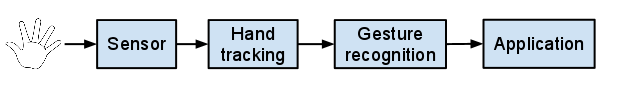
\includegraphics[width=0.7\textwidth]{figures/pipeline.png} 
  \caption{Gestural input pipeline.}
  \label{fig:pipeline}
\end{figure}

\section{Sensors}
The first step in the pipeline is having sensors that capture the hand movements
and configurations, converting analog signals to digital signals. First attempts
to solve this problem resulted in mechanical devices that directly measure hand
joint angles and spatial positions. This group is best represented by the
glove-based approaches using devices such us CyberGloves \cite{fels09} and
Powergloves \cite{kadous02}. However, wearing gloves makes gesturing more
cumbersome, and many efforts have been made to make the gloves more
light-weight, for example, by using Bluetooth wireless data transmission (e.g.,
CyberGove II). To further reduce the bulkiness of the gloves, people use colored
markers on the fingers \cite{mistry09} or colored gloves with no electronics \cite{Wang09}, and use RGB
cameras and computer vision techniques to interpret gestures. However, by
requiring the user to wear something extra still hinders the acceptance of
such devices as ``everyday'' natural interaction interfaces. 

The most non-obtrusive way to capture the hand is bare-hand tracking. Shin et
al. \cite{Shin04} use stereo RGB cameras to extract the hand from background based on the skin color. One
limitation of RGB cameras is that they are very sensitive to lighting
conditions. This prompted researchers to look into other types of cameras. Oka et al. 
\cite{Oka02} use thermal imaging for hand segmentation under complex
background and changing light, relying on the condition that a hand's
temperature is almost always distinct from the background. Their approach does
not detect finger contact with the surface. Larson et al. \cite{larson11}
improve on this method to detect the finger contact by using
the heat transferred from a user's hand to the surface for touch-based gestures.
However, in order to detect the heat trace, the user has to drag the fingers a
bit instead of just touching. This may be a small departure from what users
would expect as ``natural'' based on their experience in the physical world.

Thermal imaging measures radiation emitted by objects in the
\textit{far}-infrared (F-IR) spectrum. There are other well-known ``IR-imaging''
techniques used in the HCI community which use devices that operate in the \textit{near}-infrared (N-IR) spectrum.
N-IR is employed in some fairly recent interactive tabletop surfaces and depth
cameras. A number of projects in the HCI community have used IR for tabletop
interaction by detecting multi-touch gestures using an under mounted
camera and an illumination source. An example of this is Microsoft's 
Surface\textsuperscript{\textregistered}. Recently, portable multi-touch devices
such as phones and tablets have become more and more ubiquitous. These devices
are based on capacitive touch sensitive screens. Touch-based devices are
becoming more and more mature, however the kind of gestures one can use are still
limited. The gestures are usually limited in 2D space with one or multiple
fingers. 

Going beyond the limitation of touch-only gestures, researchers at Microsoft
augmented the Surface technology with a switchable diffuser, additional
strips of IR LEDS with a different wave length for diffuse illumination, and an
additional IR sensitive camera which images IR reflected from the diffuse
illumination of the environment \cite{hilliges09}. In this way, they can capture
the hand above the surface as well. The height of the hand is estimated based on
the pixel intensity.

Since the introduction of Kinect, a motion sensing input device by Microsoft for
the Xbox 360 video game console, researchers in the HCI community, as well as
many independent hackers, have been using Kinect's depth sensor for capturing
both body and hand gestures \cite{openni}. Since then, there are also many
similar devices coming into the market which have been used for capturing
gestures. For instance, Harrison et al. \cite{harrison11} use  a short-range
PrimeSense \cite{primesense} depth camera for their wearable multi-touch
interaction. In comparison to the aforementioned augmented Surface setup,
Kinect, and the likes, provide a cheap alternative for depth sensing. In this
thesis, we will explore the potential of using the Kinect sensor for detecting 
both the touch-based gesture and above-surface 3D gestures. Potentially, we can 
use the depth information for determining surface touch, and hence, eliminate
the need for the complicated electronics of a touch sensitive screen. This also 
enables the gestural interaction on a large tabletop display, much bigger than 
that of Microsoft's Surface.

\section{Hand Tracking}
After getting input from the sensor(s), the next step in the pipeline is
tracking the hand(s). This is essentially the frame-by-frame estimation of the
parameters of the hand model based on the sensor input. The complexity of the
hand model is application dependent. For a given application, a very coarse and
simple model may be sufficient. The simplest model is treating the hand as a
blob and only the 2D/3D location of the blob is tracked. For example, Sharma et
al. \cite{sharma00} use 2D positional and time differential parameters to track
the hands as blobs, which is sufficient for them to distinguish whether the
hands are doing a point, a contour, or a circle gesture. The PrimeSense NITE
middleware for OpenNI's natural interaction framework also tracks the hand as a
point. It requires the user to do a ``focus'' gesture (``click'' or ``wave'')
to gain control in order to start hand tracking \cite{primesense-manual}. The
gestures it supports are ``click'', ``wave'', ``swipe left'', ``swipe right'', 
``raise hand candidate'' and ``hand candidate moved''.

However, to make a more generalizable system for natural-like interaction, a
more sophisticated model is required. One step forward is adding fingertip
locations in the hand model as exemplified in \cite{Oka02} \cite{harrison11}
\cite{larson11}. Tracking fingertips is usually sufficient for manipulating
objects on the 2D surface. However, for a more rich set of gestures, the one
that also involves communicative gestures, we may need a more sophisticated
model. For instance, Wang et al. \cite{Wang09} uses a 26 DOF
3D skeletal model in their real-time hand-tracking system. 

Another approach is using an appearance-based model. This means that the model
parameters are not directly derived from the 3D spatial description of the hand.
The hand poses are modeled by relating the appearance of any pose to the 
appearance of the set of predefined, template poses \cite{Pavlovic97}. In
their markless hand-tracking system, Wang et al. \cite{wang11} use efficient
queries of a database of gestures and desktop-specific hand silhouette samples
for pinch/click gesture detection.

In our system, we propose a combination of both approaches. A simplified 3-D
skeletal hand model is useful for manipulative gestures because we want to know 
exactly where the fingertips are and the grabbing and releasing poses of the hand. For
communicative gestures, we just need to know the meaning of the gesture instead
of the exact spatial parameters. Hence example-based template models would be
more suitable which also require less computation.

\subsection{Gesture Spotting}
To distinguish unintentional movements from intentional
movements, a common approach is to use one or two nongesture HMMs to
provide likelihood thresholds for outlier rejection. For instance, in \cite{yang07}, a weak
universal movement model has been used for adaptive thresholding.
Peng et al. \cite{peng11} argue that using one or two HMMs cannot
effectively reject complex outliers, e.g., when they resemble portions of a
gesture. In addition to a general garbage gesture model, they train several
nongesture HMM models by automatically identifying and manually specifying nongesture models from the
training data. This approach is suitable when identifying dynamic communicative
gestures and when the set of the input data is limited. They only test on the
given dataset, but in real life the possible unintentional movements are
limitless and it is not clear how this approach will scale. In addition,
using nongesture HMMs only works for discrete communicative gestures, but not
for static or continuous manipulative gestures.

We will investigate the distinctions between unintentional and
intentional hand movements based on hand and arm poses and movements, and the
context of the interaction. The context of the interaction refers to the states
of the application, for examples, whether the user's hand is close to a movable
virtual object, or whether an object is selected and waits for further commands.

\section{Gesture Recognition}
Most gestural input applications have focused on tracking only
\cite{harrison11} \cite{larson11}. For hand gesture recognition, much of the
work is on synthetic gestures, most notably sign language recognition
\cite{Starner95} \cite{Bauer00} \cite{kadous02} \cite{Wang09}. For dynamic
gesture recognition, hidden Markov model (HMM) is a commonly used technique because it is suitable
for time series data \cite{sharma00}.

Elaborate more on \cite{Starner95}: embeded training: trains the models
\textit{in situ} and allows the boundaries to shift through a probabilistic
entry into the initial states of each model \cite{young1994}.

Wang et al. \cite{wang06} argue that a significant limitation of the
HMM is the requirement of conditional independence of observations. In
addition, HMM, as a generative model, optimizes the likelihood of
generating all the examples of a given gesture class, which is not
necessarily optimal for discriminating the gesture class against other
gestures. They introduced the use of hidden conditional random fields (HCRF),
an extension of conditional random fields (CRF), for gesture recognition, and
showed improved accuracy for the set of head and arm gestures they use in comparison to using HMMs. 
However, this approach does not handle continuous input. 

Morency et al. \cite{morency07} present a latent-dynamic conditional
random field (LDCRF) model that is able to perform sequence labeling and
segmentation simultaneously. However, their method only works for bounded
input sequences. Song et al. \cite{song12} extend LDCRF with multi-layered
filtering to make it work on unbounded input. However, their approach
still incurs some delay, e.g., one to four seconds in their experiments. For
real-time interaction, 0.1 second is about the limit for having the user feel
that the system is reacting instantaneously. We may relax this response time a
bit, but 1.0 second is about the limit for the user's flow of thought to stay
uninterrupted \cite{card91}.  Also they only focus on communicative
gestures and assume no unintentional gestures in the input data.

% Another limitation of CRF-based models is that training for these models is much
% more computationally expensive and converges much slower than those of HMMs 
% \cite{lafferty01}. To combine the benefits of both the HMM-based model and the 
% discriminative model, we propose to use discriminative training for the
% HMM-based model instead.

There is not much prior work that actually distinguishes manipulative gestures
and communicative gestures. Oka et al. \cite{Oka02} developed a system that
allows both direct manipulation and symbolic gestures. Based on the tracking result,
the system first differentiates the gesture as either manipulative or symbolic 
according to the extension of the thumb. They regard gestures with an extended 
thumb as direct manipulation and those with a bent thumb as symbolic gestures. 
For direct manipulation, the system selects operating modes such as rotate, 
move or re-size based on the fingertips configuration; for symbolic gestures, it 
uses HMM for classification. The way they distinguish manipulative and 
communicative gestures seems to be arbitrary and ``unnatural''. They did that 
probably for the ease of it because they are only tracking fingertips.
Instead, we propose an interface that can respond to manipulative and
communicative gestures seamlessly based on the inherent difference between the two.

Most prior works focus on recognizing one category of gestures: static hand
poses \cite{hu2013}, dynamic hand poses \cite{suryanarayan2010}, dynamic paths
\cite{song12}. Few work have looked into putting these together. People usually
use SVM for hand poses recognition. But SVM is useful when we have distinct hand
poses. This is not true for gestures with dynamic paths and poses.

We could conceivably just combine the two by first deciding what category the
gesture is and then apply different recognition methods. However making
decisions too early maybe not robust. Every stage there could be mistakes. So
making soft decisions rather than hard decisions and propagate the probabilities
until the very last stage when wen need to make the final decision. In this we
need to design the probabilistic inference system in a correct way, i.e. the
probabilities are comparable. If we use separate HMMs for gestures with dynamic
paths and SVM probability scores for gestures with static hand poses, it's not
clear how these probabilities can be compared with each other to allow us to
make the final decision. Hence we need to have a unified framework. 

\begin{lstlisting}
void LookForGesture() {
  // Swipe to right
  if (ScanPositions((p1, p2) => Math.Abs(p2.Y - p1.Y) < SwipeMaximalHeight, // Height
      (p1, p2) => p2.X - p1.X > -0.01f, // Progression to right
      (p1, p2) => Math.Abs(p2.X - p1.X) > SwipeMinimalLength, // Length
      SwipeMininalDuration, SwipeMaximalDuration)) // Duration {
    RaiseGestureDetected("SwipeToRight");
    return;
  }

  // Swipe to left
  if (ScanPositions((p1, p2) => Math.Abs(p2.Y - p1.Y) < SwipeMaximalHeight,  // Height
      (p1, p2) => p2.X - p1.X < 0.01f, // Progression to right
      (p1, p2) => Math.Abs(p2.X - p1.X) > SwipeMinimalLength, // Length
      SwipeMininalDuration, SwipeMaximalDuration))// Duration
        {
    RaiseGestureDetected("SwipeToLeft");
    return;
  }
}
\end{lstlisting}

\section{Kinect SDK}
The gesture interaction provided by the Kinect-based games and the Kinect SDK is
one of the popular ones. For Kinect games, a user starts by waving to the sensor
and then the sensor starts to track the user's hands, and at this point onwards,
the hand functions like a mouse. Then the sensor also looks for a specific
body pose (Figure. \ref{fig:kinect-pose}) to signal that the user wants to exit.
Notice that in this way, the system is only looking for one gesture or body pose at a time and the rest of
the time, it is just tracking the hand.

Kinect based controls are gestures that require continuous response.

\begin{figure}
\centering
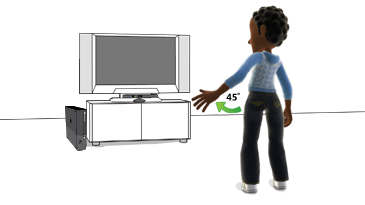
\includegraphics{figures/kinect_pose.png}
\caption{}
\label{fig:kinect-pose}
\end{figure}

\section{Leap Motion}
The gestures currently supported are:

1 to 2 fingers

Pointer � Point to anything on screen. Move your finger past the device to expand the pointer.

1 hand + 3 or more fingers (left/right/up/down)

Navigate through your slides. See config options to invert movements.

2 hands upwards

Toggle the overview mode. Do it a second time to exit the overview.

\begin{lstlisting}
// Gestures
    if( frame.gestures.length > 0 && (now - lastGesture) > config.gestureDelay ) {
      var gesture = frame.gestures[0];

      // One hand gestures
      if( frame.hands.length === 1 ) {
        // Swipe gestures. 3+ fingers.
        if( frame.fingers.length > 2 && gesture.type === 'swipe' ) {
          // Define here since some gestures will throw undefined for these.
          var x = gesture.direction[0],
              y = gesture.direction[1];

          // Left/right swipe gestures
          if( Math.abs( x ) > Math.abs( y )) {
            if( x > 0 ) {
              config.naturalSwipe ? Reveal.left() : Reveal.right();
            }
            else {
              config.naturalSwipe ? Reveal.right() : Reveal.left();
            }
          }
          // Up/down swipe gestures
          else {
            if( y > 0 ) {
              config.naturalSwipe ? Reveal.down() : Reveal.up();
            }
            else {
              config.naturalSwipe ? Reveal.up() : Reveal.down();
            }
          }

          lastGesture = now;
        }
      }
      // Two hand gestures
      else if( frame.hands.length === 2 ) {
        // Upward two hand swipe gesture
        if( gesture.direction[1] > 0 && gesture.type === 'swipe' ) {
          Reveal.toggleOverview();
        }

        lastGesture = now;
      }
    }
\end{lstlisting}

simple reflex agent based on if-then rules (condition-action rule) \cite{russell1996}
\section{Multi-modal Systems}
Bolt's pioneering work in the ``Put That There'' system \cite{Bolt80} 
demonstrated the potential for voice and gestural interaction.  In that system, 
the hand position and orientation were tracked by the Polhemus tracker, i.e.,
the hand was essentially transformed to a point on the screen. The actual hand 
posture did not matter, even if it was not in a pointing shape. The speech also 
followed a rigid and limited command-like grammar. Even though this is early 
work, it provides some insight about the advantages of multi-modal interaction. 
As Bolt summarized in the paper, using pointing gesture allows the use of 
pronouns in the speech, with the corresponding gain in naturalness and economy 
of expression \cite{Bolt80}.

Since then, several multi-modal interaction prototypes were 
developed that moved beyond Bolt's ``Put That There'' system. Cohen et al. 
\cite{Cohen97} developed the QuickSet prototype which is a collaborative, 
multi-modal system running on a hand-held PC using pen and voice as input. They 
used a novel multi-modal integration strategy that allows speech and pen gesture 
to compensate for each other, yielding a more robust system. Rauschert et al. 
\cite{Rauschert02} developed a system called Dialogue-Assisted Visual 
Environment for Geoinformation (DAVE\_G) that uses free hand gestures and speech
as input. They recognized that gestures are more useful for expressing spatial 
relations and locations. Gestures in DAVE\_G include pointing, indicating an 
area and outlining contours. Speech and gesture are fused for commands that need
spatial information provided by the gesture. 

In this thesis, we will also explore the fusion of speech and gestures. In
addition to using deictic gestures to provide spatial information as a
complement to speech as in \cite{Rauschert02}, we will explore the use of speech as a
complement to manipulative gestures based on the finding from the user study
done by Yin et al.\cite{yin10}. They observe that manipulative gestures are at times
accompanied by adjectives and adverbs that refine the actions.

control mouse

Data fusion
Result from ChaLearn \cite{escalera2013} shows that the top ranked three teams
all used late fusion of audio and skeleton data.

Many previous efforts have focused on one form of
gesture, though some efforts have attempted to handle multiple types.

\subsection{Gesture with Distinct Hand Poses}
One group of prior work focuses on classifying a set of predefined static hand
poses frame by frame. Freeman and Roth \cite{freeman95} use histogram of local
orientations, a precursor of histogram of oriented gradients (HOGs)
~\cite{dalal05}
for hand pose recognition.
Recognition is based on selecting the feature vector in the training set that is closest to the test feature vector. Suryanarayan et al. \cite{suryanarayan2010} use a volumetric shape
descriptor computed from depth data as the feature vector, and use Support
Vector Machine (SVM) for classification.

\subsection{Gesture with Distinct Paths}
The gesture production process has a direct analogy to the
speech production process \cite{Kettebekov01}, and as a result many previous
efforts have used hidden Markov models (HMMs) to recognize gestures
with distinct paths \cite{Starner95, sharma00}. More recently, discriminative models such as
conditional random fields (CRF) and its variants, such as hidden CRF
\cite{wang06} and latent dynamic CRF (LDCRF) \cite{morency07}, have also been
applied to gesture recognition with improved recognition results.
However, discriminative models may require more data to train \cite{ng02},
and may also take more time to train as the parameter space of the model is
larger.

Morency et al. \cite{morency07} use LDCRF to learn the transition parameters
between gestures. In our case, we assume the transition between gestures for
interaction is uniform: each gesture is equally likely to transit to every
other gesture.

\subsection{Different Types of Gestures}
Keskin et al. \cite{keskin12} propose a unified framework to allow concurrent
usage of hand gestures, shapes and hand skeletons. Hand gestures are modeled
with mixture of HMMs using spectral clustering. Hand shape classification and
hand skeleton estimation are based on randomized decision forests. Hand
gesture classification is active all the time. The framework estimates a set of
posteriors for the hand shape label at each frame, and continuously use these
posteriors and the velocity vector as observation to spot and classify known
gestures. They distinguish gestures with pure motion and pure hand shape by
thresholding the magnitude of the velocity vector. However, they did not mention
handling gestures with distinct hand poses but with arbitrary movement. For this
type of gestures, it will be hard to manually set a velocity threshold to
distinguish them from gestures with distinct paths.

Oka et al. \cite{Oka02} developed a system that
allows both direct manipulation and symbolic gestures, but requires the user to
indicate the gesture type by the extension of the thumb.

\subsection{Online Recognition}
Song et al. uses LDCRF with a temporal sliding window to perform
online sequence labeling and segmentation simultaneously \cite{song12}. 
Fran{\c{c}}oise et al. \cite{francoise11} use hierarchical HMMs to model musical
gestures using motion data from the Wii remote controller, and use fixed-lag
smoothing for real-time recognition and segmentation.
Our method is similar to Fran{\c{c}}oise et al.'s, but we consider different
forms of gestures in a single framework.

\subsection{Commercial Systems}
Many commercial gesture recognition systems uses if-then rules based on
heuristics. For example, the Leap Motion
plugin\footnote{\url{https://github.com/hakimel/reveal.js/blob/master/plugin/leap/leap.js}} for the Real.js HTML5 presentation
 framework uses the number of fingers
detected and the changes in the $x$ and $y$ coordinates between consecutive
frames to detect swipe and point gestures. While if-then rules could be easy to define for
a small number of simple gestures, it may be hard for more complex gestures.
For example, it may be hard to define a circle gesture using if-then rules and
the rules may conflict with each other.

The gesture interaction provided by the Kinect-based games is
one of the popular ones. Based on the observation of the interaction
available in Kinect games, it seems that the system is only looking for one
gesture (wave) or body pose (the exit
pose\footnote{\url{http://support.xbox.com/en-US/xbox-360/kinect/how-to-use-the-kinect-hub-and-guide}}) at a time, and the rest of the time, 
it is just tracking the hand and the body.

Many public datasets for evaluating gesture recognition contain only one form
of gesture \cite{Song11, Ruffieux2013, marcel99}. The Chalearn Gesture Dataset (CGD
2011) \cite{guyon13} contains nine gesture categories corresponding to various settings and application domains.
 It contains both static postures and dynamic gestures. In this dataset, a static
posture is one in which a single posture is held for a certain duration. For a
static hand posture, the hand is held at similar positions for multiple
instances of the same gesture. In this case, the static postures also have
distinct paths so they could be handled by the same method as the dynamic
gestures.
This dataset does not contain gestures with distinct hand poses but arbitrary movement
(Table~\ref{tab:taxonomy} row 2).

\chapter{Datasets}
This chapter describes the datasets used to perform the experiment evaluations
in this dissertation.

Recent advancement in sensing technology (depth sensors, the Leap Motion
sensor\footnote{\url{https://www.leapmotion.com/}}) and computer vision
(skeleton tracking \cite{shotton13}) have brought on new possibilities in interaction techniques that depart from traditional mouse
and keyboard interfaces. Even so, many gestural
interfaces still mainly make the hands function as a mouse
with a limited number of other gestures. 

Previous research on gesture
recognition usually focuses on one form of gestures, and the evaluation is also
based on offline recognition. We believe that to design a gesture
recognition system for natural human computer interaction (HCI), we need to
start from the user interaction perspective:
what are the different types of gestures people use;
when should the system respond; and how should the model be trained or defined.
These are the questions we addressed when we develop our system.

The main contributions of this work include:
\begin{itemize}
  \item We developed a unified probabilistic framework for real-time gesture
  recognition that combines two forms of gestures.
  \item We use embedded training and hidden state information to detect
  different gesture phases, allowing the system to respond more promptly.
  \item We collected a new dataset that include two forms of gestures, a
  combination currently lacking in the community. We also propose a hybrid
  evaluation metric that is more relevant to real-time interaction and different
  types of gestures.
\end{itemize}

\section{Gesture Taxonomy for Natural Interaction}\label{sec:taxonomy}
Several gesture taxonomies have been suggested in the literature. Some of them
deal with psychological aspects of gestures \cite{kendon86, mcneill82}, while
others are inspired by an HCI perspective \cite{quek94,
quek95, Pavlovic97}. The taxonomy that seems most appropriate for natural HCI
and human-centric design was developed Wobbrock et al. \cite{wobbrock09}. Their
study is based on eliciting natural behavior from non-technical users when
interacting with a computing system. Although their user study focuses on
tabletop gestures, we believe that the results can be generalized to other
interactive interfaces. 

Wobbrock et al. classify gestures in four orthogonal dimensions. As a first
step, we focus on two of them (Table~\ref{tab:taxonomy}) and incorporate them in
designing the gesture recognition system and interface. We also further generalize the
taxonomy to encompass interaction for both vertical and horizontal displays.

\subsection{Gesture Forms and Flows}
One dimension is the \textit{form} of a gesture; we distinguish two
categories in this dimension: path and pose. The first category -- path --
contains gestures characterized by distinct paths without any distinct
hand pose. For example, a ``swipe left'' gesture is characterized by a
right to left motion, while a ``circle'' gesture is characterized by a
circular motion of the hand. In doing these, users typically hold their
hands in some natural relaxed pose. The second category of gestures is
characterized by distinct hand poses without any distinct paths. This category
of gestures is usually associated with direct manipulation of some virtual
objects on the interface.
For example, a user may use a ``point'' hand pose and move around to
point at different things on a display.

\begin{table}[t]
\caption{Taxonomy of gestures for natural interaction.}
\label{tab:taxonomy}
\centering
\begin{tabular}{|c|l|l|}
\hline
\multirow{2}{*}{\textbf{\textit{Form}}} & \textit{distinct path} & with any hand
pose
\\
\cline{2-3} 
                               & \textit{distinct hand pose} & with any path \\
\hline
\multirow{2}{*}{\textbf{\textit{Flow}}} & \textit{discrete} & response occurs
\textit{after} the user acts \\
\cline{2-3}
              & \textit{continuous} & response occurs \textit{while} the user
              acts \\
\hline
\end{tabular}
\end{table}

Another dimension is the \textit{flow} of a gesture. A gesture's flow is
discrete if the gesture is performed, delimited, recognized, and responded to
as an \textit{event} \cite{wobbrock09}. One example is the ``wave'' gesture
which has a few repetitions of left and right movement; usually we want the system to
respond at the last repetition. Flow is continuous if ongoing recognition is required
and the system should respond frame by frame, as for example during a
``point'' gesture, where we want to show the cursor on the screen
continuously moving according to the hand position. 

\subsection{Temporal Modeling of Gestures}
Making gesture interaction feel natural requires a system that responds at the
correct moment. As a result, it is important to consider the temporal
characteristics of gestures. We set a foundation for doing this by taking
account of the three phases that make of a gesture:
\begin{itemize}
  \item pre-stroke,
  \item nucleus (peak \cite{mcneill82}), and
  \item post-stroke \cite{Pavlovic97}.
\end{itemize}

``Pre-strokes'' and ``post-strokes'' are movement from and to the
rest position. The ``nucleus'' of a gesture,
as Kendon \cite{kendon86} observes, has some ``definite form and enhanced dynamic
qualities''. Every gesture must have a nucleus, which is the content-carrying
part of the gesture. Based on this theory, we expect that the lack of the
nucleus phase is how unintentional movements can be distinguished from gestures. 

Even though the end of the
post-stroke phase can be more easily detected by finding the start of the
rest position, we want to do more than this to. Since nucleus is the meaningful
part of the gesture, for a discrete flow gesture, we want the system to respond immediately at the end of the nucleus
phase instead of at the end of the post-stroke phase. To make the system more responsive,
we address the more challenging problem of detecting the start and end of the nucleus phase from the pre-stroke
and post-stroke phases. This also allows the system to respond to continuous
flow gesture immediately at the start of the nucleus phase.

\section{Related Work}\label{sec:related}
Many previous efforts have focused on one form of
gesture, though some efforts have attempted to handle multiple types.

\subsection{Gesture with Distinct Hand Poses}
One group of prior work focuses on classifying a set of predefined static hand
poses frame by frame. Freeman and Roth \cite{freeman95} use histogram of local
orientations, a precursor of histogram of oriented gradients (HOGs)
~\cite{dalal05}
for hand pose recognition.
Recognition is based on selecting the feature vector in the training set that is closest to the test feature vector. Suryanarayan et al. \cite{suryanarayan2010} use a volumetric shape
descriptor computed from depth data as the feature vector, and use Support
Vector Machine (SVM) for classification.

\subsection{Gesture with Distinct Paths}
The gesture production process has a direct analogy to the
speech production process \cite{Kettebekov01}, and as a result many previous
efforts have used hidden Markov models (HMMs) to recognize gestures
with distinct paths \cite{Starner95, sharma00}. More recently, discriminative models such as
conditional random fields (CRF) and its variants, such as hidden CRF
\cite{wang06} and latent dynamic CRF (LDCRF) \cite{morency07}, have also been
applied to gesture recognition with improved recognition results.
However, discriminative models may require more data to train \cite{ng02},
and may also take more time to train as the parameter space of the model is
larger.

Morency et al. \cite{morency07} use LDCRF to learn the transition parameters
between gestures. In our case, we assume the transition between gestures for
interaction is uniform: each gesture is equally likely to transit to every
other gesture.

\subsection{Different Types of Gestures}
Keskin et al. \cite{keskin12} propose a unified framework to allow concurrent
usage of hand gestures, shapes and hand skeletons. Hand gestures are modeled
with mixture of HMMs using spectral clustering. Hand shape classification and
hand skeleton estimation are based on randomized decision forests. Hand
gesture classification is active all the time. The framework estimates a set of
posteriors for the hand shape label at each frame, and continuously use these
posteriors and the velocity vector as observation to spot and classify known
gestures. They distinguish gestures with pure motion and pure hand shape by
thresholding the magnitude of the velocity vector. However, they did not mention
handling gestures with distinct hand poses but with arbitrary movement. For this
type of gestures, it will be hard to manually set a velocity threshold to
distinguish them from gestures with distinct paths.

Oka et al. \cite{Oka02} developed a system that
allows both direct manipulation and symbolic gestures, but requires the user to
indicate the gesture type by the extension of the thumb.

\subsection{Online Recognition}
Song et al. uses LDCRF with a temporal sliding window to perform
online sequence labeling and segmentation simultaneously \cite{song12}. 
Fran{\c{c}}oise et al. \cite{francoise11} use hierarchical HMMs to model musical
gestures using motion data from the Wii remote controller, and use fixed-lag
smoothing for real-time recognition and segmentation.
Our method is similar to Fran{\c{c}}oise et al.'s, but we consider different
forms of gestures in a single framework.

\subsection{Commercial Systems}
Many commercial gesture recognition systems uses if-then rules based on
heuristics. For example, the Leap Motion
plugin\footnote{\url{https://github.com/hakimel/reveal.js/blob/master/plugin/leap/leap.js}} for the Real.js HTML5 presentation
 framework uses the number of fingers
detected and the changes in the $x$ and $y$ coordinates between consecutive
frames to detect swipe and point gestures. While if-then rules could be easy to define for
a small number of simple gestures, it may be hard for more complex gestures.
For example, it may be hard to define a circle gesture using if-then rules and
the rules may conflict with each other.

The gesture interaction provided by the Kinect-based games is
one of the popular ones. Based on the observation of the interaction
available in Kinect games, it seems that the system is only looking for one
gesture (wave) or body pose (the exit
pose\footnote{\url{http://support.xbox.com/en-US/xbox-360/kinect/how-to-use-the-kinect-hub-and-guide}}) at a time, and the rest of the time, 
it is just tracking the hand and the body.

\subsection{Datasets}
Many public datasets for evaluating gesture recognition contain only one form
of gesture \cite{Song11, Ruffieux2013, marcel99}. The Chalearn Gesture Dataset (CGD
2011) \cite{guyon13} contains nine gesture categories corresponding to various settings and application domains.
 It contains both static postures and dynamic gestures. In this dataset, a static
posture is one in which a single posture is held for a certain duration. For a
static hand posture, the hand is held at similar positions for multiple
instances of the same gesture. In this case, the static postures also have
distinct paths so they could be handled by the same method as the dynamic
gestures.
This dataset does not contain gestures with distinct hand poses but arbitrary movement
(Table~\ref{tab:taxonomy} row 2).

\section{System Overview}
We develop our system based on the understanding of the gestures for
natural interaction. Fig.~\ref{fig:system} shows an overview of our system
design.
We use a RGB-depth sensor (the Kinect sensor) for hand tracking so that we can extract
features for hand poses.

\begin{figure}[!t]
\centering
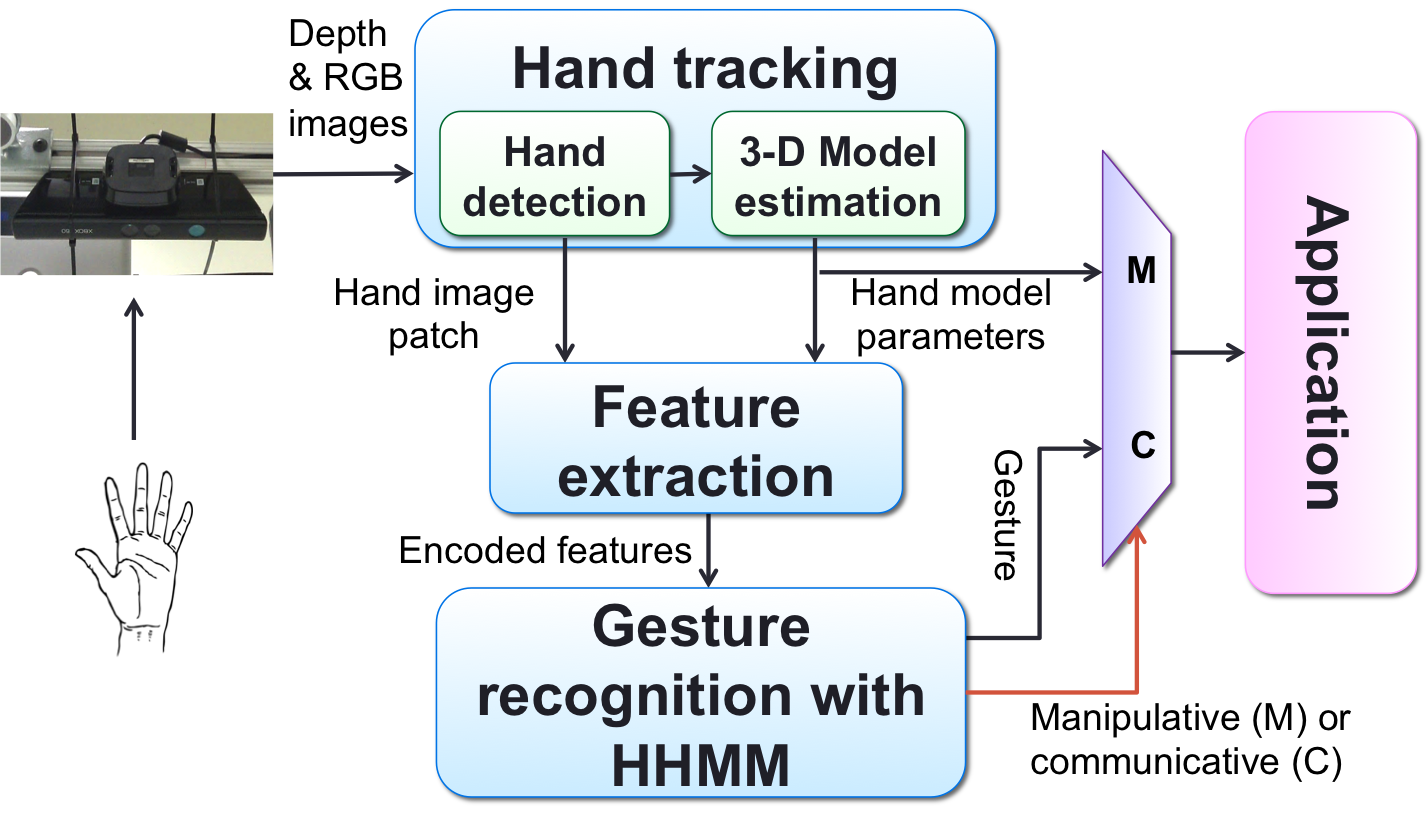
\includegraphics[width=0.8\columnwidth]{fig/system_overview.ps}
\caption{System overview.}
\label{fig:system}
\end{figure}

The gesture recognition model estimates the current most likely gesture label
and gesture phase information based on the input stream of
feature vectors. The gesture information, 
together with smoothed hand position information are sent to the application level at each time frame.

We explain the main modules in detail in the following sections.

\section{Hand Tracking and Feature Extraction}
As one category of gestures is characterized by distinct hand poses,
we need to track the full hand, rather than just treating the hand as one point. We
also need to derive a feature vector that represents the hand shape as well.

We base our hand tracking on information from the skeleton tracking of the
Kinect SDK, which is relatively robust for standing articulated body poses. At
each time frame, we use the hand joint position reported from the SDK as an
initial rough estimate of the bounding box of the hand in the depth frame.
We align the RGB and the depth frames, use skin detection to filter out
non-skin pixels in the bounding box, and then refine the bounding box using 4
interactions of CAMSHIFT \cite{bradski98}. We normalize the bounding box to a $32\times 32$ px depth
mapped image. We compute HOGs
feature from the normalized hand image (cell size =
4, number of orientation bins = 9) (see Fig.~\ref{fig:tracking}).
Since the depth data is less affected by change in illumination, we use only one
fold of normalization in the HOG feature to speed up processing.
This gives us a HOG feature of length 441 ($(32/4 - 1)\times (32/4 - 1)\times 9$). The HOG
feature has been used as a hand pose descriptor in previous work \cite{song12}
where it is often used as the input to a classifier such (e.g., Support Vector
Machine (SVM)). Our system uses principal component analysis (PCA)
to reduce the HOD dimensionality from 441 to 14, then uses it directly as part
of the input feature vector to the hidden Markov model (HMM) based recognition framework.

\begin{figure}[!t]
\centering
\includegraphics[width=0.8\columnwidth]{fig/hand_tracking.ps}
\caption{Hand tracking and hand pose feature extraction.}
\label{fig:tracking}
\end{figure}

The feature vector $\underline{x}_t$ at frame $t$ is then a concatenation of motion features and encoded HOG features. The
motion features include relative position of the hand to the shoulder joint,
velocity and and acceleration, all in 3D world coordinates. The feature vector
is computed for each input frame streamed from the sensor to form a sequence of
feature vectors.

\section{Real-Time Continuous Gesture Recognition}
The temporal model of gestures can be represented by a stochastic state machine.
Each gesture phase can in turn also be represented by a stochastic state
machine, with each state generating an observation (i.e. the feature vector).
This process can be viewed as a hierarchical HMM (HHMM) (Fig.~\ref{fig:hhmm}). If we assume
that the states in the sub-HMMs are not shared, we can collapse the hierarchical HMM
into a one-level HMM for fast inference, as the graphical model for one-level
HMM does not have loops.

\begin{figure}[!t]
\centering
\includegraphics[width=0.7\columnwidth]{fig/hhmm.ps}
\caption{State transition diagram of the hierarchical HMM representation of
gesture phases. Double-ringed states are end states.}
\label{fig:hhmm}
\end{figure}

\begin{figure}[!t]
\centering
\includegraphics[width=0.7\columnwidth]{fig/embedded.ps}
\caption{Embedding phase HMMs into an entire gesture.}
\label{fig:embed}
\end{figure}

If we have ground truth labels for the pre-stroke, the nucleus and the
post-stroke phases, we can train the sub-HMMs for each phase and each gesture
separately and then combine them \cite{yin13}. However in practice, for example
if we want users to be able to easily add their new gestures by giving a few
examples, it will be tedious to manually label the start and the end of the
three phases. In this case, we can do embedded training \cite{young1994}, i.e.
train each phase sub-HMM embedded in an entire gesture segment
(Fig.~\ref{fig:embed}).

\subsection{Unified Framework}\label{sec:unified}
We do not treat the two forms of gestures separately: gestures with
distinct paths and gestures with distinct hand poses are handled within a
single probabilistic framework. This avoids making early hard decisions (which
form of gesture it is) which will be hard to correct later. Instead, we want to
make a decision only when a response is needed, according to the flow of the
current most likely gesture, and propagate beliefs as probabilities as time progresses.

\subsubsection{Gestures with distinct paths}
We use embedded training to
combine the three gesture phases together and use normal Baum-Welch algorithm to compute the
maximum likelihood of the parameters. 

Through cross-validation, we choose to use one hidden state for pre-stroke and
post-stroke phases. We use the Bakis (left-right) model \cite{Bauer00} for the
nucleus phase, but add a backward transition from the last hidden state to the first
one for gestures with an arbitrary number of repetitions (e.g., ``wave''
gesture). We use a mixture of Gaussians to model the emission probabilities for
each hidden state. We also estimate the termination
probabilities as in \cite{yin13}.

\subsubsection{Gesture with distinct hand poses}
We use one hidden state to represent this form of gestures. Let
$s_{\text{pose}}$ be the single hidden state for the nucleus phase for a gesture
with a distinct hand pose (Fig.~\ref{fig:single}). Instead of doing embedded
training, we directly compute the maximum likelihood estimates of the mixture of
Gaussians parameters for emission probability of  $s_{\text{pose}}$. Let
$\underline{x}_1^T$ be a sequence of feature vectors corresponding to a gesture with a distinct hand pose. The feature vector sequence also contains random variations in the hand movement
path. 
We use Expectation Maximization to estimate the means, covariance matrices and
mixture probabilities for the mixture of Gaussians.

Since there is only one hidden state for $s_{\text{pose}}$, its transition
probability is 1. Its termination probability is estimated according to the
expected duration of the gesture. The self-arc on a state in an HMM defines a 
geometric distribution over waiting time \cite{murphy02}. In the case of a
single state HMM, the probability of remaining in state $s_{\text{pose}}$ for
exactly $d$ steps is $P(d) = p(1-p)^{d - 1}$, where $p = P(END|s_\text{pose})$
is the termination probability for $s_{\text{pose}}$. This means the expected
number of steps remaining in state $s_{\text{pose}}$ is $\frac{1}{p}$. We assume
that the minimum duration of a gesture with distinct hand pose is one second
(30 frames). The termination probability $P(END|s_\text{pose})$ is then set to
be less than $1/30$.

\begin{figure}[t]
\centering
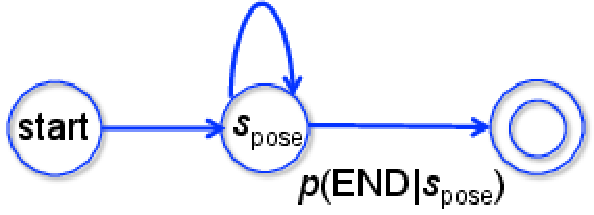
\includegraphics[width=0.5\columnwidth]{fig/single_state.ps}
\caption{State transition diagram of a single state HMM for gestures with
distinct hand poses. }
\label{fig:single}
\end{figure}

We also use one hidden state to model the rest position in a similar way.


\subsection{Real-Time Recognition}
We train the HMMs separately for each gesture, then combine them into the
hierarchical structure shown in Fig.~\ref{fig:combined}, assuming uniform
transition probabilities among gestures.
We allow sharing of the hidden states for pre-stroke and post-stroke phases for all the gestures. 

The hierarchical model allows us to do simultaneous segmentation and
recognition. We want to avoid doing segmentation first and then find the most
likely HMM for the given sequence, because segmentation based on
differentiating rest position versus non-rest position will not allow the system
to respond fast enough. We want the system to respond at the beginning of the
post-stroke phase rather then at the beginning of the rest position. In
addition, making a hard decision on segmentation can introduce errors that
are hard to correct later. 

For fast inference, we
flatten the hierarchical HMM into a regular HMM by creating an HMM state for
every leaf in the HHMM state transition diagram \cite{murphy02}. Each
hidden state $s_{GPN}$ in the flattened HMM can be indexed by three variables:
$G$ is the gesture it belongs to, $P$ is the phase it belongs to, and $N$ is its
position in the left-right model. For example, hidden state $s_{1n2}$ represents the
second hidden state in the nucleus phase of gesture 1.

\begin{figure}[t]
\centering
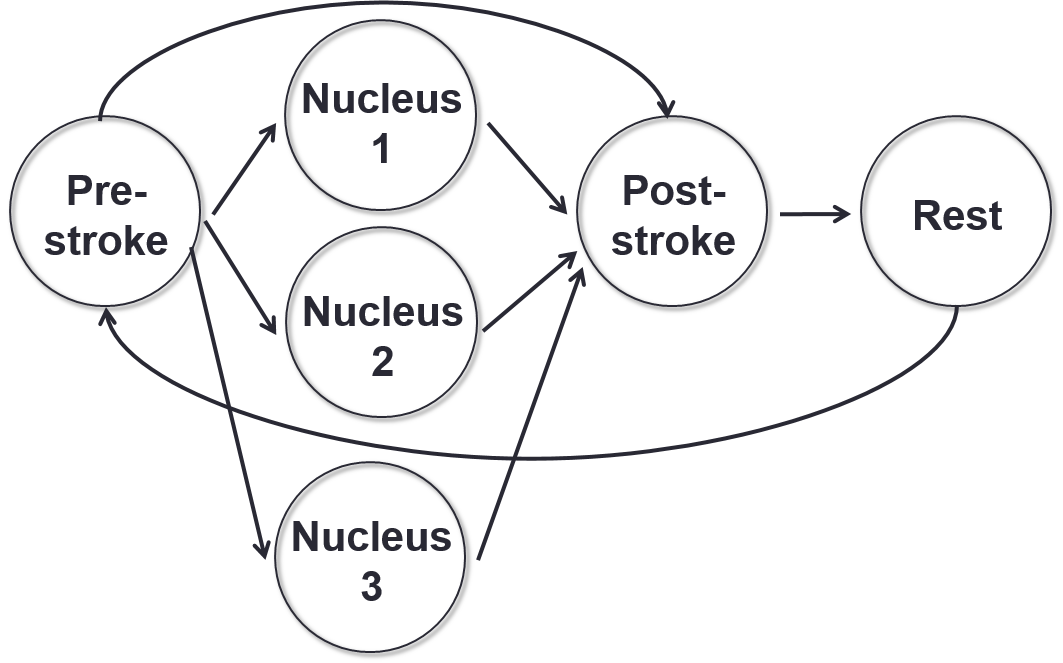
\includegraphics[width=0.7\columnwidth]{fig/combined.ps}
\caption{Hierarchical HMMs for all gestures.}
\label{fig:combined}
\end{figure}

\subsection{Online Inference}
Once we have a trained model, we use fixed-lag smoothing \cite{murphy02} to do
online inference on the flattened HMM for real-time gesture recognition.
Fixed-lag smoothing is a modified forward-backward algorithm. Unlike online
filtering, which estimates the belief state at current time $t$ using forward
pass only, we estimate the state at $t - L$, given all the evidence up to the
current time $t$, i.e., compute $\gamma_{t - L}(s) \eqdef P(S_{t -
L} = s|\underline{x}_1^t)$, where $L > 0$ is the lag. Introducing lag time is a
tradeoff between accuracy and responsiveness. Using some future evidence to
smooth the estimate can increase the accuracy while adding some delay. However
if the delay is small, it might be unnoticeable.
In the Experiment Evaluation section (Section~\ref{sec:evaluation}), we show
details about the relationship between $L$ and the recognition performance.

Fixed-lag smoothing can be implemented efficiently. We compute forward
probabilities $\alpha_t$ normally and keep a history window of $\alpha_{t -
L}\ldots\alpha_t$. At every time frame, we compute backward probabilities
$\beta$ from current time $t$ to $t - L$. Then we can compute
\begin{align}
\gamma_{t - L} = \alpha_{t - L} \cdot \beta_{t - L}
\end{align}  
The time complexity at each time frame is $O(N_s^2L)$ where $N_s$ is the total
number of hidden states in the flattened HMM. Note that at time $t$, the belief
state at $t - L$ is committed, while the belief state from $t - L + 1$ to $t$ will still be revised later.

We can then compute the most likely hidden state at $t - L$:
\begin{align}
\hat{s} = \arg\max_s \gamma_{t - L}(s)
\end{align}
We map the most likely hidden state to the gesture label it
belongs to (including the rest position) and the gesture phase. In this way
we achieve simultaneous segmentation and recognition.

Gesture events are detected at the boundary of a phase change: start pre-stroke,
start gesture nucleus and start post-stroke. This information, together with the
gesture label for the nucleus phase, are sent to the application level.

\begin{figure}[t]
\centering
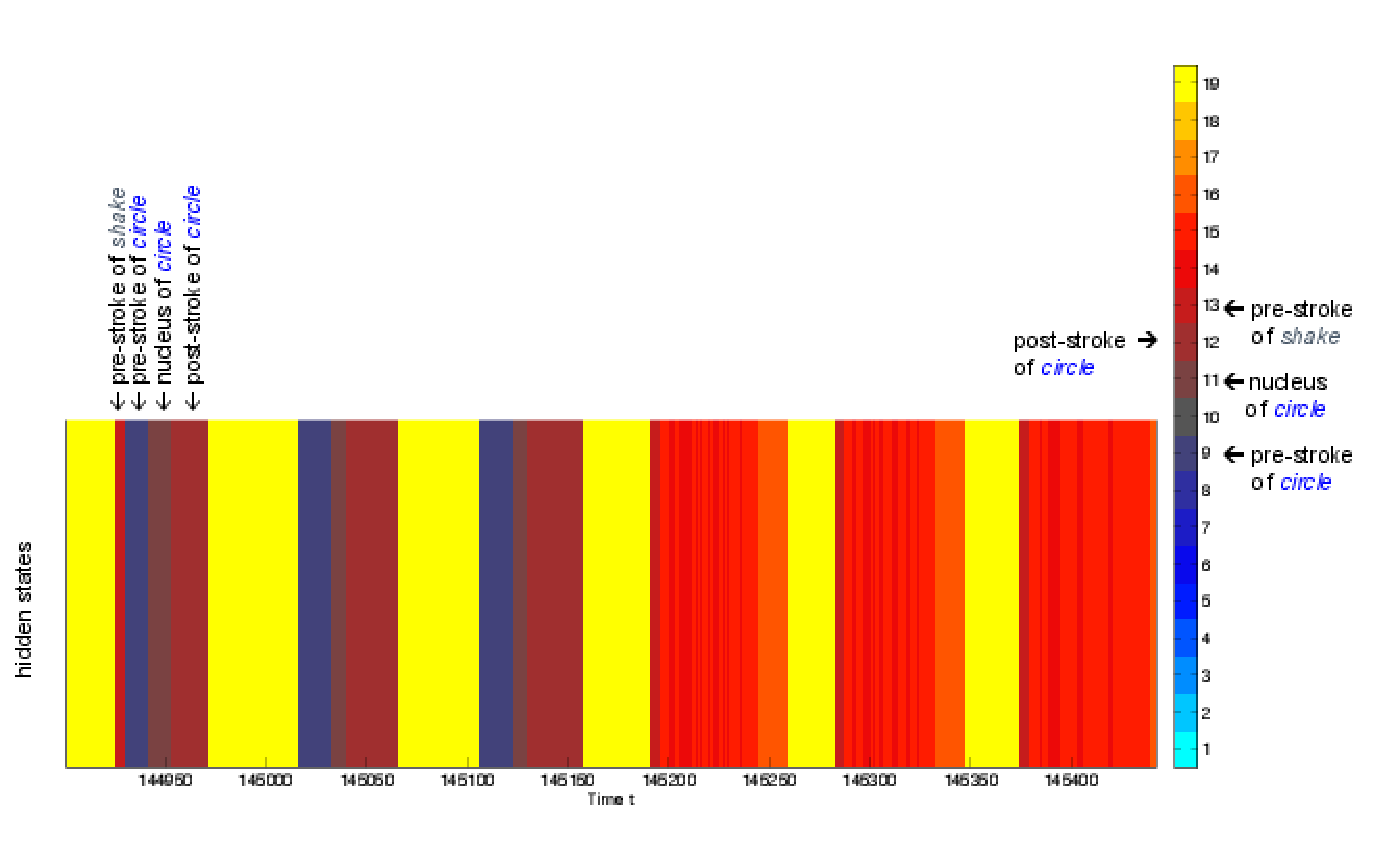
\includegraphics[trim=0 5mm 0
5mm, clip, width=1.1\columnwidth]{fig/circle_shake_label.ps}
\caption{Most likely hidden states using fixed-lag smoothing. Different colors indicate different hidden states. Yellow indicates rest position.}
\label{fig:visual_hidden}
\end{figure}

Fig.~\ref{fig:visual_hidden} shows a visualization of the
most likely hidden states based on the online fixed-lag smoothing inference
with $L = 5$.
This is based on an input sequence of 6 gestures. The first 3 gestures are
``circle'' and the last 3 gestures are ``shake hand'' gestures. Notice that in
the first segment, at the beginning, the most likely hidden state is the
pre-stroke for ``shake hand'', but since we do not need to respond at this time,
the wrong estimate does not matter. After a few more frames, the estimates are
updated to have the correct most likely gesture label and the system
responds correctly when it detects the start of the post-stroke of ``circle''
gesture.

\section{Data Collection and User Study}
Previous related work do not appear to have gesture data sets
that include both gestures with distinct paths and gestures with distinct hand
poses. To evaluate our method, we collected a dataset with a vocabulary of 7
one-hand/arm gestures focusing on combining these two forms of gestures. They
are also chosen to span over different potential difficulties (see the comments in Table~\ref{tab:gestures}).

\begin{table}
\caption{List of gestures recorded in the dataset.}
\label{tab:gestures}
\centering
\begin{tabular}{|c|l|l|l|}
\hline
\# & Name of gesture & Form & Comment \\
\hline
1 & Swipe left & distinct path & simple path \\
\hline
2 & Swipe right & distinct path & simple path \\
\hline
3 & Circle & distinct path & complex path \\
\hline
4 & Horizontal wave & distinct path & has arbitrary repetitions \\
\hline
5 & Point & distinct hand pose & arbitrary path \\
\hline
6 & Palm forward & distinct hand pose & arbitrary path \\
\hline
7 & Grab & distinct hand pose & arbitrary path \\
\hline
\end{tabular}
\end{table}

The dataset contains data from 10 participants each
doing 4 sessions. All the participants are university students.
The participants were shown video demonstration of each gesture at the beginning. 

\subsection{Recording Setup and Procedure}
In each session, the participant stands at about 1.5m from the Kinect
for Windows sensor (version one), and performs each gesture 3 times
according to the text prompts on a screen indicating the name of the gesture to
perform.
The order of the gestures is random and the time between each gesture is random
(between 2s and 6s). The first 2 sessions have ``Rest'' prompts between each
gesture, telling participants to go to the rest position (hands relaxing at the
side of the body), and the second 2 sessions do not have ``Rest'' prompts so
participants can choose to rest or not between consecutive gestures. This too
distinguishes the dataset from previous ones \cite{Ruffieux2013, guyon13} where
gestures are always delimited by rest positions.

Unlike Ruffieux et al. \cite{Ruffieux2013}, we do not show video demonstration
every time the participants perform a gesture because we want a
realistic scenario. In real practice, it is unlikely that a user will follow a
video demonstration every time he/she does a gesture. The result of this is that
there will be more variations among the gestures.

To motivate movement for gestures with distinct hand poses that
require a continuous response, the text prompt asks participants to draw
random letters in the air with the specified hand pose. 

The full corpus contains $
10P \times 4S \times 7G \times 3R = 840$ gesture occurrences
where P = participants, S = sessions, G = unique gestures, R = repetitions per
gesture. There are approximately 96 minutes of continuous recording,
recorded in the raw data from the Kinect sensor, including RGB, depth and
skeleton data. Both the RGB and depth data have a resolution of
$640\times480$px. The frame rate is 30 frame per second (FPS).

\subsection{Qualitative Observations}
We find that there is considerable variations in the way participants perform
each gesture even they were given the same demonstration video. Major variations
are observed in speed, the magnitude of motion, the paths and hand poses.

For example, some participants do swipe left and right in a rather straight
horizontal line, while others have a more curved path. Some participants start
the circle gesture at the bottom, while others start at the top. Some
participants do swipe left and right with a palm forward pose while others have
less distinct hand poses (hand is more relaxed). However, within users, they are
quite consistent within each gesture. 

\subsection{User Preferences}
We did a survey with the participants with questions that can influence
gesture interface design. We asked them, given a gesture input interface:
\begin{itemize}
  \item Whether they prefer predefined gestures or user defined gestures: 90\%
  of the participants prefer to be able to define their own gestures if necessary while 10\% of them prefer to following prefined
gestures completely. As no one prefers to define their own gestures at the very
beginning either.
\item How to define gestures: 80\% prefer defining gesture by 
performing the gestures themselves; no one prefers to
define gestures solely via rules written in terms of positions and directions
of movement of the hands.
However 20\% prefer to being able to do both.
\item Number of repetitions per gesture for training: 50\% are willing to give a
maximum of 4 - 6 examples, 40\% are willing ot give 1 - 3 examples, and 10\% are
willing to give more than 13 examples. So average maximum is about 5
repetitions.
\item Number of gestures for an application: 80\% think 6-10 gestures are
appropriate and easy to remember for a given application, 20\% prefers 1 - 5
gestures.
\item Intuitiveness of the gesture vocabulary for PowerPoint presentation:
average score is 4 out of 5 where 5 is very intuitive.
\end{itemize}

\subsection{Implications for Gesture Interaction Interface}
Based on our observation of the large variation in gesture execution among
users and small variations within users, and the fact that a majority of
participants preferring defining their own gestures if they do not the
predefined gestures, we suggest that it may be more important to optimize user
dependent recognition. As no one prefers to define their own gesture at the very
beginning, it also means that having a reasonable predefined gesture set and
basic user independent model for recognition will be useful too.

Recognition methods based on examples will allow users to train models of their
own gestures easily. We also need to develop methods that
require relatively few training examples.

\section{Hybrid Performance Metric}
Both frame \cite{song12} and event-based \cite{guyon13} metrics has been
used for evaluating gesture recognition systems. A \textit{frame} is a
fixed-length, fixed-rate unit of time. It is often the smallest unit of measure
defined by the system \cite{ward11} and in such cases approximates continuous
time.
For example, in our case, a frame is a data frame consisting of a RGB data frame, a depth data frame and a skeleton data from the
sensor at 30 FPS. An \textit{event} is a variable duration sequence of frames
within a continuous time-series.  It has a start time and a stop time.

Each of these metrics alone may not be adequate for evaluating a real-time
gesture recognition system handling different types of gestures. Frame-based
evaluation is less relevant for gestures requiring discrete responses. For the ChaLearn Gesture Challenge 2012, Guyon et al.
\cite{guyon13} use the Levenshtein distance between the ordered list of
recognized events and the ground truth events. However, such event-based metrics
that ignore timing of recognition are inappropriate for real-time
applications where responsiveness of the system matters.

Ruffieux et al. combined a time-based metric with an event-based metirc
\cite{Ruffieux2013}. Ward et al. \cite{ward11} proposed a comprehensive
scheme of combining both frame and event scoring.
We believe that all three types of information -- frames, events and
timings -- are relevant for a real-time system that responds to different types
of gestures. Hence, we developed a hybrid performance metric.

For discrete flow gestures, the system responds at the end of the nucleus phase,
so the evaluation should be event-based. Let $T_{{\text{gt\_start\_pre}}}$ be
the ground truth start time of the pre-stroke phase and
$T_{{\text{gt\_stop\_post}}}$ be the ground truth stop time of the post-stroke
phase.
A recognized event is considered a true positive (TP) if the time of response ($T_{\text{response}}$) 
occurs between $T_{{\text{gt\_start\_pre}}}$ and $T_{{\text{gt\_stop\_post}}} +
0.5\times(T_{{\text{gt\_stop\_post}}} - T_{\text{gt\_start\_pre}})$. We allow
some margin for error because there can be small ground truth timing errors.
Once a TP event is detected, the corresponding ground truth event is not
considered for further matching, so that multiple responses for the same gesture
will be penalized. We then can compute event-based precision, recall and F1 score.

For discrete flow gestures, we also define a Responsiveness Score (RS) as the
time difference in seconds between the moment when the system responds and the moment when the hand goes to a rest
position or changes gesture. Let $N_{TP}$ be the number of true positives, then
\begin{align}
RS = \frac{\sum_{i = 1}^{N_{TP}}T_{{\text{gt\_stop\_post}}} -
T_{\text{response}}}{N_{TP}}
\end{align}
A positive score means the responses are before the end of the post-strokes,
hence higher scores are better.

For continuous flow gestures, the system responds frame by frame,
so it is more appropriate to use frame-based evaluation. For all the frames that are
recognized as continuous gestures, we can compute the number of TPs by
comparing with the corresponding frame in the ground truth. Then, we can
compute frame-based precision, recall and F1 score for all the frames
corresponding to continuous flow gestures.

The average of the two F1 scores can give an overall indication of the
performance of the system.


\begin{savequote}
The retinal image produced by the hand of a gesticulating
speaker is never the same from moment to moment, yet the brain must consistently categorize
it as a hand. 
\qauthor{Semir Zeki, \textit{The visual image in mind and brain}}
\end{savequote}
\chapter{Hand Tracking}

% \section{Kinect Sensor}
% The depth sensor data from the Kinect is quite noisy. For a static scene, the
% average absolute pixel difference from the RGB camera is about 0.6\% of the maximum value (8
% bits), while the average absolute depth difference per pixel is about 4.2\%
% (347.89mm) of the maximum value (13 bits).
% 
% \begin{figure}[tbh]
% \centering
% 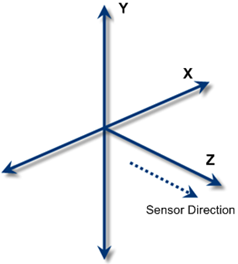
\includegraphics[width=0.3\textwidth]{figures/skeleton_space.png}
% \caption{Kinect skeleton
% space~\cite{kinect-space-14}}
% \label{}
% \end{figure}

Gesture input is particularly useful for large displays for which
keyboard and mouse input become cumbersome. There are mainly two types of
large displays: horizontal or vertical. Depending on the type of the display,
the sensor setup can be different, and hence, the characteristics of the input
data can be different. As a result, I developed different approaches for hand
tracking using data from the Kinect sensor under different system and sensor
setup.

\section{Hand Tracking for Horizontal Display}
Horizontal displays are also called tabletop displays. They are useful for
collaborative work and touch-based interaction. 

\subsection{System Setup}
Our custom tabletop structure includes four $1280\times1024$ pixel projectors 
(Dell 5100MP) that provide a $2560\times2048$ pixel resolution display. The
display is projected onto a flat white surface digitizer (GTCO Calcomp DrawingBoard V), 
which uses a stylus as an input device. The digitizer is tilted 10 degrees down 
in front, and is placed at 41in (104cm) above the floor, following FAA's design 
standard to accommodate the $5^{th}$ through $95^{th}$ percentiles of 
population. The projected displays were mechanically aligned to produce a single 
seamless large display area. The graphics card used is AMD
Radeon\texttrademark{TM} HD 6870 and the operating system used is Ubuntu 11.10.

\begin{figure}[tbh]
  \centering
  \subfigure{
	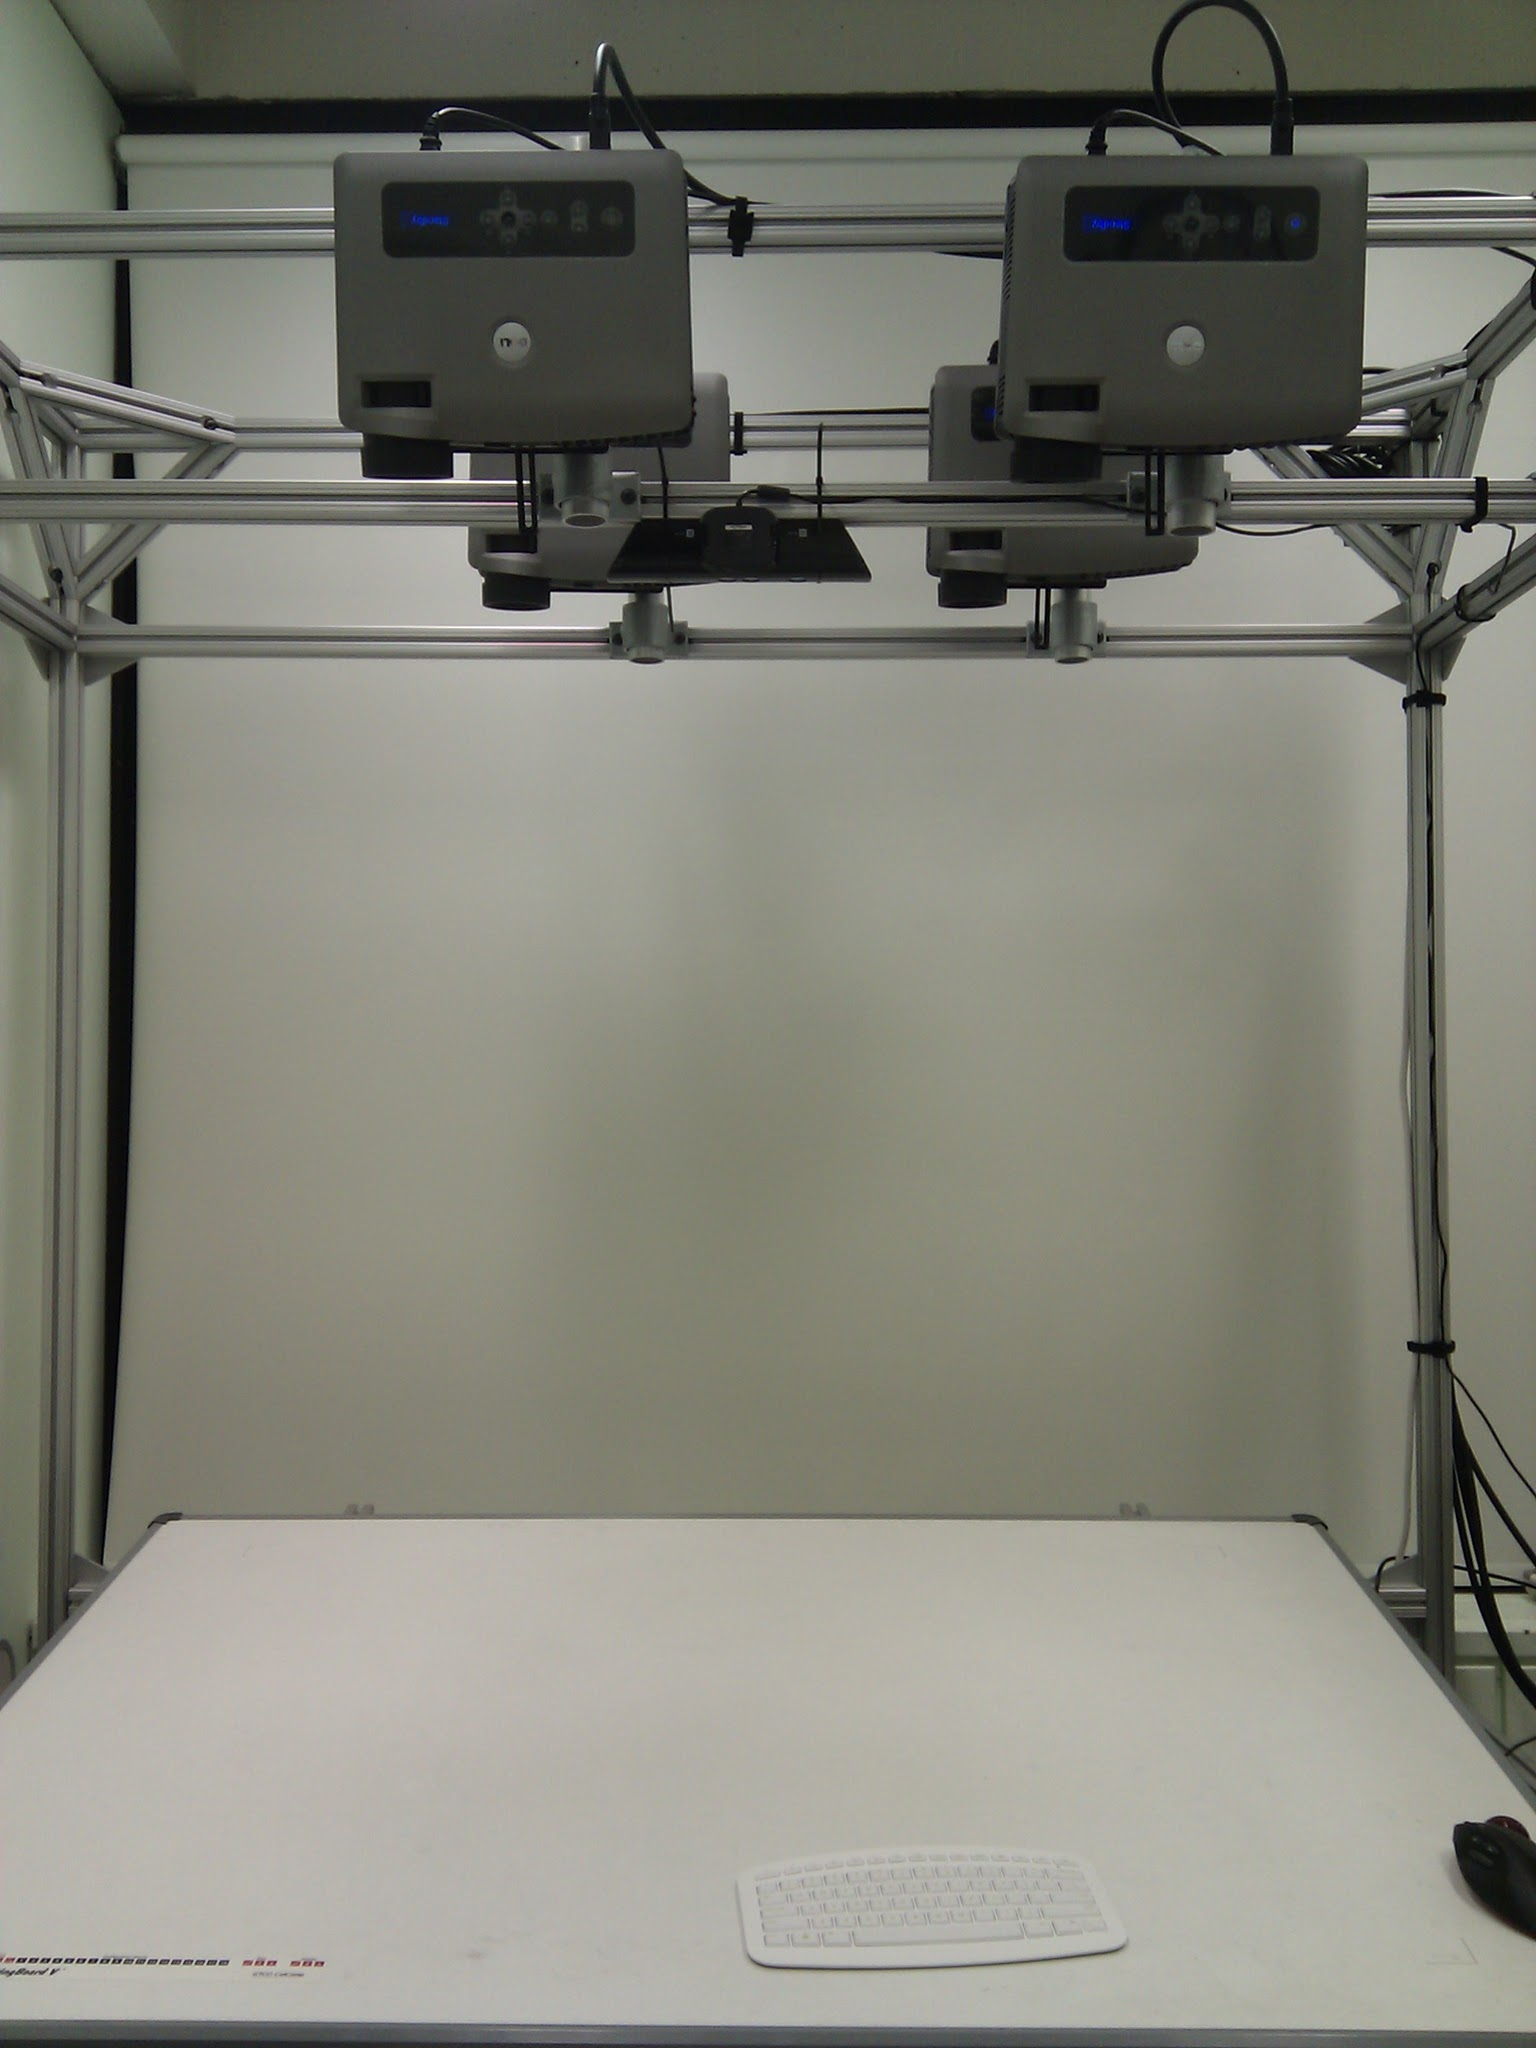
\includegraphics[width=0.4\textwidth]{figures/setup1.png} 
  }
  \subfigure{
  	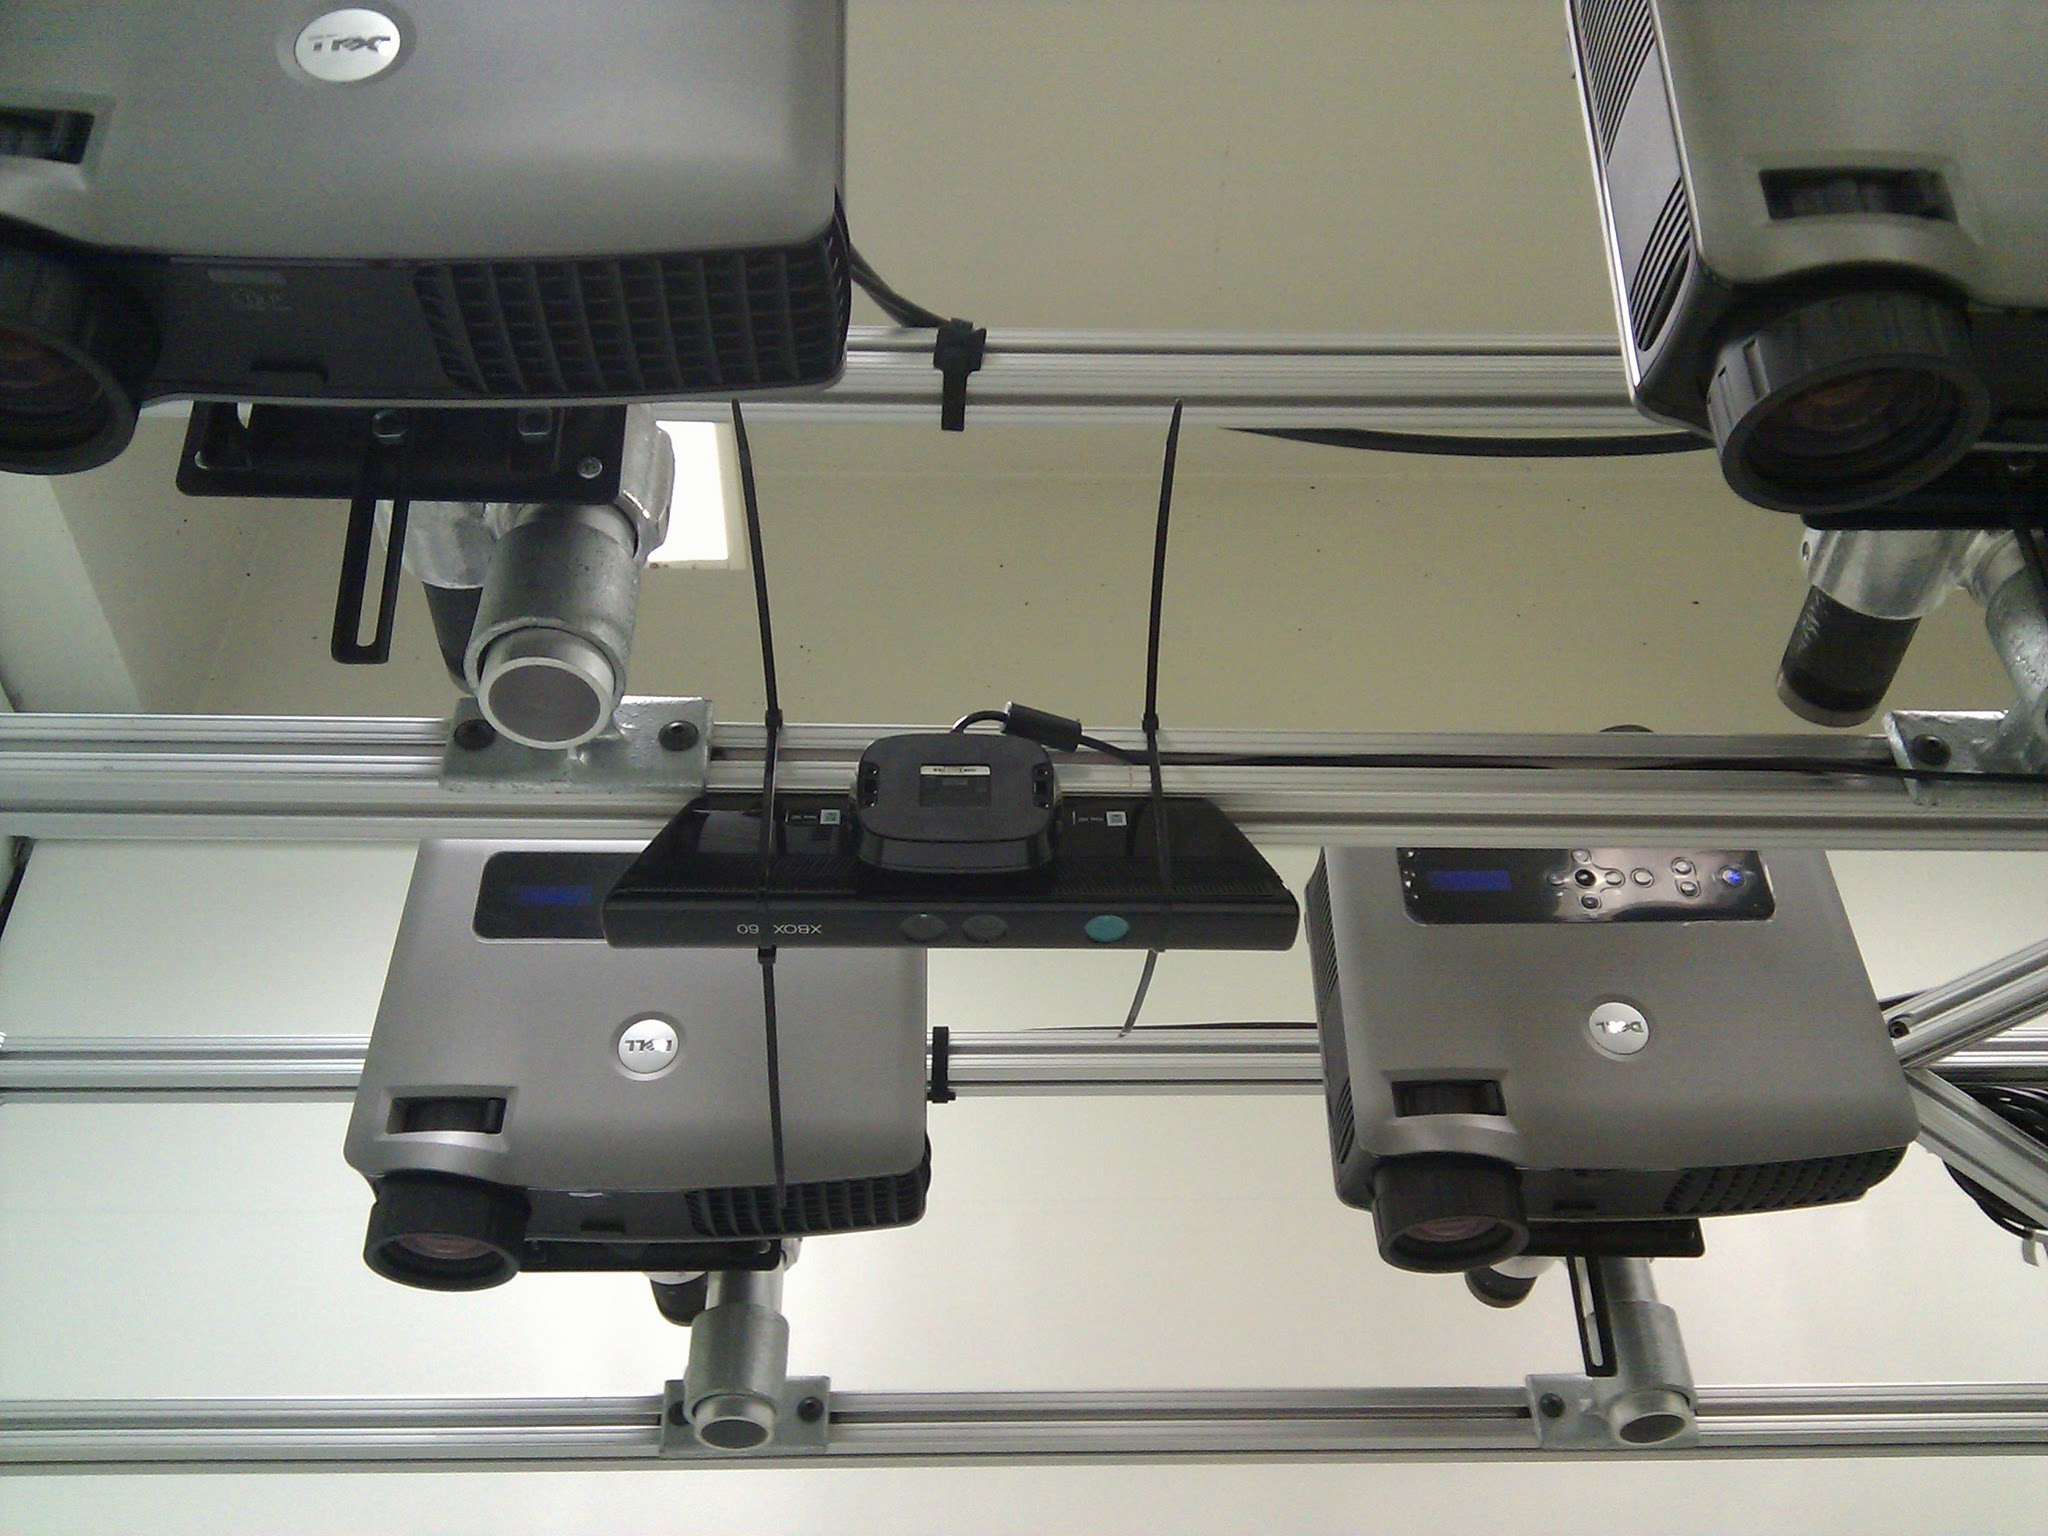
\includegraphics[width=0.4\textwidth]{figures/setup_close.png}
  }
  \caption{System setup for a horizontal display.} 
  \label{fig:setup}
\end{figure}

One Kinect sensor is placed above the center of the tabletop
at the same level of the projectors. Figure~\ref{fig:setup} shows the setup.
I use the depth data for hand tracking because it is
less sensitive to the lighting condition. This is particularly relevant for our
projection system. The Dell 5100MP projector uses a spinning color wheel to
modulate the image. This produces a visible artifact on the screen, referred to 
as the ``rainbow effect'', with colors separating out in distinct red, green, 
and blue. At any given instant in time, the image on the screen is either red, or green, or blue,
and the technology relies upon people's eyes not being able to detect the rapid 
changes from one to the other. However, when seen through a RGB camera, the
effect is very obvious, and this would greatly affect hand segmentation if I
were to use the RGB images. 

The depth sensing video
stream has a resolution of $640\times 480$ pixels with 11-bit depth value. The
depth value increases as the distance of the object from the sensor increases.
The tabletop surface is about 1.2m away from the Kinect
sensor which allows us to have a relatively good depth resolution. I use the
open source OpenNI framework\footnote{https://github.com/OpenNI/OpenNI} and its
Kinect driver\footnote{https://github.com/avin2/SensorKinect} to get both the depth and RGB data streams.

\subsection{Kinect Calibration}
In order to develop an interactive interface, it is necessary to map the point
in the depth image to the point on the display. I do this by projecting a
checkerboard image on the tabletop display, and placing some wooden blocks at
the corners of the checkerboard image to create the depth differences so that 
the depth sensor can capture these corners (see Figure~\ref{fig:calibration}).
I manually labeled 16 pairs of corresponding points on the display and the depth
image. Then I apply undistortion to the depth image and planar homography to find the mapping.

\begin{figure}[tbh]
  \centering
  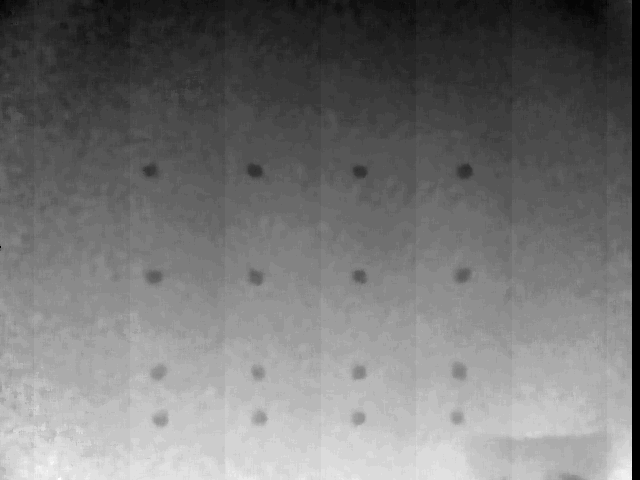
\includegraphics[width=0.5\textwidth]{figures/calibration.png} 
  \caption{Kinect calibration. The darker squares are the wooden blocks. The
  intensity of the gray level image is inversely proportional to the distance
  from the Kinect sensor.}
  \label{fig:calibration}
\end{figure}

Planar homography is a projective mapping from one plane to another. In this
case, I map points on the plane of the depth image to the points
on the plane of the display. To evaluate the result of the calibration, I
obtain a new set of manually labeled corresponding points on the display and the
depth image. I then transform the coordinates of the points on the depth image
to the coordinates on the display using the calibration result, and find the
Euclean distance (error) between the transformed coordinates and the labeled
coordinates of the points on the display. The average errors in the x-axis and
y-axis are 4.3px and 8.9px respectively, which are 0.21cm, and 0.4cm in physical distance of the
projected display. The average width of the index fingertip is about 1.4cm, so
the error is less than 30\% of the width of the fingertip. 

\subsection{Hand and Fingertip Tracking}
As the Kinect sensor is looking down at the tabletop, only the upper limbs of
the users are in the field of view of the sensor. As a result, skeleton
tracking from the Kinect SDK would not work. Hence, I developed the hand
tracking process from scratch which consists the following steps:

\begin{enumerate}
  \item Background subtraction
  \item Upper limb and hand segmentation
  \item Fingertips tracking
  \item Kalman Filtering
\end{enumerate}

The following subsections explain these steps in details.
Many of the computer vision methods I use are based on the OpenCV\footnote{http://opencv.willowgarage.com/wiki/} library and its Java interface 
JavaCV\footnote{http://code.google.com/p/javacv/}.

\subsubsection{Background Subtraction}
While the background - i.e., the tabletop - is relatively static, there is
still noise from the depth sensor. I use the averaging background method, which
learns the average and average difference of each pixel in the depth image as
the model of the background. The average values are based on the initial 30
frames with no hands in the scene; the average frame-to-frame absolute
difference is 1.3mm in our case. For the subsequent frames, any value that is
6 times larger than this (i.e., at least 7.8mm above the surface) is considered
foreground.

To clean up the background subtracted depth image, I use 1 iteration of
morphological opening to clear out small pixel noise. Morphological opening is a
combination of erosion and dilation. Both erosion and dilation are morphological
transformations. The kernel of erosion is a \textit{local minimum} operator,
while that of dilation is a \textit{local maximum} operator. Figure~\ref{fig:background} shows the difference after using morphological
opening.

\begin{figure}[h]
  \centering
  \subfigure[Without using morphological opening.] {
	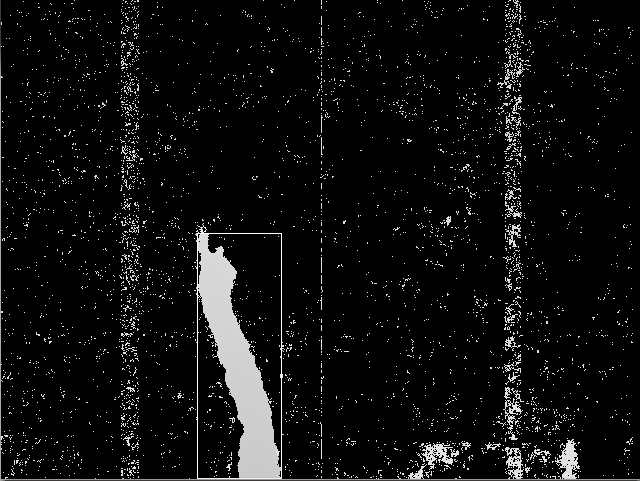
\includegraphics[width=0.4\textwidth]{figures/background_subtraction.png} 
  }
  \subfigure[Using morphological opening to clear out small pixel noise.] {
  	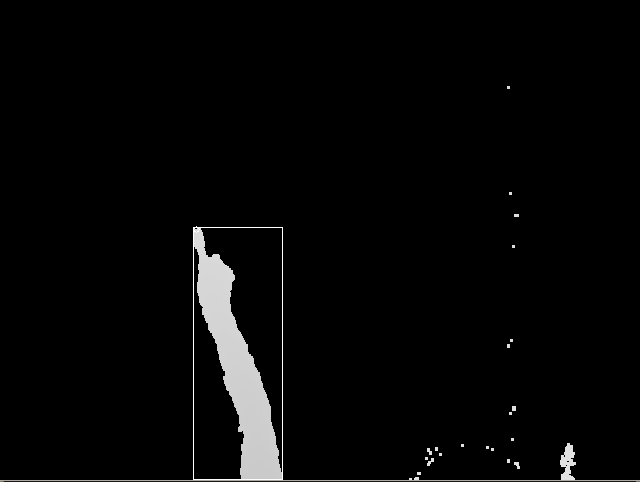
\includegraphics[width=0.4\textwidth]{figures/morphology.png}
  }
  \caption{Background subtraction.} \label{fig:background}
\end{figure}


\subsubsection{Upper Limb and Hand Segmentation}
With the cleaned up background subtracted depth image, we find connected
components by finding all contours with perimeters greater than a
threshold value of 300mm. These components are considered to be the upper limbs. 
The threshold value is roughly the lower bound of the perimeter
of a hand. We use this lower bound because the perimeter of the
upper limb changes depending on the position of the hand relative to the table.
The smallest perimeter occurs when the hand is at the edge of the table.

Each upper limb is then approximated with a convex hull and a bounding box. The
hand region is at either end of the bounding box depending on the position of 
the arm relative to the table.

\subsubsection{Fingertips Tracking}
The estimation of the hand model is based on geometric
properties of the hand. I first compute the convexity defects (shown by
the white triangular areas in Figure~\ref{fig:convexity_defects})
from the convex hull of the upper limb.
These convexity defects offer a means of characterizing the hand shape
\cite{Opencv}. As Figure \ref{fig:convexity_defects} shows, an extended finger 
has one convexity defect on each side, and the two adjacent sides of the defects
form a small acute angle (e.g., point A in Figure~\ref{fig:convexity_defects}).
We iterate through two adjacent convexity defects each time, for example, 
$\bigtriangleup B_iC_iD_i$ and $\bigtriangleup B_{i+1}C_{i+1}D_{i+1}$ in
Figure~\ref{fig:hand_defects}. If the angle between the two sides, $C_iD_i$
and $B_{i+1}D_{i+1}$ is smaller than a threshold value ($45\,^{\circ}$), we mark
the middle point of $C_iB_{i+1}$ as potential fingertips. The distance between
the \texttt{depth\_point}s (the point on the defect that is farthest from the
edge of the hull~\cite{Opencv}, e.g., $D_i, D_{i+1}$) of the adjacent convexity
defects also has to be greater than the finger width threshold value (14mm).

We further refine the fingertip position by searching in the direction of the
finger for a sharp change in the gradient of the depth value (i.e., when
the gradient is greater than 0.05). Figure~\ref{fig:five-finger} shows the
result of fingertip tracking with multiple fingers\footnote{A video of this
demo can be found at: \url{https://www.youtube.com/watch?v=_LZ4RJYBgZ4}}.

\begin{figure}[tbh]
  \centering
  \subfigure[]{
    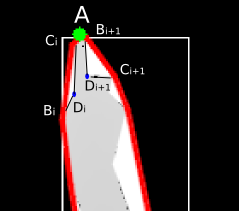
\includegraphics[width=0.23\textwidth]{figures/hand_defects.png}
    \label{fig:hand_defects}
  }
  \subfigure[]{
    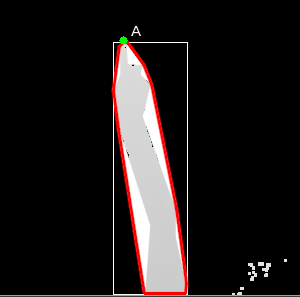
\includegraphics[width=0.23\textwidth]{figures/defects.png} 
  }
  \caption{The white triangular areas are convexity defects and the red
  outline is the convex hull.}
  \label{fig:convexity_defects}
\end{figure}

\begin{figure}[tbh]
\centering
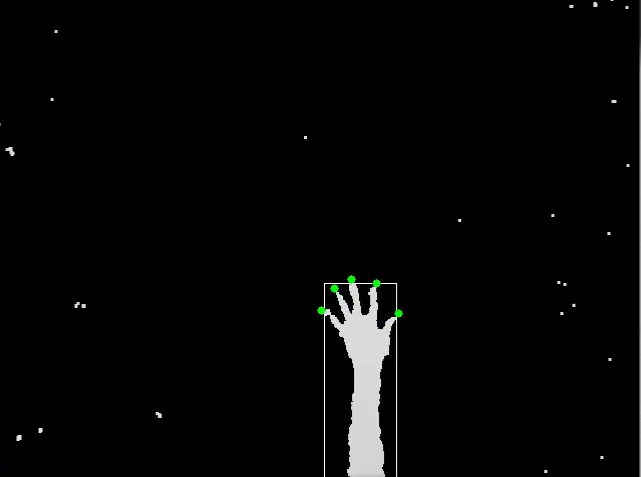
\includegraphics[width=0.7\textwidth]{figures/five_fingers.PNG}
\caption{Fingertip tracking results: green dots are detected fingertips.}
\label{fig:five-finger}
\end{figure}

\subsubsection{Kalman Filtering}
Like \cite{Oka02} and \cite{harrison11}, I use a Kalman filter to further
improve tracking accuracy. The dynamic state
of the fingertip can be summarized by a $4$-dimensional vector,
$\underline{x}_t$, of two position variables, $x$ and $y$, and two velocities,
$v_x$ and $v_y$. The measurement is a $2$-dimensional vector, $\underline{z}_t$,
of the measured $x$ and $y$ coordinates of the fingertip.

Assuming no external control, the a priori estimate $x_k^-$ of the state is
given by:
\begin{align*}
x_t^- = Fx_{t - 1} + w_t
\end{align*}
$F$ is the $4$-by-$4$ \textit{transfer matrix} characterizing the
dynamics of the system with the following values:

\begin{align*}
x_t = \begin{bmatrix}
  x   \\
  y   \\
  v_x \\
  v_y \end{bmatrix}_t, \quad
F = \begin{bmatrix}
  1 & 0 & 1 & 0 \\
  0 & 1 & 0 & 1 \\
  0 & 0 & 1 & 0 \\
  0 & 0 & 0 & 1 \end{bmatrix}
\end{align*}
assuming constant velocities, and that time is measured in frames.
$w_t$ is the \textit{process noise} associated with random events or forces
that directly affect the actual state of the system. I assume that the 
components of $w_t$ have Gaussian distribution $N(0, \Sigma_t)$ for some
$4$-by-$4$ covariance matrix $\Sigma_t$. We set the matrix $\Sigma$ with the
following values:
\begin{align*}
\Sigma = \begin{bmatrix}
  1 & 0 & 0 & 0 \\
  0 & 1 & 0 & 0 \\
  0 & 0 & 10 & 0 \\
  0 & 0 & 0 & 10 
  \end{bmatrix}
\end{align*}
The larger variance values in the last 2 values in the diagonal indicate
greater uncertainty in the velocities, as they may of course not be constant.

\subsection{3D Hand Model and Touch Detection}
I use a simplified 3D
skeletal hand model, which includes hand position, orientation and
fingertip positions, to enable touch-based direct manipulation. 

I use a line segment in 3D space to model the upper limb by computing the arm
joint position and an average of fingertip positions from the depth data. The
tabletop is modeled as a plane. In Figure~\ref{fig:point-3d}, the image on the
left shows the 3D model: the big red sphere is the arm joint and the small red
sphere is the average fingertips position. 

\begin{figure}[tbh]
\centering
\subfigure[Fingertip is not in contact with the tabletop.]{
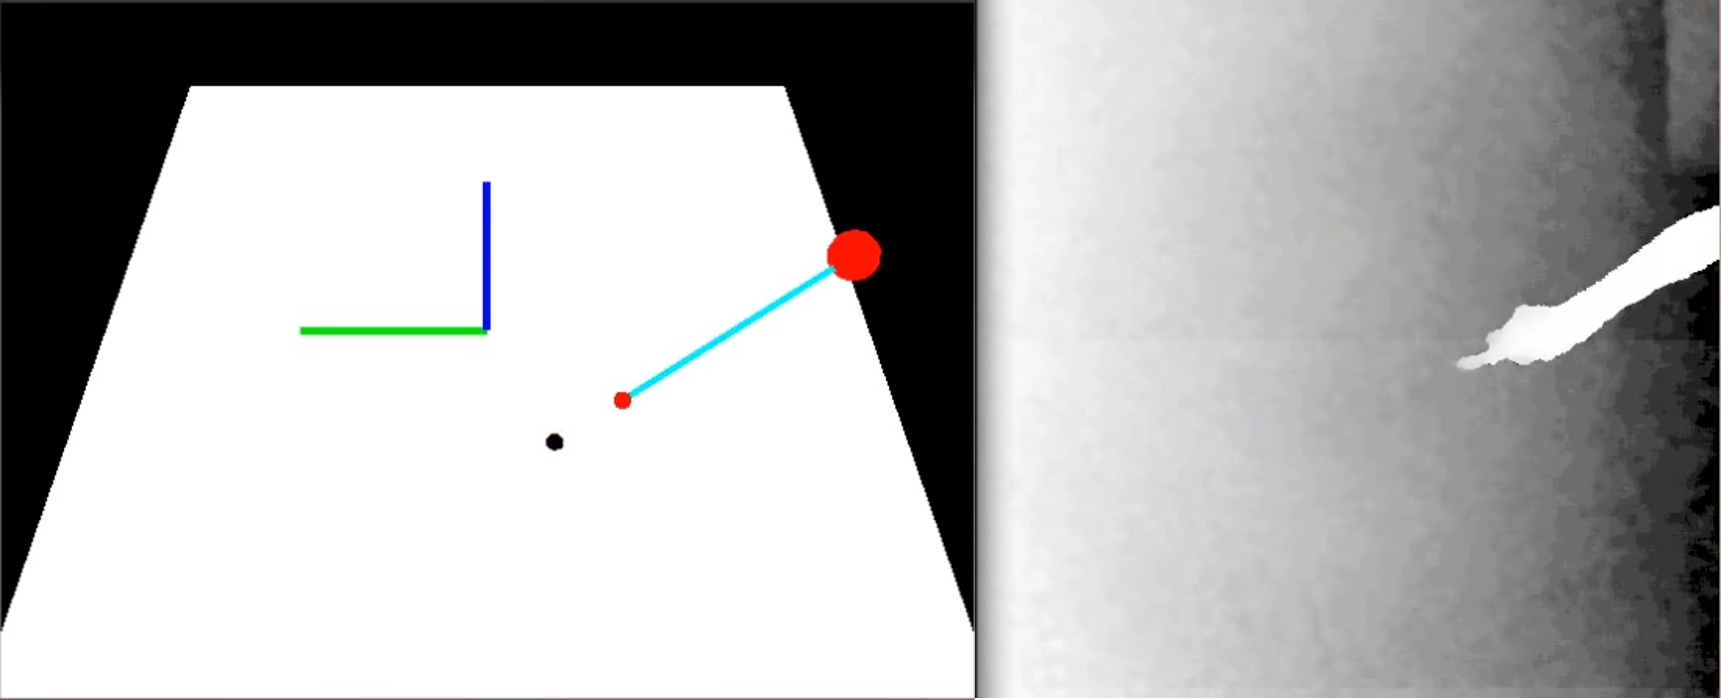
\includegraphics[width=0.7\textwidth]{figures/point_3d.png}
\label{fig:point-3d}
}
\subfigure[Finger is in contact with the tabletop.]{
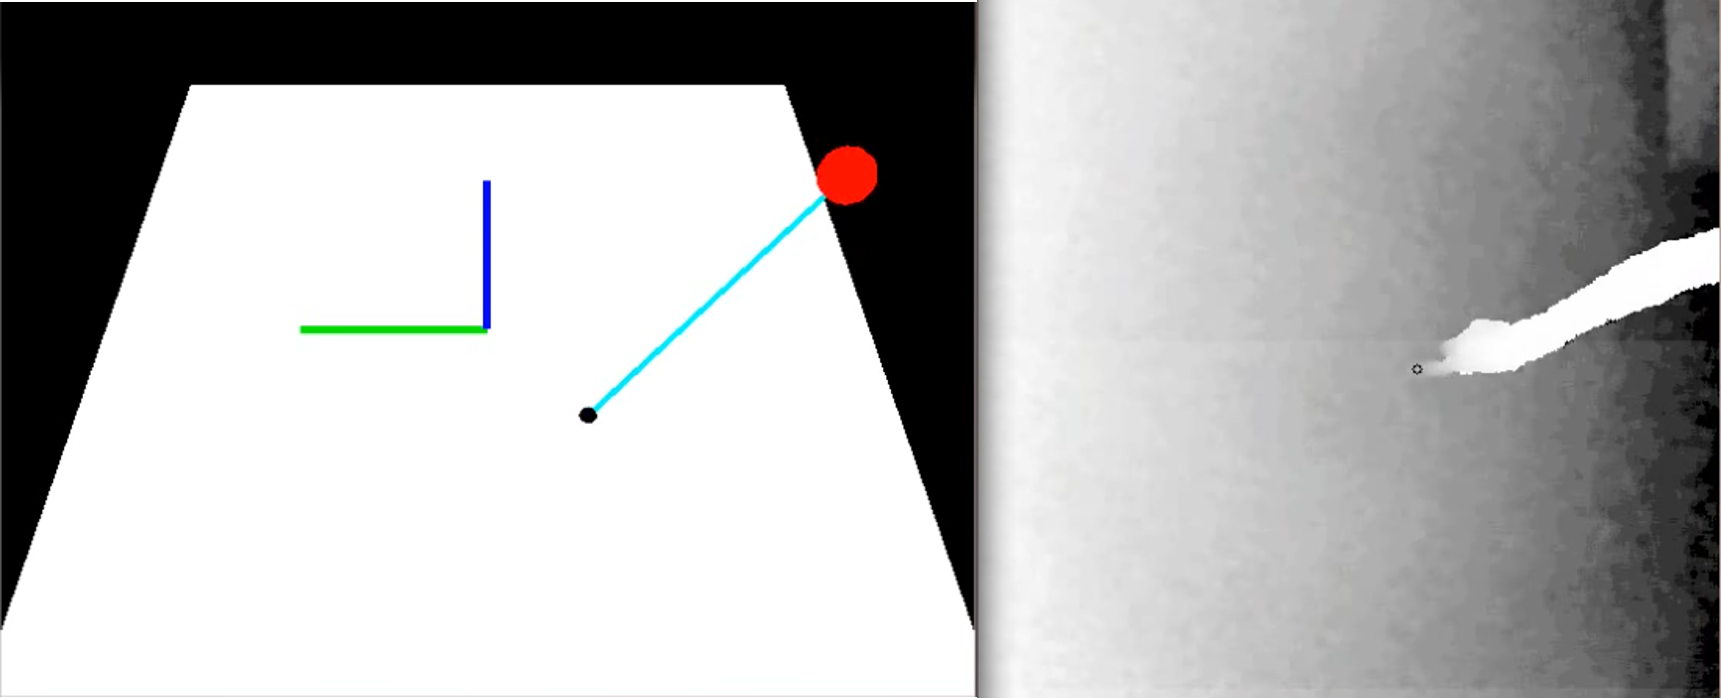
\includegraphics[width=0.7\textwidth]{figures/touch_3d.png}\label{fig:touch-3d}}
\caption{On the left are images showing 3D model of the upper limb and the
tabletop surface; on the right are are corresponding
depth mapped images. The vertical blue line is the z axis and the green
horizontal line is the y axis.}
\label{fig:3d-model}
\end{figure}

The black dot in Figure~\ref{fig:point-3d} is the intersection
between the line extended from the upper limb segment and the tabletop plane. If
the intersection is the same as the average fingertip position, the finger(s) is
in contact with the table (Figure~\ref{fig:touch-3d}). As the tabletop plane is
computed from averaged depth data, this touch detection method is more robust
than comparing the depth value of the fingertip with the depth of the tabletop
surface at one point.

\subsection{Evaluation}
Figure~\ref{fig:checkerboard} shows an example of the fingertip tracking result
on an actual display\footnote{A video of this demo can be found at:
\url{https://www.youtube.com/watch?v=8tr0ZZ-4KMc}}.
The red dot is the detected fingertip position. I evaluate the accuracy of our
fingertip tracking method by comparing the detected fingertip position with the manually labeled position in a sequence of video frames. In this evaluation, only one extended finger was used. My
method finds the fingertips with an average error (Euclidean
distance) of 5.3px, about 10mm in physical distance on the
projected display. The error rate also informs us the size of the virtual objects we should have in
our applications, i.e., they need to be at least 10mm in radius, in order to
increase the accuracy of the manipulative interaction. This result is
comparable with the accuracy in \cite{harrison11}, but my system has no
restriction on the angle of the fingers with respect to the surface.

I want to emphasize that the focus of the thesis is gesture recognition
and finding a hand model that is suitable for gestural input. As a result, I
did not push the fingertip tracking accuracy as high
as possible. I envision a better touch screen hardware will be developed
in the near future with larger size and higher resolution, and hence, touch
detection accuracy can be very high.

\begin{figure}[tbh]
\centering
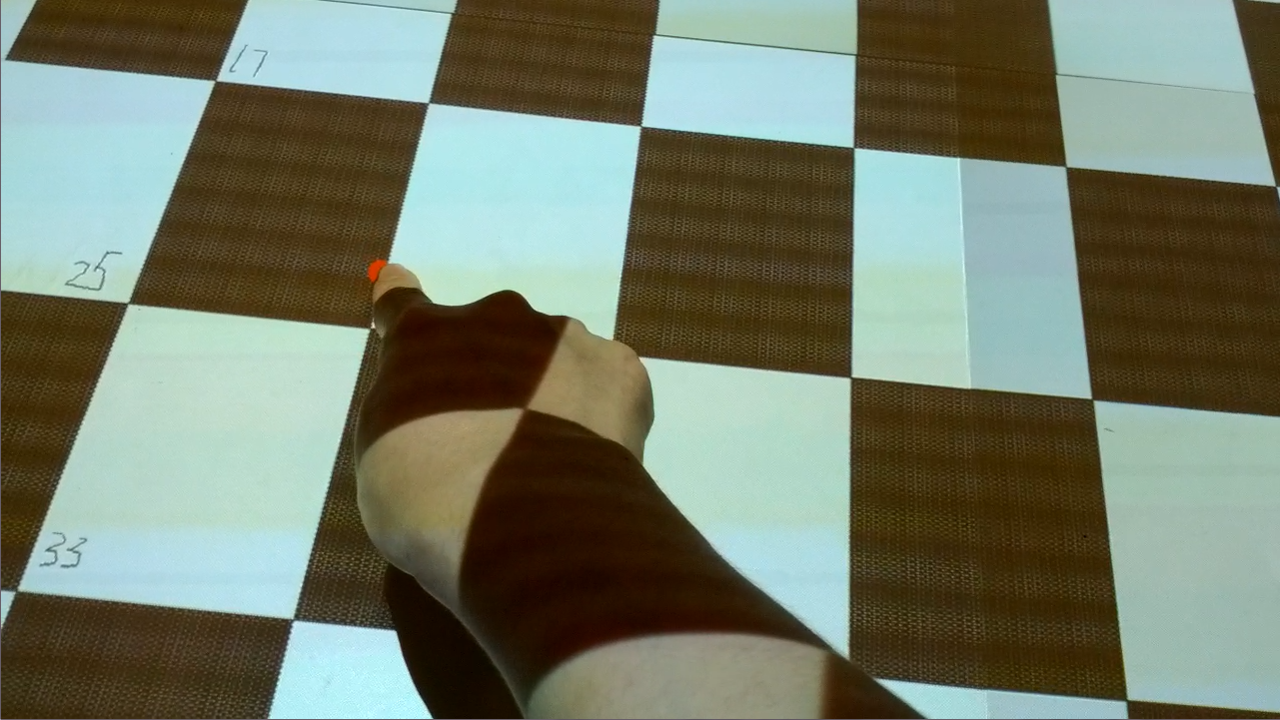
\includegraphics[width=0.9\textwidth]{figures/checkerboard.PNG}
\caption{Tracking result displayed on the tabletop surface. The red dot is the
detected fingertip position.}
\label{fig:checkerboard}
\end{figure}

\section{Hand Tracking for Seated Interaction with Vertical Display}
Currently, people mostly interact with computers while sitting in front of
desks, therefore, it is important to consider gesture input in this setting as
well. In a setup with a vertical display, the Kinect sensor is usually placed
near the display facing the user. In this case, the background scene is more
complex compared with the tabletop setup. Because of the absence of the full body and the
presence of the distracting foreground (the desk), the Kinect skeleton
tracking is less robust in the seated mode, and in particular, hand joint
tracking fails when the hands are close to the body or are moving fast.
To improve hand tracking for seated interaction, I developed a salience based
hand tracking method.

\subsection{Gesture Salience Detection}
Similar to Marcos-Ramiro et al.~\cite{marcos2013}, we define gesture
\textit{salience} as a function of both the closeness of the motion to the
observer (e.g., the camera) and the magnitude of the motion.
There are 4 steps in our method (Figure~\ref{fig:gesture-salience}).

\begin{figure*}[tbh]
\centering
\hspace{-0.6em}%
\subfigure[]{
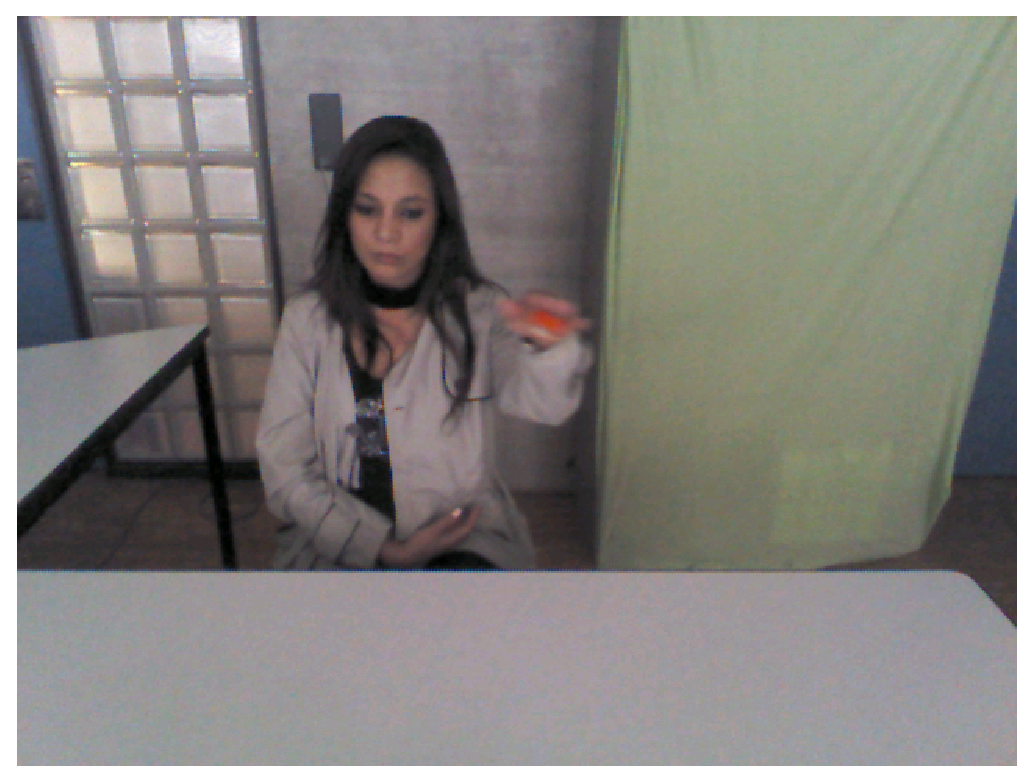
\includegraphics[width=0.19\linewidth]{figures/color.eps}\hspace{-0.6em}%
\label{fig:color}
}
\subfigure[]{
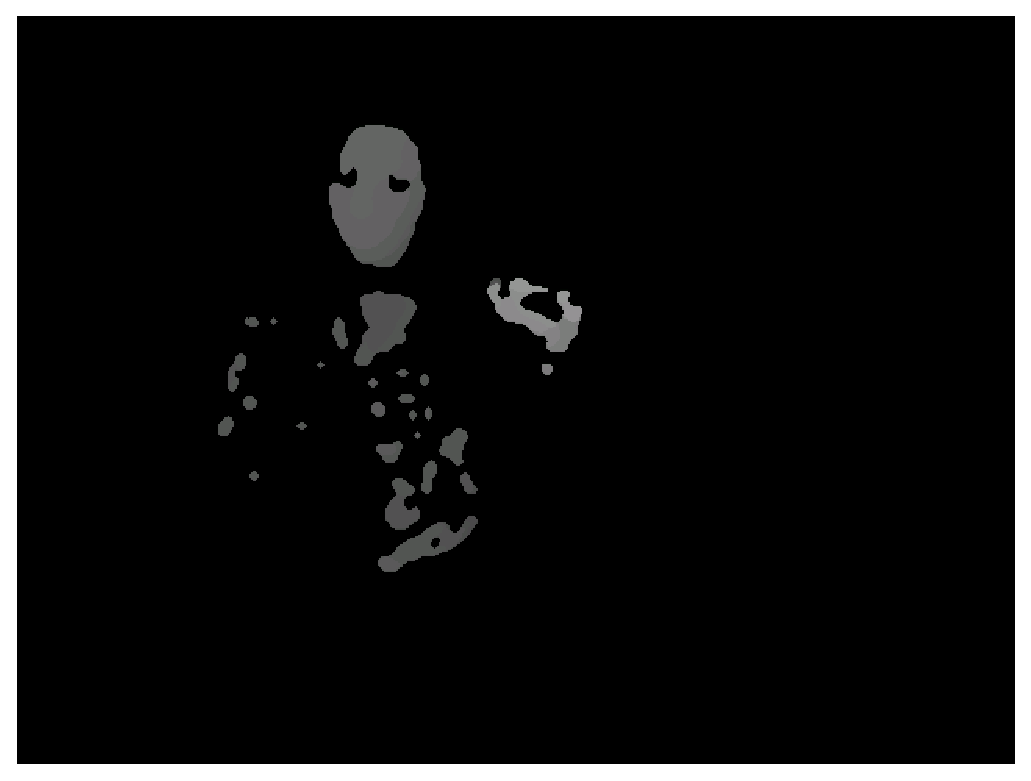
\includegraphics[width=0.19\linewidth]{figures/depth.eps}\hspace{-0.6em}
\label{fig:skin-mask}
}
\subfigure[]{
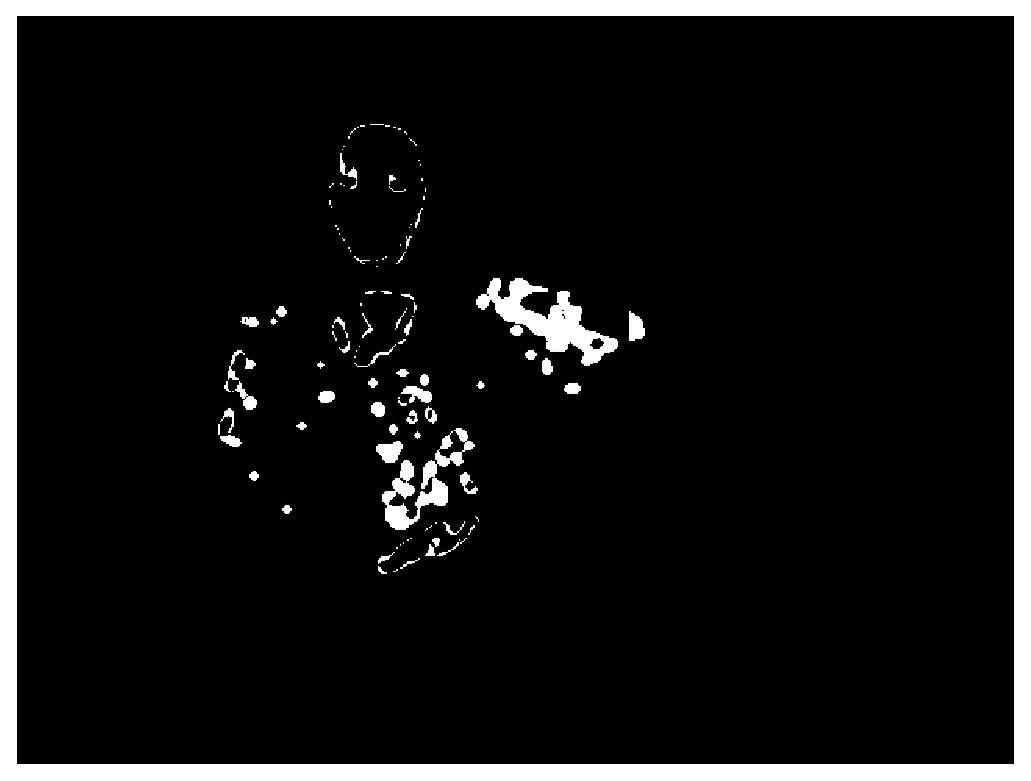
\includegraphics[width=0.19\linewidth]{figures/motion-mask1.eps}\hspace{-0.6em}
\label{fig:motion-mask}
}
\subfigure[]{
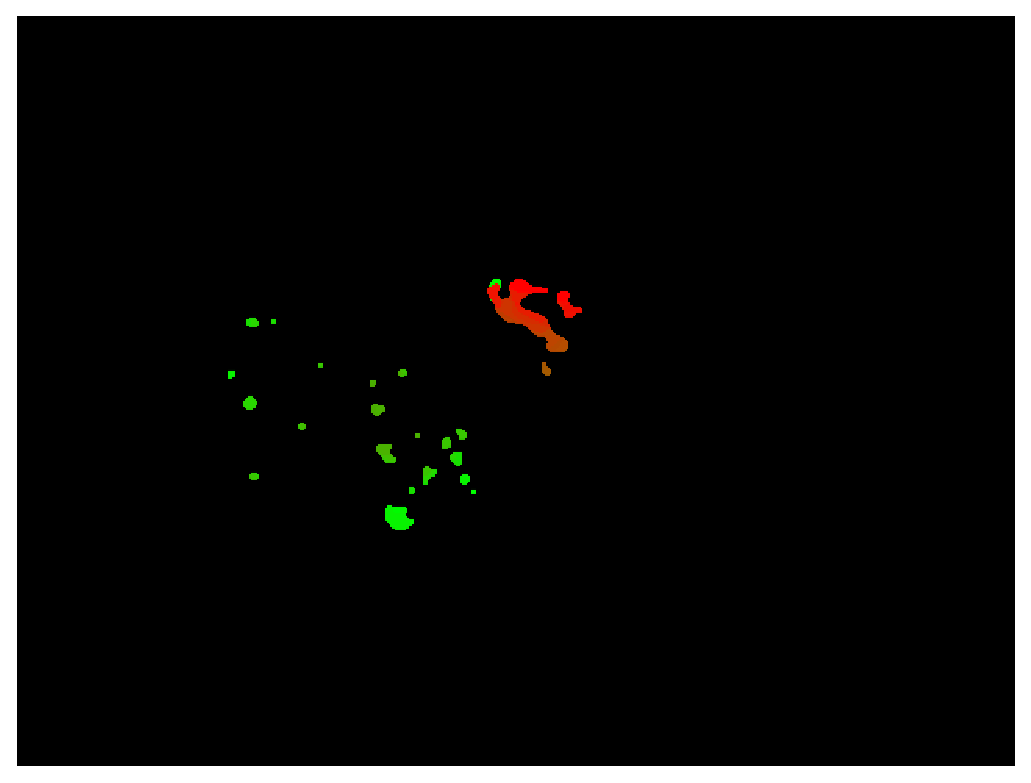
\includegraphics[width=0.19\linewidth]{figures/salient-map.eps}\hspace{-0.6em}
\label{fig:salience}
}
\subfigure[]{
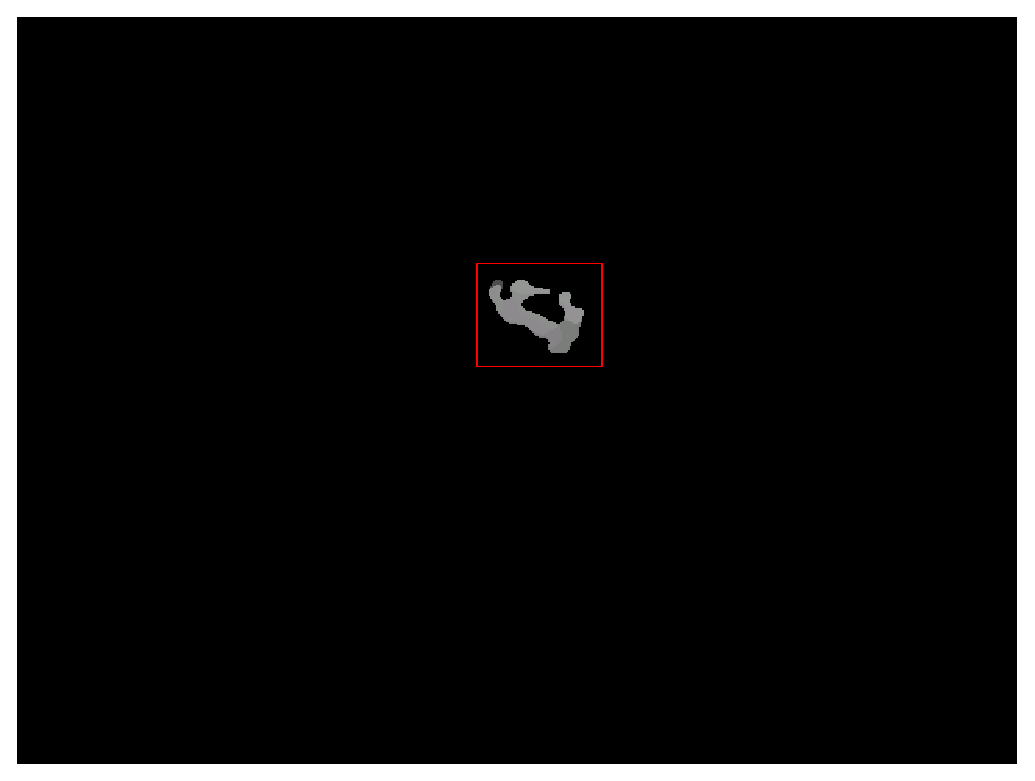
\includegraphics[width=0.19\linewidth]{figures/bounding-box.eps}
\label{fig:camshift}
}
\caption{Gesture salience detection steps: \subref{fig:color} RGB image under low lighting condition;
\subref{fig:skin-mask} depth map $D_t$ filtered by skin and user mask, $M_t^{S\wedge U}$. False detection of skin is due to
the similar colors between clothes and skin; \subref{fig:motion-mask} motion mask,  $M_{t\vee t-1}^M$, indicating moved pixels for time $t$ and $t-1$;
\subref{fig:salience} salience map with red color indicating high probability of the salience;
\subref{fig:camshift} final gesture salience bounding box, $B_t$. (Best viewed in
color. Based on data from the ChAirGest corpus.)}
\label{fig:gesture-salience}
\end{figure*}

\subsubsection{Skin Segmentation}
We use an off-the-shelf simple skin color detection method to compute a binary skin mask at
time $t$, $M_t^S$, based on the RGB image converted to YCrCb color space. We
also find the user mask, $M_t^U$ obtained from the Kinect SDK based on the depth image.
We align the two to find their intersection $M_t^{S\wedge U}$, which indicates the user's skin region.

\subsubsection{Motion Detection}
The depth data is first clipped to a maximum value $\text{depth}_\text{max}$ of
2m and then scaled to a value between 0 and 255 (1 byte):

\begin{align*}
\text{scaled} = (\text{depth}_\text{max} -
\text{depth}_\text{clipped}) \times 255 / \text{depth}_\text{max}
\end{align*}

The scaled value is inversely proportional to the depth value.
We compute the motion mask for the current depth frame based on 3 frames. We first filter each
depth frame by the user and skin mask $M_t^{S\wedge U}$, and then
smooth it through a median filter to obtain $D_t$ (Figure~\ref{fig:skin-mask}).
Equation~(\ref{eq:motion-mask}) computes the binary mask, $M_{t\vee t-1}^M$,
indicating pixels whose depth values have changed from time $t-1$ to $t$ (Figure~\ref{fig:motion-mask}).
$D_{t\vee t-1}$ is the absolute difference between $D_t$ and $D_{t-1}$, and $T$ is the threshold operator that filters out small changes in depth value
(with a threshold of 15mm).
To obtain the motion mask, $M_{t}^M$ for time $t$ only, we use $M_{t-1\vee t-2}^M$, the motion mask for $t-1$ and $t-2$ as well (see Equation~(\ref{eq:motion-mask-t}),
 AND and XOR are indicated by $\wedge$ and $\oplus$).
\begin{align}
M_{t\vee t-1}^M &= T(D_{t\vee t-1}) \label{eq:motion-mask} \\
M_{t}^M &= M_{t\vee t-1}^M \oplus (M_{t\vee t-1}^M \wedge M_{t-1\vee t-2}^M) \label{eq:motion-mask-t}
\end{align}

\subsubsection{Salience Map}
We compute histograms of depth values in both $D_t$ and $D_{t\vee t-1}$ and then apply histogram normalization to obtain cumulative distributions $H_t$ and $H_{t\vee t-1}$.
$H_t$ represents the probability of salience given a depth value, while $H_{t\vee t-1}$ represents the probability of salience given
a depth difference value. The lower the depth value or the higher the depth difference value, the higher the salience probability. We use
histogram equalization to reduce the effect of outliers, so that a single large depth value will not suppress the salience probabilities of other depth values.
The salience map (Figure~\ref{fig:salience}) can then be computed for each pixel $(x, y)$:
\begin{align*}
S_t(x, y) = H_t(D_t(x, y)) \times H_{t\vee t-1}(D_{t\vee t-1}(x, y)) \times M_t^M
\end{align*}
The multiplication of the binary motion mask $M_t^M$ allows us to consider only the motion due to the user at $t$.

\subsubsection{Salience Location}
The final step of locating the most salient region in a frame is finding the
contour, $C_t$, from the salience map $S_t$ that has a perimeter greater than
the smallest possible hand perimeter and with the highest average salience for all the pixels inside the contour.

When motion is slow, the motion mask usually indicates the edge of the moving
object. As a result, the center of $C_t$ may not be the center of the moving
object (in this case, the user's hand). Hence, we use 2 iterations of
Camshift~\cite{bradski98} on the depth image $D_t$ with a starting search location at the center of $C_t$ to refine
the final bounding box, $B_t$, of gesture salience (Figure~\ref{fig:camshift}).

\subsection{Evaluation}
Figure~\ref{fig:compare-skeleton} shows examples of our hand tracking result (red regions).
It is more reliable than the hand joint locations from the Kinect SDK. Using the
ChAirGest dataset and the same recognition method, Table~\ref{tab:comp-tracking}
compares the results using different methods to find hand positions. the same
motion features from the IMU attached to the hand are used in both cases. It
shows that using my salience detection method to extract hand position features gives 3.7\% absolute increase in gesture recognition $F_1$ score compared to using the hand joint position from the Kinect SDK.

\begin{figure*}
\centering
\subfigure[]{
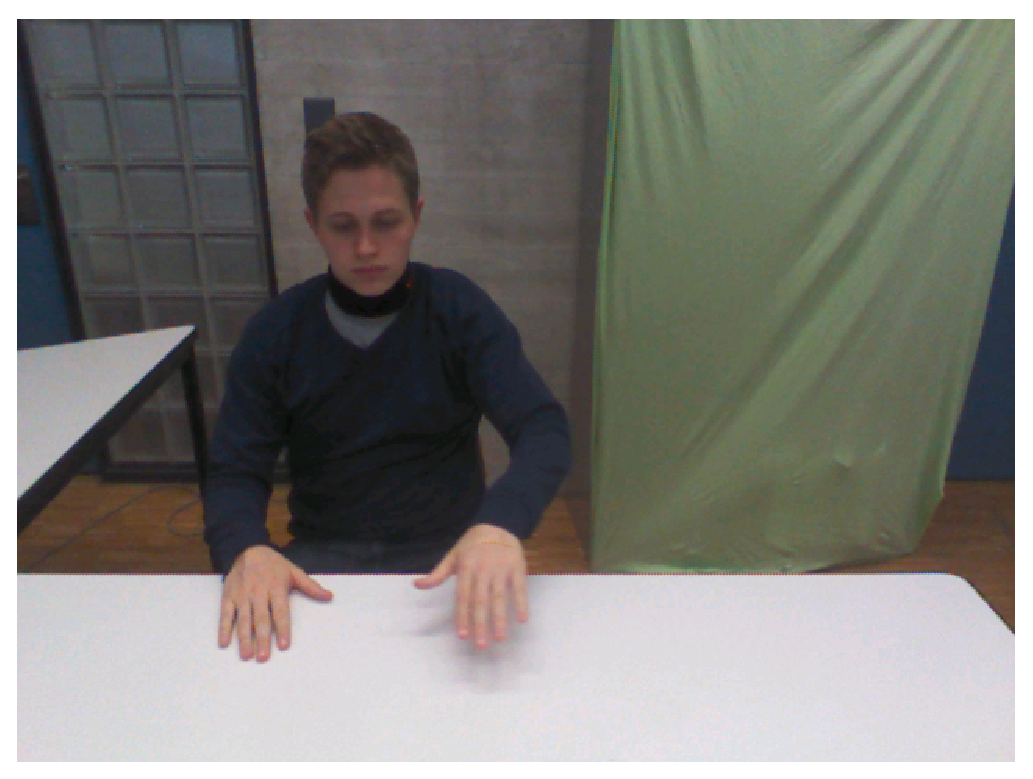
\includegraphics[width=0.23\linewidth]{figures/rotate-color.eps} \hspace{-0.6em}
}
\subfigure[]{
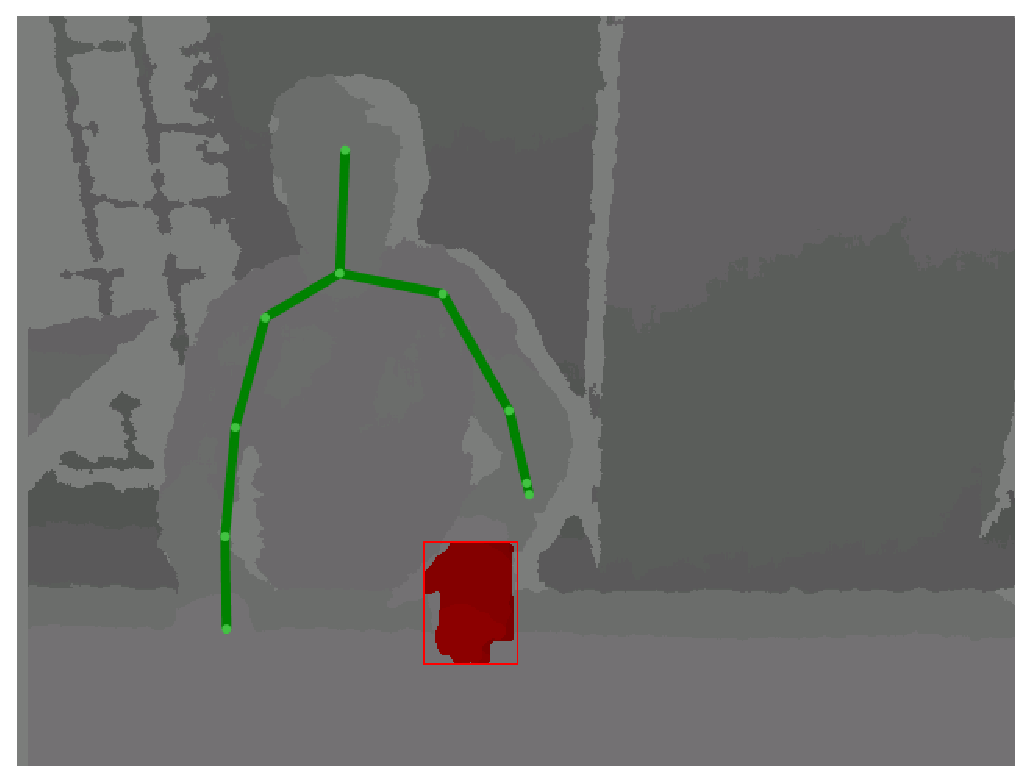
\includegraphics[width=0.23\linewidth]{figures/rotate-depth.eps} \hspace{-0.6em}
}
\subfigure[]{
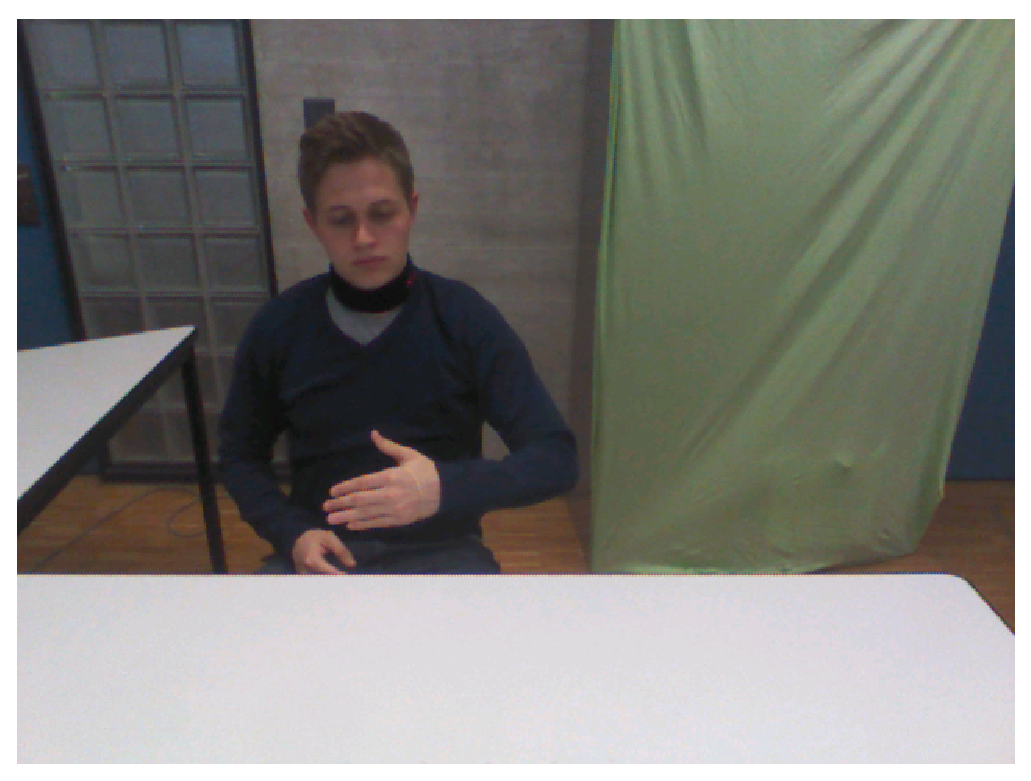
\includegraphics[width=0.23\linewidth]{figures/near-body-color.eps}
\hspace{-0.6em} }
\subfigure[]{
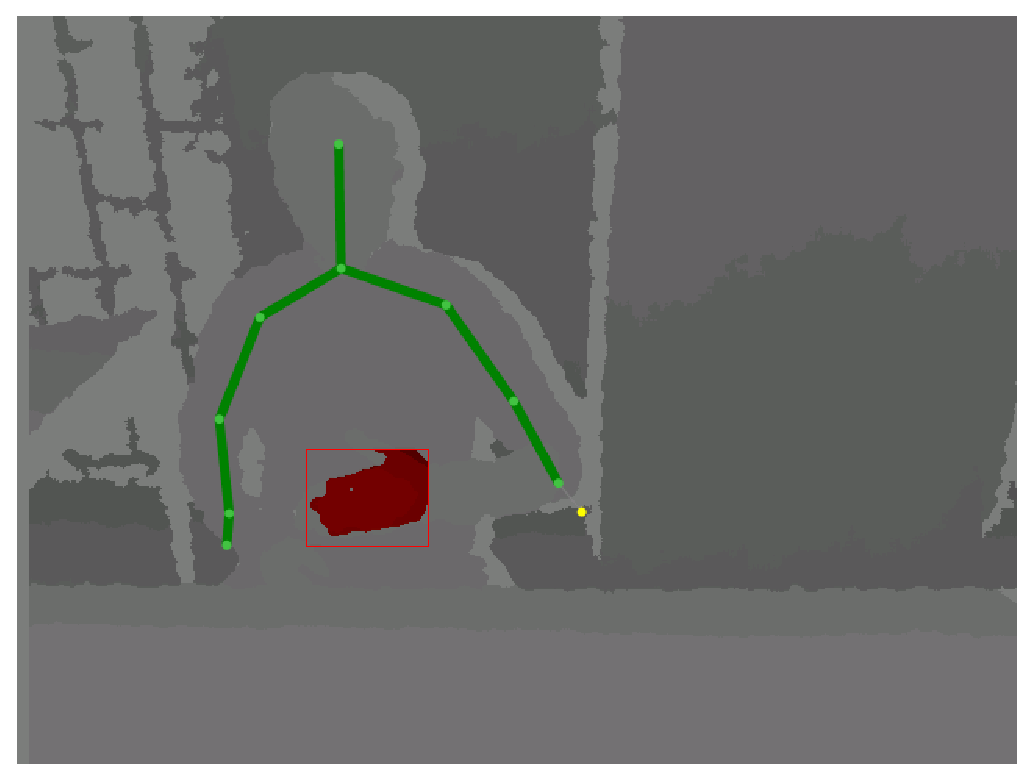
\includegraphics[width=0.23\linewidth]{figures/near-body-depth.eps}
\hspace{-0.6em} }
\caption{Comparison of hand tracking results. Our method (red region) gives more
reliable result on hand tracking compared to the off-the-shelf Kinect software
(green line). (Best viewed in color. Based on data from ChAirGest
corpus.)}
\label{fig:compare-skeleton}
\end{figure*}

\begin{table}[h]
\begin{center}
\begin{tabular}{|l|p{5cm}|p{5cm}|}
\hline
 & Hand position from salience detection & Hand position
 from Kinect skeleton \\
\hline
$F_1$ Score & \textbf{0.907 (0.01)} & 0.870 (0.02) \\
\hline
\end{tabular}
\caption{Comparison of the average 3-fold cross validation results for different
hand tracking methods using the ChAirGest dataset. Values in parentheses are
standard deviations.}
\label{tab:comp-tracking}
\end{center}
\end{table}

% \section{Hand Tracking and Feature Extraction}
% As one category of gestures is characterized by distinct hand poses,
% we need to track the full hand, rather than just treating the hand as one point. We
% also need to derive a feature vector that represents the hand shape as well.
% 
% We base our hand tracking on information from the skeleton tracking of the
% Kinect SDK, which is relatively robust for standing articulated body poses. At
% each time frame, we use the hand joint position reported from the SDK as an
% initial rough estimate of the bounding box of the hand in the depth frame.
% We align the RGB and the depth frames, use skin detection to filter out
% non-skin pixels in the bounding box, and then refine the bounding box using 4
% interactions of CAMSHIFT \cite{bradski98}. We normalize the bounding box to a $32\times 32$ px depth
% mapped image. We compute HOGs
% feature from the normalized hand image (cell size =
% 4, number of orientation bins = 9) (see Fig.~\ref{fig:tracking}).
% Since the depth data is less affected by change in illumination, we use only one
% fold of normalization in the HOG feature to speed up processing.
% This gives us a HOG feature of length 441 ($(32/4 - 1)\times (32/4 - 1)\times 9$). The HOG
% feature has been used as a hand pose descriptor in previous work \cite{song12}
% where it is often used as the input to a classifier such (e.g., Support Vector
% Machine (SVM)). Our system uses principal component analysis (PCA)
% to reduce the HOD dimensionality from 441 to 14, then uses it directly as part
% of the input feature vector to the hidden Markov model (HMM) based recognition framework.
\begin{savequote}
It is precisely this variation -- and the apparent success of our visual system
and brain in achieving recognition in the face of it -- that makes the problem
of pattern recognition so interesting.
\qauthor{Irving Biederman, \textit{Higher-level vision}}
\end{savequote}
\chapter{Hand Features and Representations}\label{chap:feature}
This chapter discusses different 
hand feature representations and encoding methods to produce feature
vectors as input to the recognition module.  One feature vector is computed
for each input frame streamed from the sensor(s) to form a sequence of feature
vectors.

As features can have different numeric ranges, to avoid features with greater
numeric ranges dominating those with smaller numeric ranges, it is important to
scale the feature vectors before feeding them  into the recognition
module~\cite{hsu10}. Hence, after computing the feature vectors, the last step
is always standardizing all the features to have 0 mean and 1 standard deviation
using all the training data. During testing, the data are standardized using the means and the standard deviations from training.

\section{Hand Motion Features}
Motion features are important for path gesture representation. 

It is relatively easy to obtain motion features from IMUs if they are present.
From the ChAirGest dataset, I use linear acceleration $(x, y, z)$,
angular velocity $(x, y, z)$ and Euler orientation (yaw, pitch, roll) from the
IMU on the hand to form a 9-dimensional feature vector
$\underline{x}_t^{\text{imu}}$ at every time frame $t$.

One limitation of IMUs is that they cannot provide hand position information. To
complement this, we can use hand position information from hand tracking in the
previous section. With the Kinect sensor data from the ChAirGest dataset and
using the gesture salience based hand tracking method, I extract the position of a gesturing hand in $(x, y, z)$ coordinates relative to the shoulder center joint to form a 3-dimensional vector $\underline{x}^\text{kinect}_t$ (should center joint position from the Kinect
SDK is relatively accurate under most situations).
Combining the two, we
have a 12-dimensional feature vector $\underline{x}_t =
[\underline{x}^\text{kinect}_t, \underline{x}^\text{imu}_t]$.
The evaluation in Table~\ref{tab:comp-motion-feature} shows that adding
position information can improve recognition accuracy further for path gestures.
Figure~\ref{fig:confusion} shows the confusion matrix based on result using
features computed from both the Kinect and the IMU sensors.

\begin{table}[tbh]
\begin{center}
\begin{tabular}{|l|p{6cm}|p{4cm}|}
\hline
 & Hand position from salience detection \& IMU,
 $[\underline{x}^\text{kinect}_t, \underline{x}^\text{imu}_t]$ & IMU only, $\underline{x}^\text{imu}_t$ \\
\hline
F1 Score & \textbf{0.907 (0.01)} & 0.890 (0.02) \\
\hline
ATSR Score & \textbf{0.923 (0.02)}  & 0.920 (0.01) \\
\hline
Final Score & \textbf{0.912 (0.01)}  & 0.895 (0.01) \\
\hline
\end{tabular}
\caption{Comparison of the average 3-fold cross validation results for different
motion feature vectors using the ChAirGest dataset. Values in parentheses are
standard deviations.}
\label{tab:comp-motion-feature}
\end{center}
\end{table}

\begin{figure}[tbh]
\centering
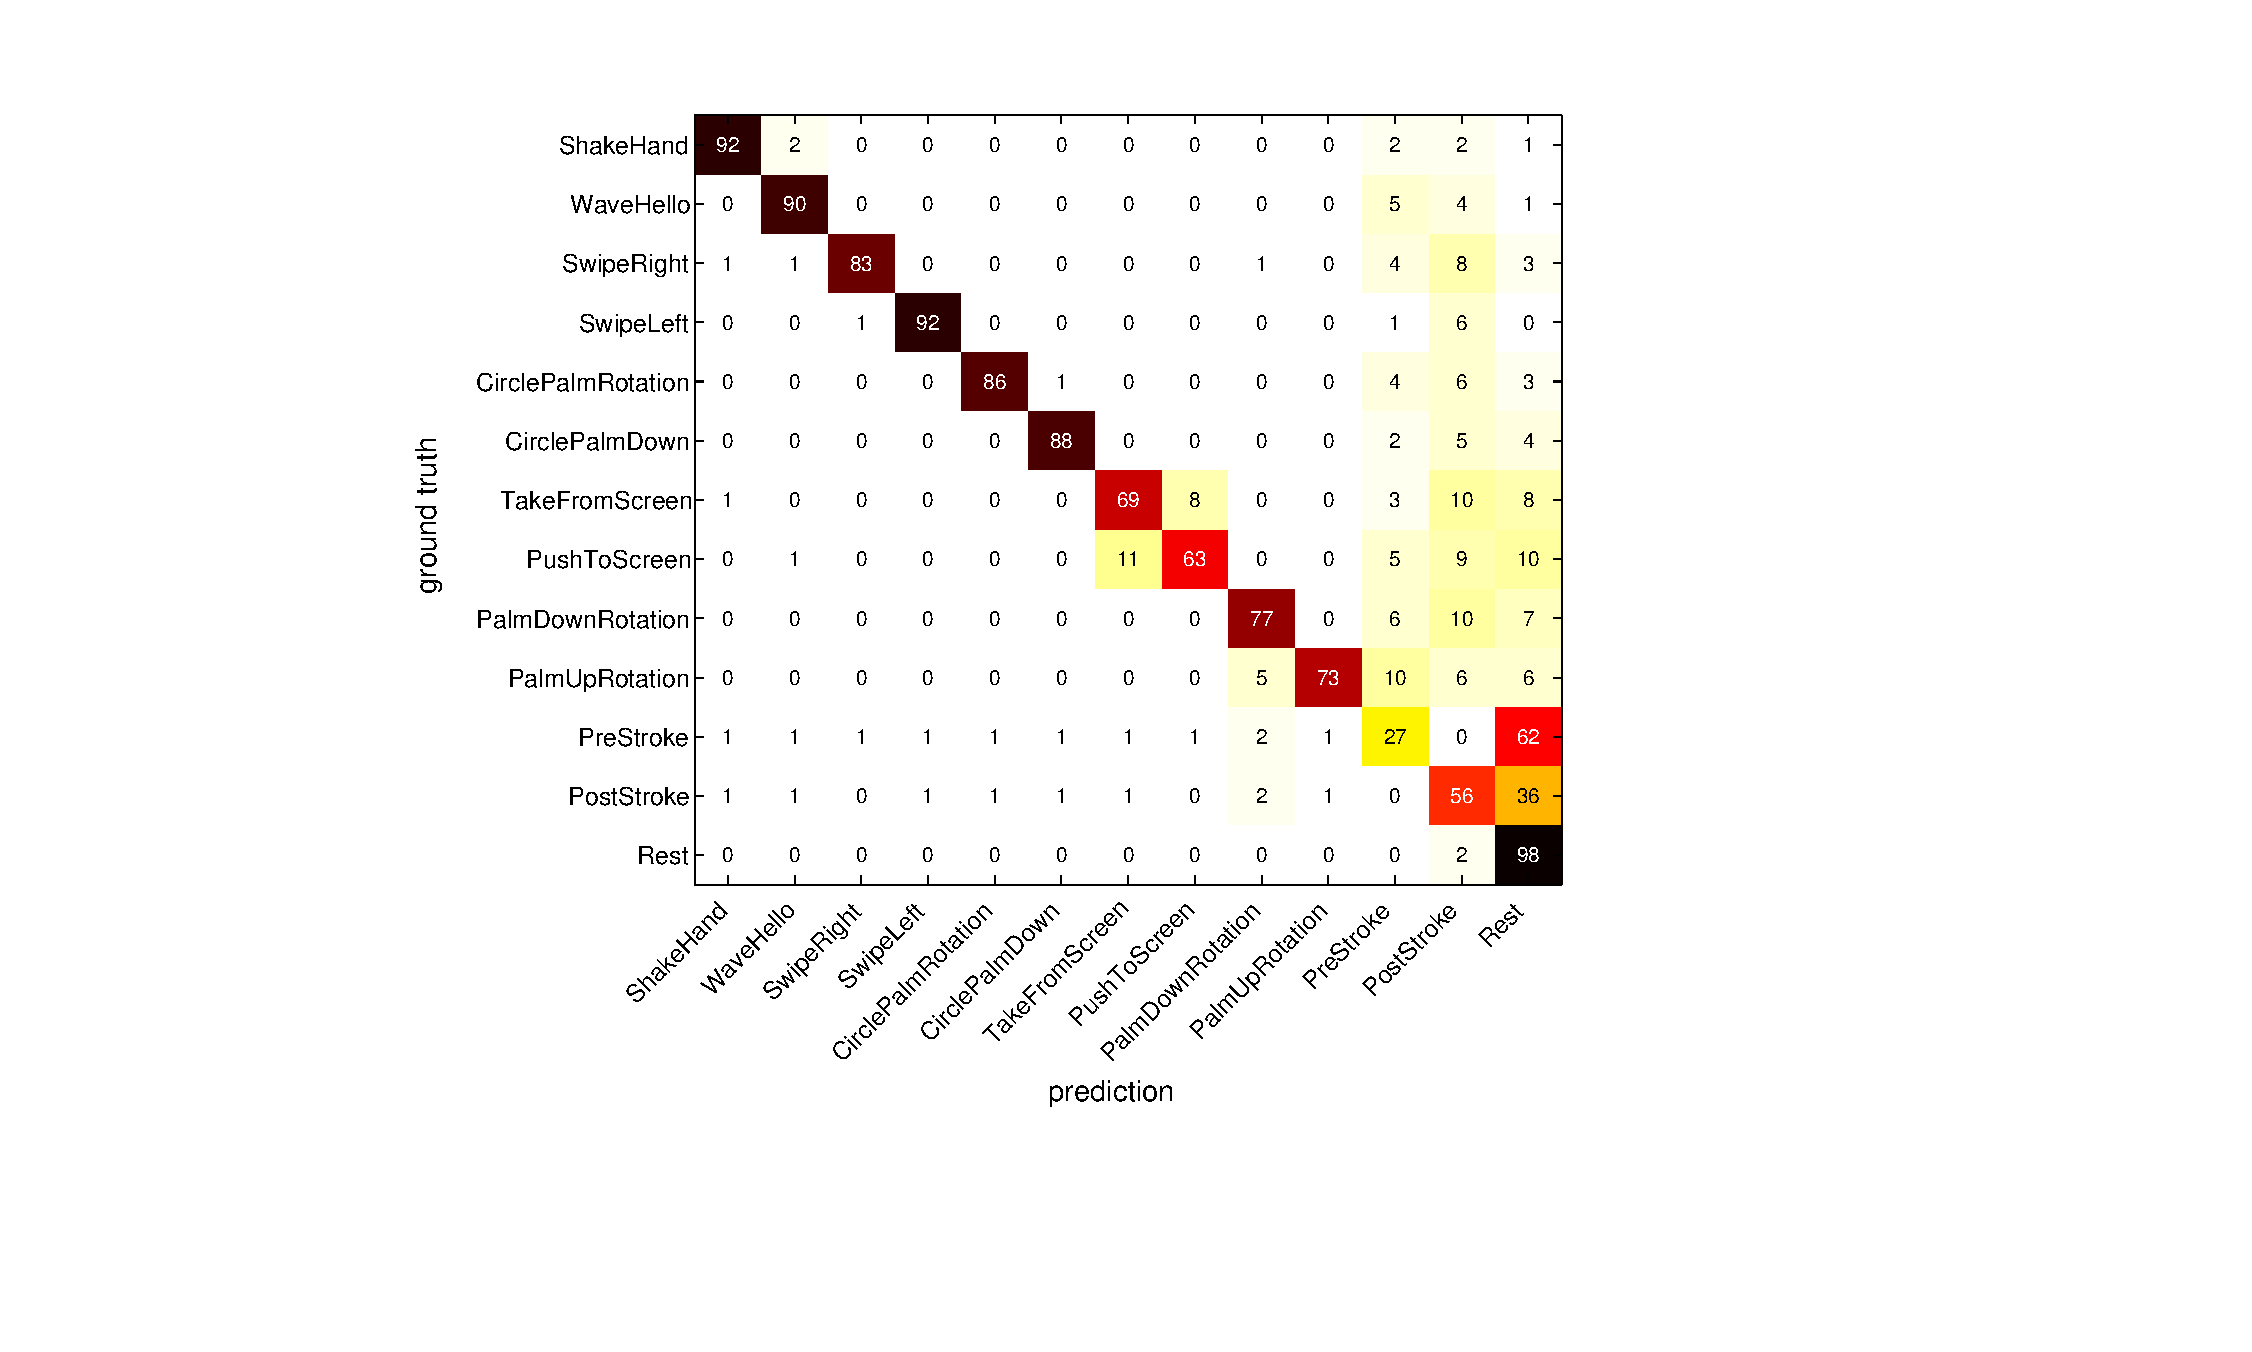
\includegraphics[trim={6cm 3.5cm 10cm 1.5cm}, clip,
width=0.9\columnwidth]{figures/confusion-matrix.eps} \caption{Per frame
classification confusion matrix based on result from 3-fold cross validation
using features computed form both the Kinect and IMU sensors. The numbers are
percentages.
The darker the color the higher the percentage.}
\label{fig:confusion}
\end{figure}

If no IMU is present, we can still compute velocity and acceleration from
relative positions, but we will lose the information on hand orientation which
is important do distinguish gestures with the same path but different hand
poses, e.g., gestures in the ChAirGest dataset.

It is useful to apply temporal smoothing on the motion data. In the
real-time system, I apply ``box'' smoothing (i.e., simple linear smoothing
with equal weights) with a window size of 15 frames on the relative positions of
the gesturing hand.

Figure~\ref{fig:motion-hist-rest} shows the histograms of the standardized $(x,
y, z)$ coordinates of relative position, velocity and acceleration from one user's
data in the YANG dataset. The peak values corresponds to the rest position
because it is the most frequent pose in the recording.
Figure~\ref{fig:motion-hist} shows the histogram of the same data excluding
those from the rest position. We can see that the distribution roughly follows
Gaussian or mixture of Gaussians distributions.

\begin{figure}[!tbh]
\centering
\subfigure[With rest positions.]{
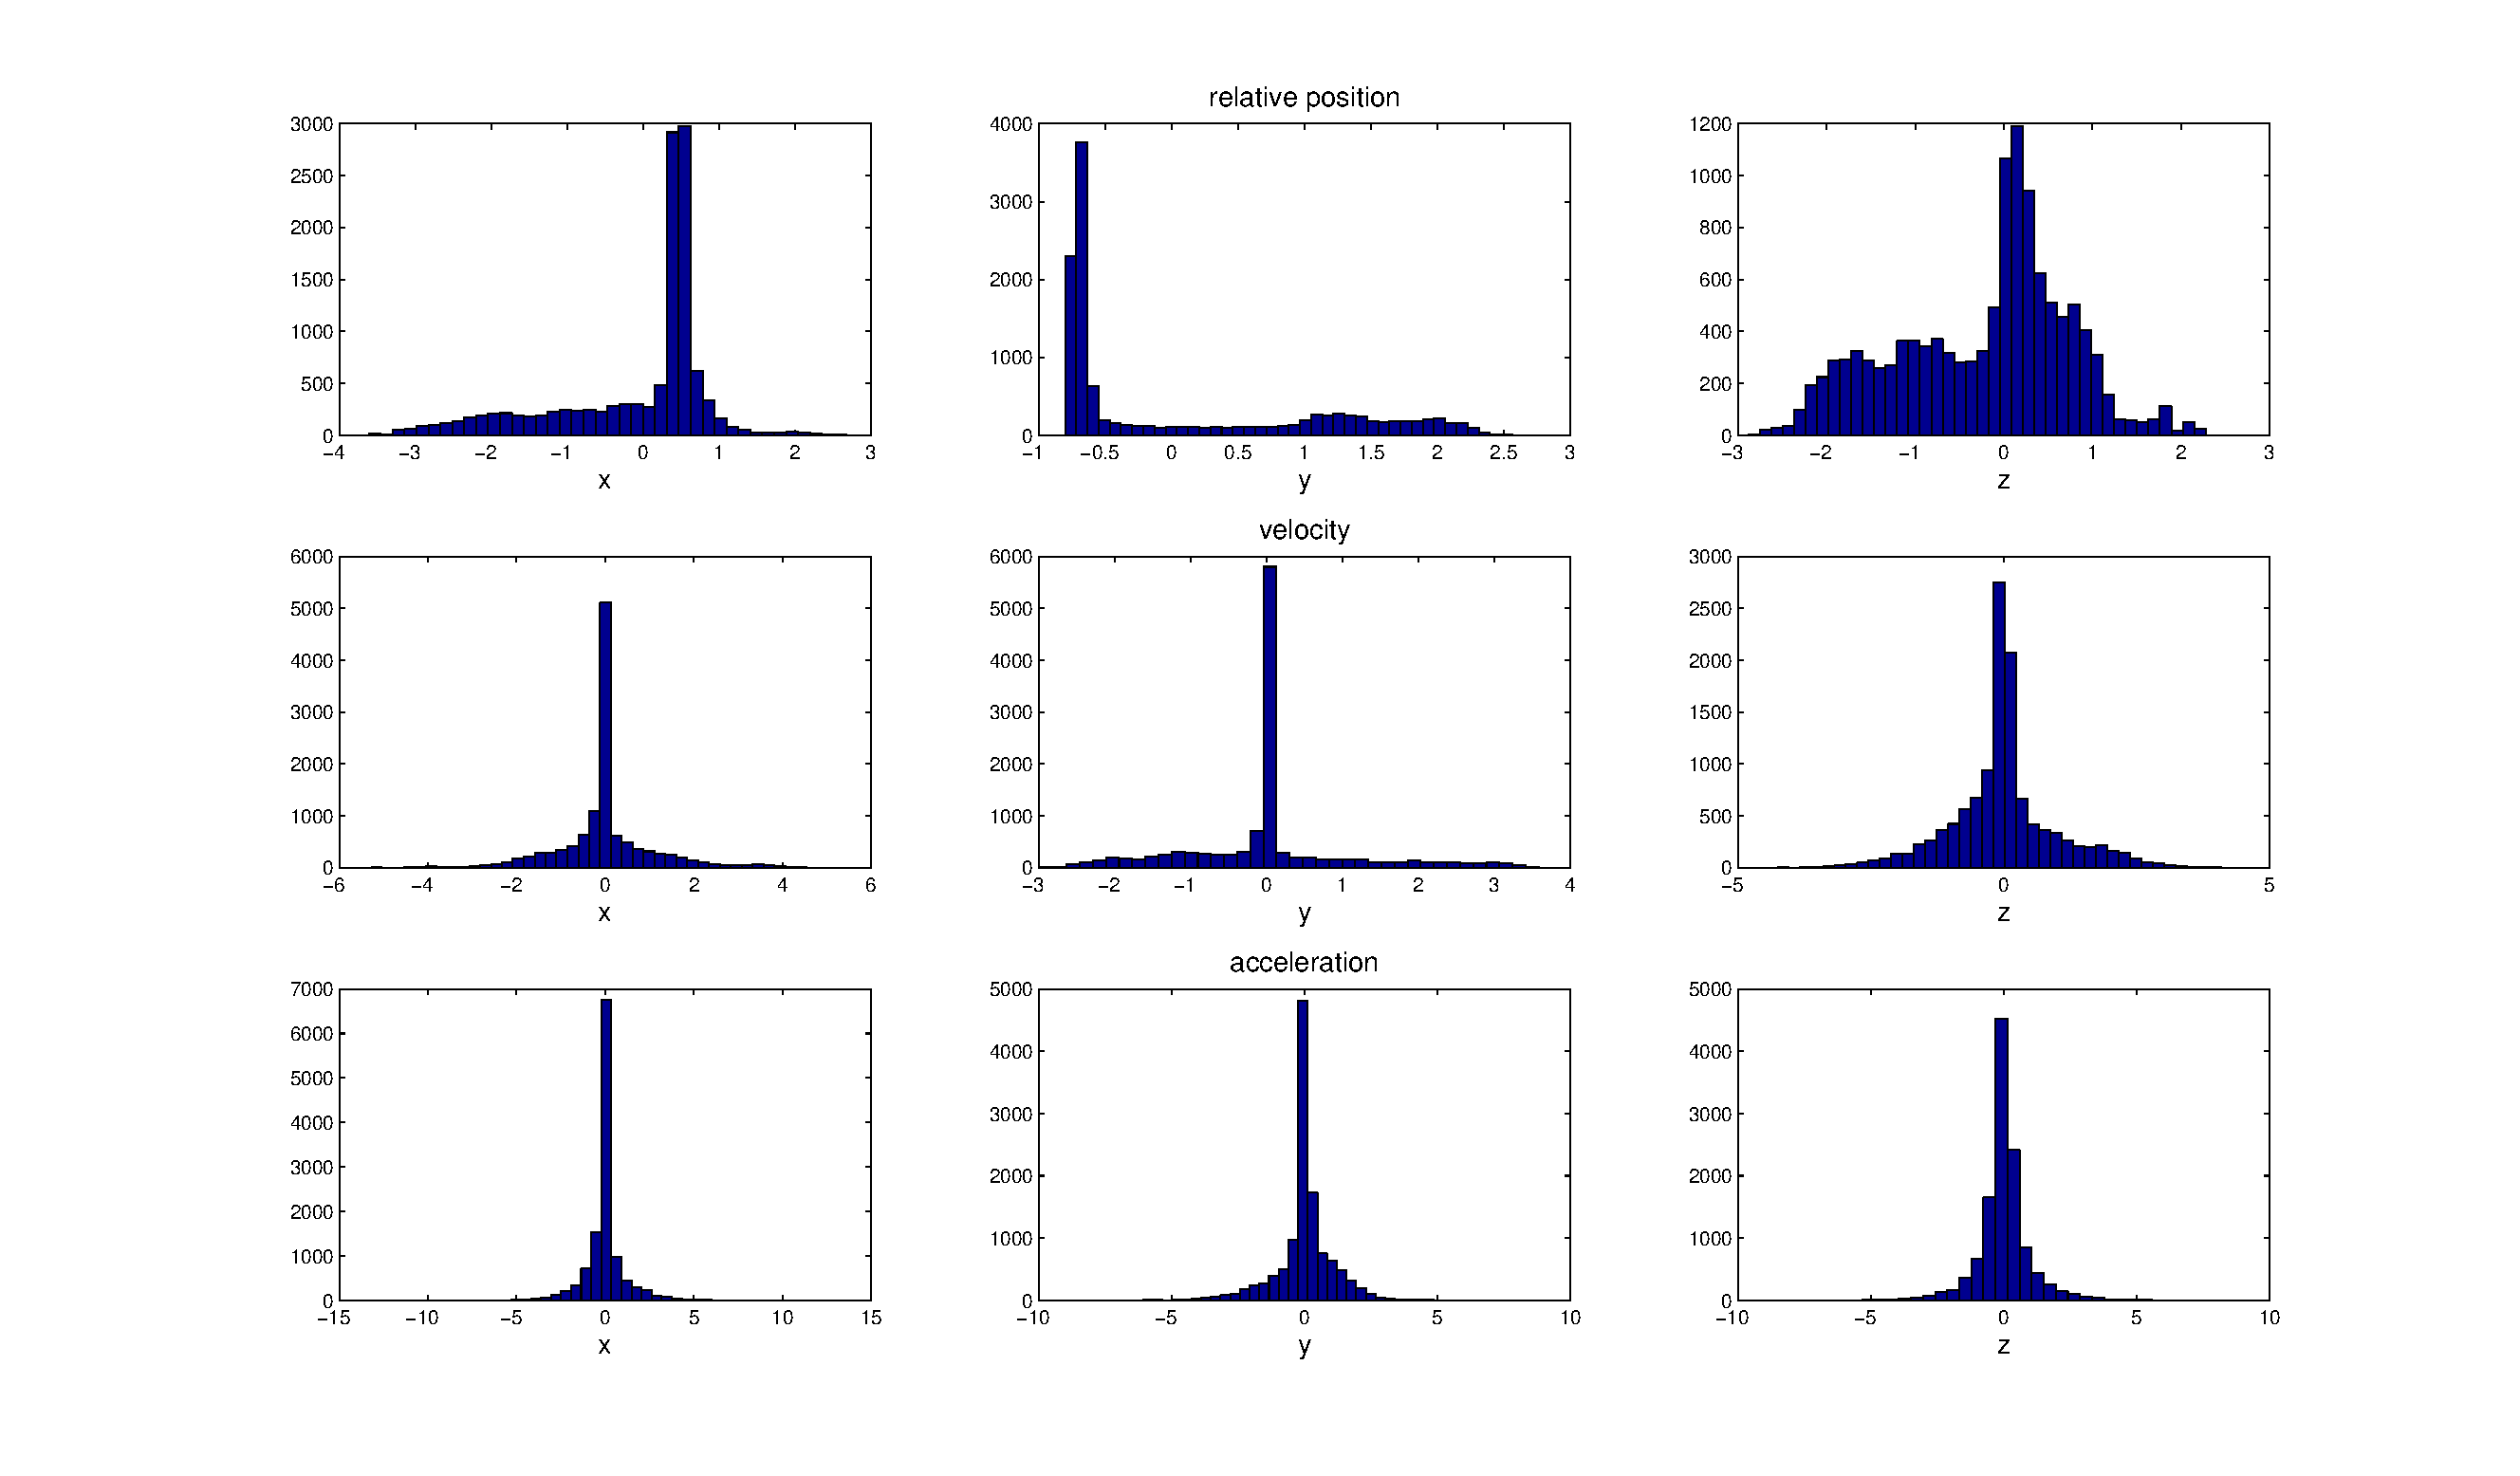
\includegraphics[trim=30mm 15mm 30mm 10mm,
clip, width=0.97\columnwidth]{figures/motion_hist_rest.eps}
\label{fig:motion-hist-rest}
}
\subfigure[Without rest positions.]{
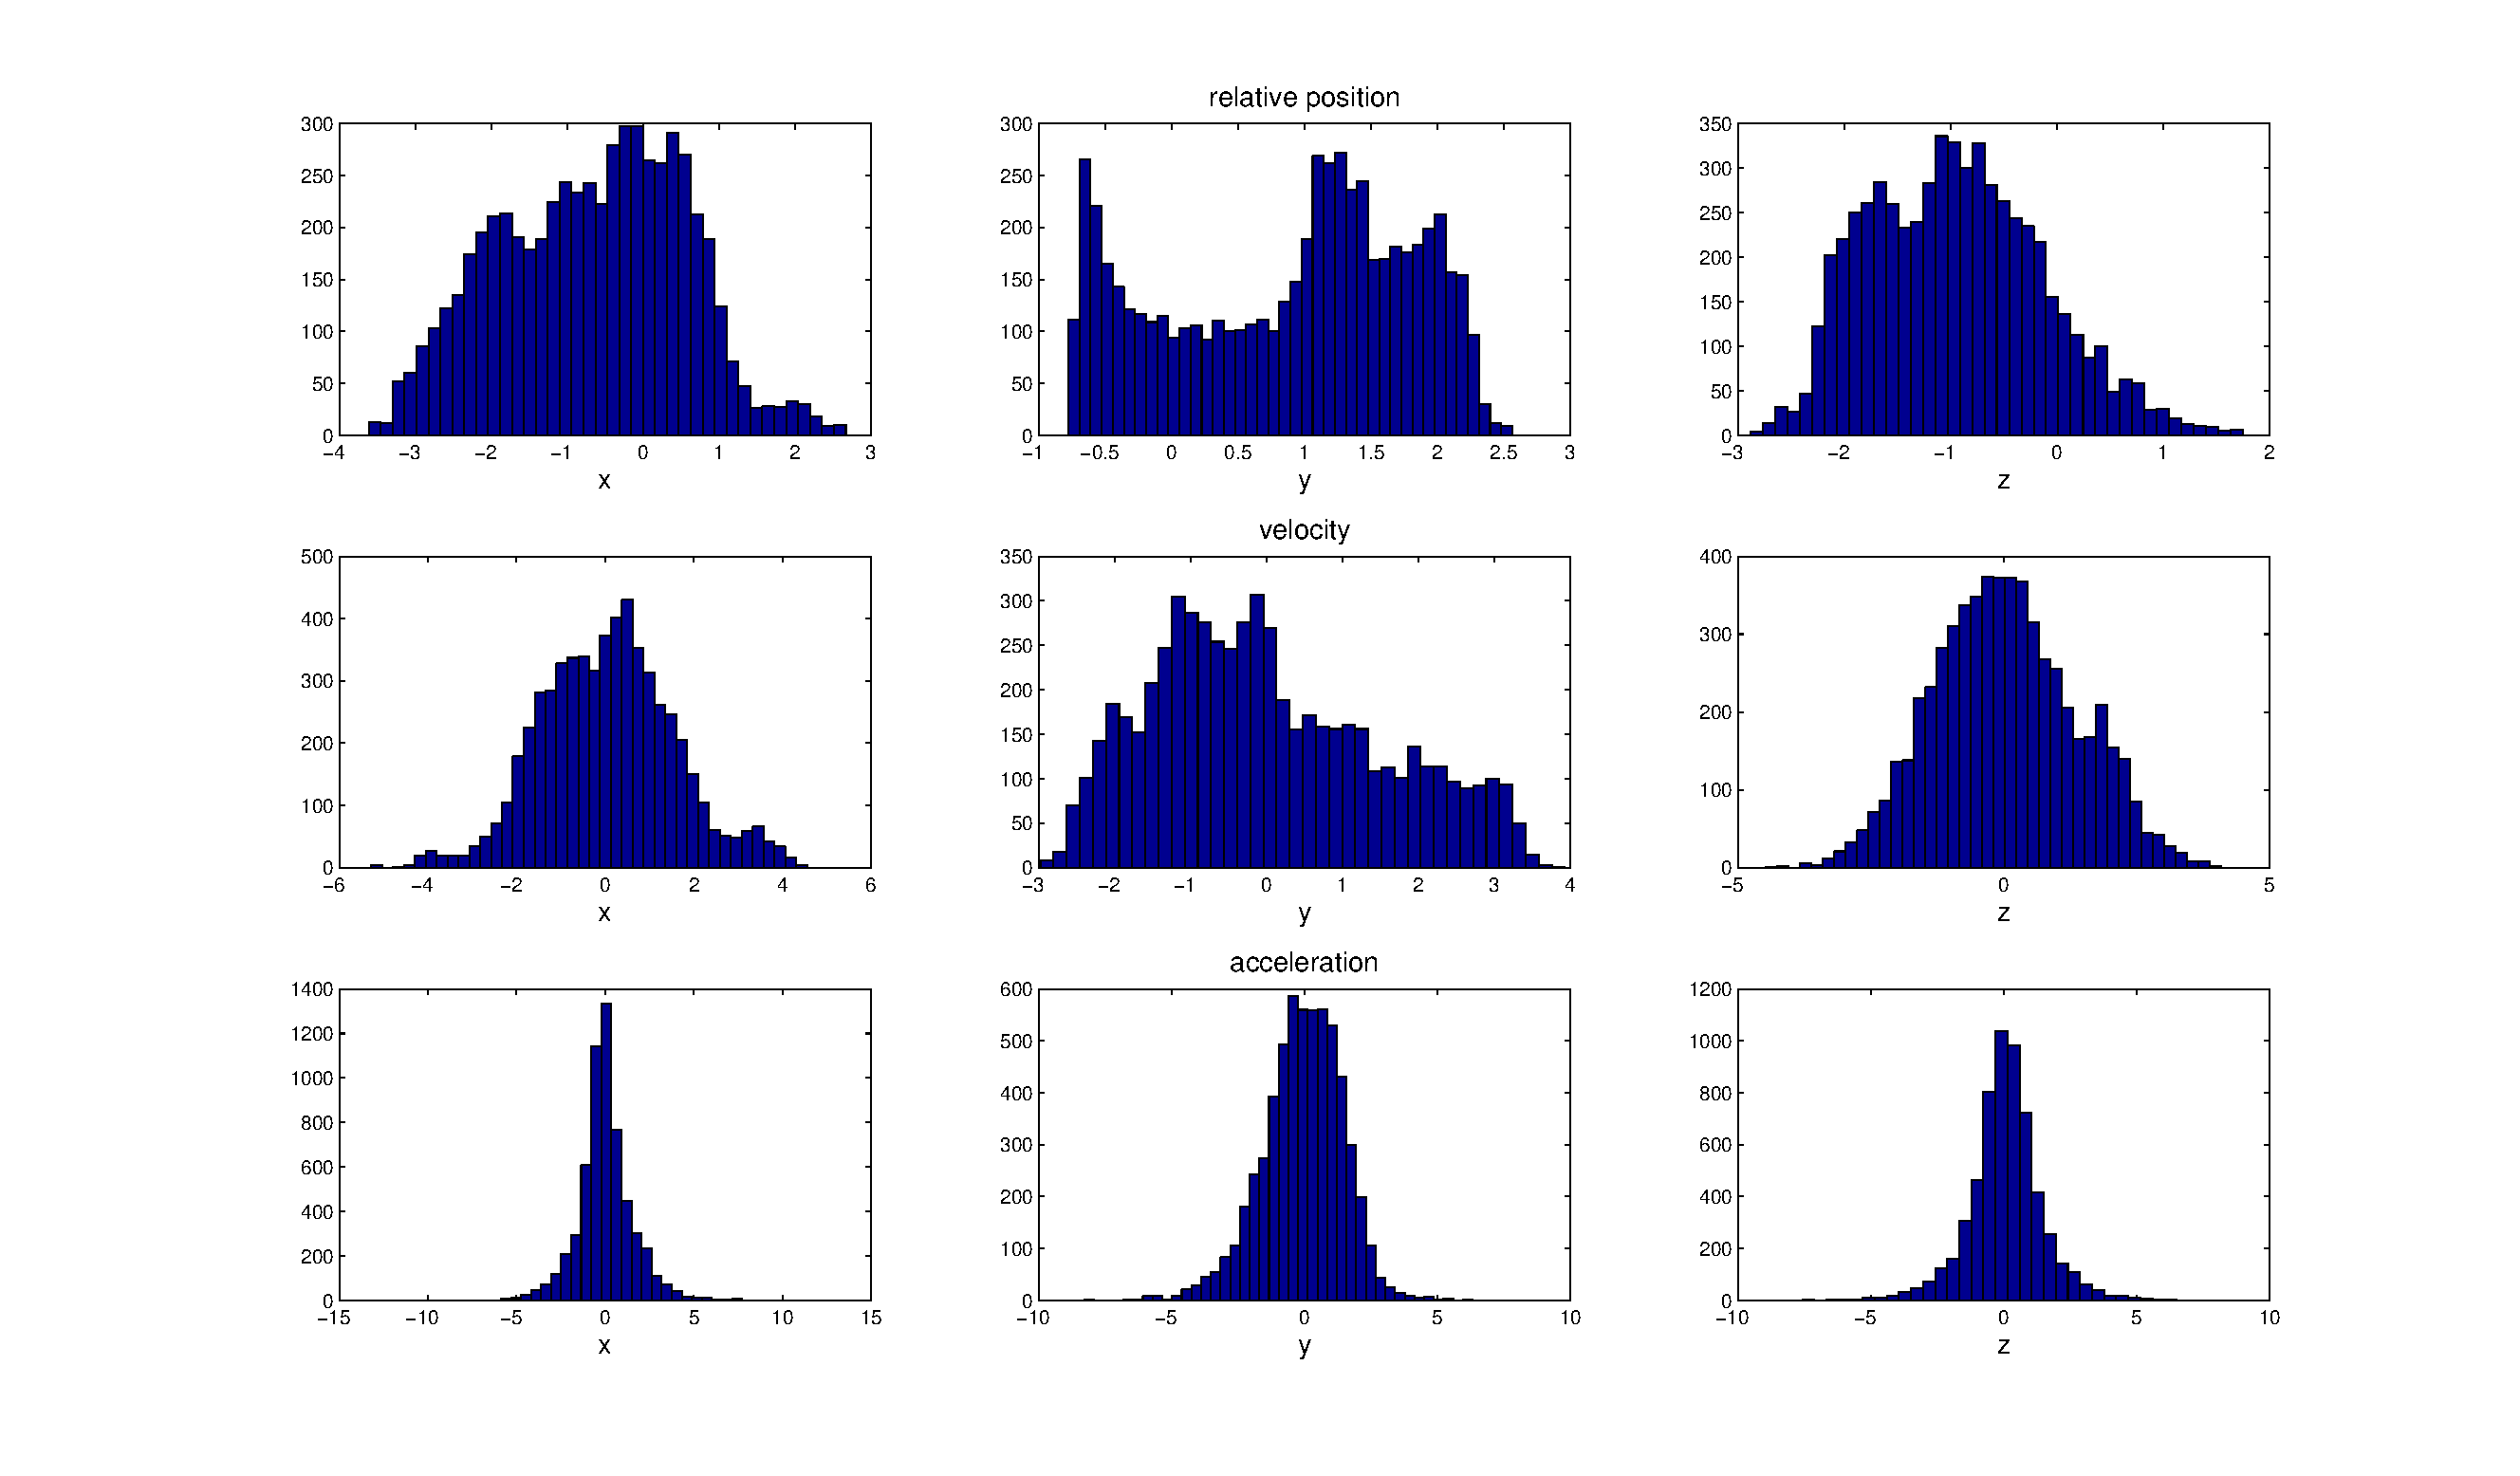
\includegraphics[trim=30mm 15mm 30mm 10mm,
clip, width=0.97\columnwidth]{figures/motion_hist.eps}
\label{fig:motion-hist}
}
\caption{Histograms of motion features.}
\end{figure}

%Try Xsens data on hand, quarternion.

\section{Hand Pose Features}
I use HOG as the feature descriptor for hand poses. The HOG feature descriptor
can be computed from either color, depth or both images. Figure~\ref{fig:hand}
shows sequences of hand image patches extracted using the salience based hand
tracking algorithm. The depth gray images are obtained by scaling the depth
values between 0 -- 255.

\begin{figure}[tbh]
  \centering
  \subfigure[Gray images converted from color images with only skin-colored
  pixels.] {
	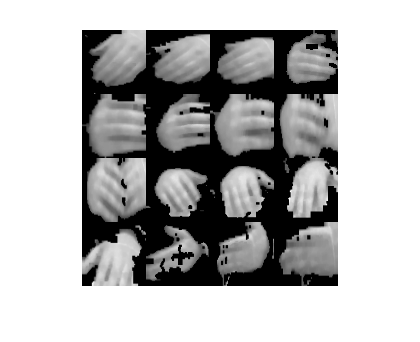
\includegraphics[width=0.45\textwidth]{figures/color_hand.png} 
  }
  \subfigure[Corresponding depth-mapped images.] {
  	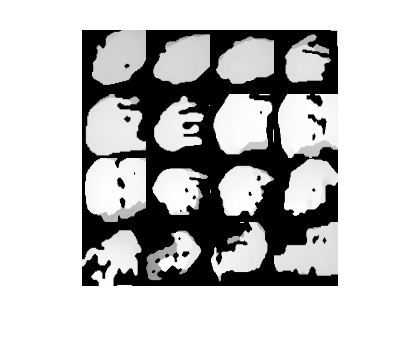
\includegraphics[width=0.45\textwidth]{figures/depth_hand.png}
  }
  \caption{$64\times64$px raw image patches of hands from the ChAirGest
  dataset.}
  \label{fig:hand}
\end{figure}

\subsection{Histogram of Oriented Gradients (HOG)}
For each pixel, the magnitude ($r$) and the orientation ($\theta$) of the
gradient are
\begin{align*}
r &= \sqrt{dx^2 + dy^2} \\
\theta &= \text{arccos}(dx / r) 
\end{align*}
where $dx$ and $dy$ are computed using a centered $[-1, 0, 1]$ derivative mask.
Each pixel contributes a weighted vote (the magnitude of the gradient $r$) to an
edge orientation histogram based on the orientation, $\theta$, of the gradient
element centered on it, and the votes are accumulated into orientation bins over local spatial regions called
\textit{cells}.
The orientation bins are evenly spaced over 0\textdegree -- 180\textdegree
(``unsigned'' gradient). To reduce aliasing, votes are interpolated
bilinearly between the neighboring bin centers in both orientation and
position~\cite{dalal05}. 

Fine orientation and spatial binning turns out to be essential for good
performance. My evaluation shows that using $4\times 4$px cells
(\texttt{cell\_size} = 4) and 9 orientation bins gives the best result.

Finally, cell values are normalized using blocks of $2\times 2$ cells
(Figure~\ref{fig:cell}).
If an image $I$ has dimensions $m\times n$, the size of the computed feature vector
$H$ is $(m/\texttt{cell\_size} - 1) \times (n/\texttt{cell\_size} - 1) \times
\texttt{num\_bin}$. Figure~\ref{fig:hand-hog} hows a visualization of the HOG
descriptors from both the color images and depth-mapped images.

\begin{figure}[!tbh]
\centering
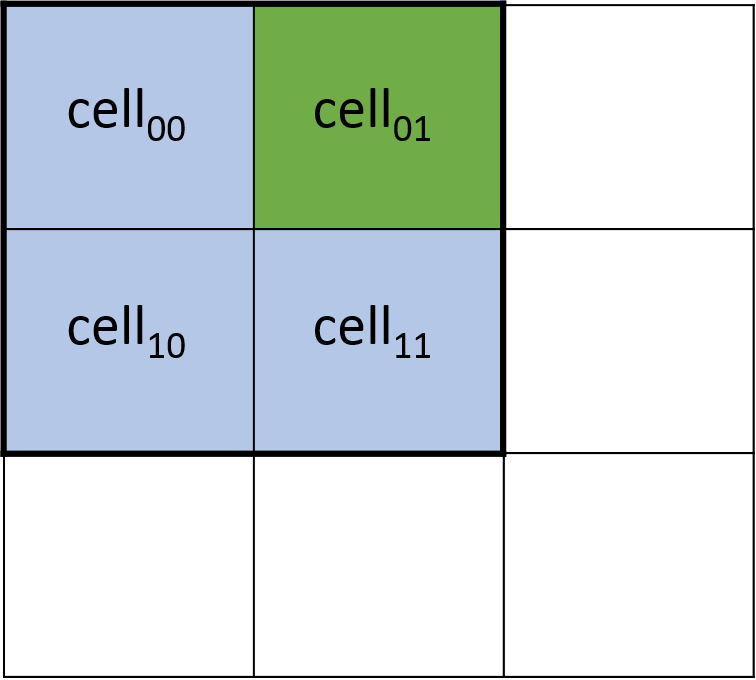
\includegraphics[width=0.3\textwidth]{figures/cell.png}
\caption{Histogram values in $\text{cell}_{01}$ is normalized by the sum in
$\text{cell}_{00}$, $\text{cell}_{01}$, $\text{cell}_{10}$,
and $\text{cell}_{11}$.
}
\label{fig:cell}
\end{figure}

\begin{figure}[!tbh]
  \centering
  \subfigure[Gray images converted from color images.] {
  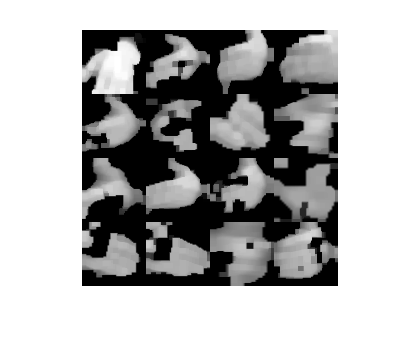
\includegraphics[trim=10mm 15mm 10mm 5mm,
clip,width=0.45\textwidth]{figures/color_denoised_5.png} 
  }
  \subfigure[Corresponding depth-mapped images.] {
    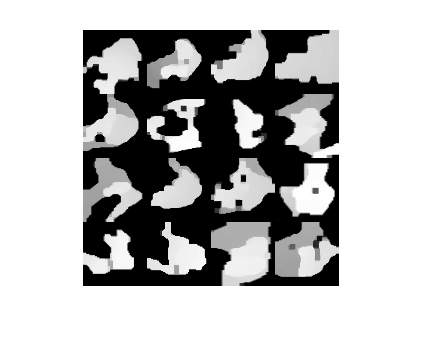
\includegraphics[trim=10mm 15mm 10mm 5mm,
clip,width=0.45\textwidth]{figures/depth_denoised_5.png}
  }
  \subfigure[HOG from color images (converted to gray).] {
  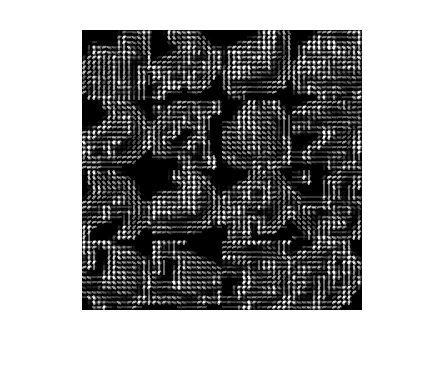
\includegraphics[trim=2mm 15mm 13mm 0mm,
clip,width=0.45\textwidth]{figures/color_hog.png} }
  \subfigure[HOG from depth-mapped images.] {
    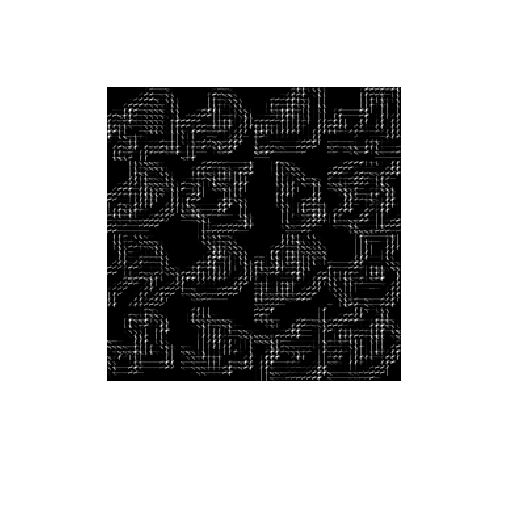
\includegraphics[trim={7mm 35mm 11mm 0cm},
  clip, width=0.5\textwidth]{figures/depth_hog.png}
  }
  \caption{Visualization of HOG descriptors computed from $64\times64$px
  image patches.}
  \label{fig:hand-hog}
\end{figure}

\subsection{Compare HOG from Color or Depth Images}
Using the ChAirGest dataset and the same recognition method, I compared
results using HOG computed from different types of
data. Table~\ref{tab:comp-feature} shows that
using HOG from both color and depth data gives the highest $F_1$ score. However, the improvement is small
compared with using HOG computed from depth data only. As a result, in the
real-time system, I only use HOG computed from depth data to increase
processing speed.

\begin{table}[tbh]
\begin{center}
\begin{tabular}{|l|p{2cm}|p{2cm}|p{1.7cm}|p{2cm}|}
\hline
          & \thead{motion (no orientation)} & \thead{color} & \thead{depth} &
          \thead{color and depth}
          \\
\hline
$F_1$ Score & 0.677 (0.04) & 0.703 (0.01) & 0.720 (0.02) & \textbf{0.723} (0.01)
\\
\hline
ATSR Score & \textbf{0.893} (0.02) & 0.870 (0.01) & 0.880 (0.01) & 0.873 (0.01)
\\
\hline
Final Score & 0.710 (0.03) & 0.732 (0.01) & 0.748 (0.01) & \textbf{0.749} (0.00)
\\
\hline
\end{tabular}
\caption{Comparison of the average 3-fold cross validation results for
features computed from the Kinect sensor data using the ChAirGest dataset.
Values in parentheses are standard deviations.}
\label{tab:comp-feature}
\end{center}
\end{table}

The reason that HOG from depth data gives better result than HOG from color data
could be that depth data contains more information about the contour the hand in
one more dimension (see Figure~\ref{fig:hand-3d}).
 
\begin{figure}[tbh]
\centering
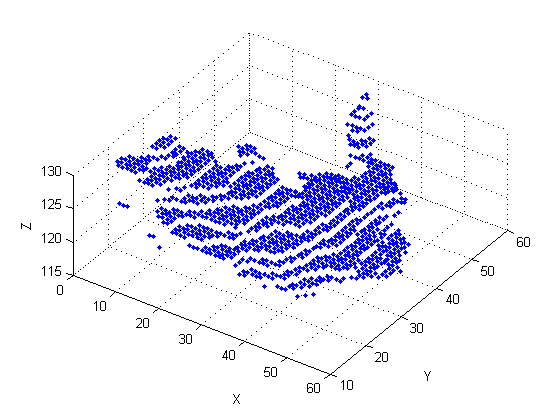
\includegraphics[width=0.5\textwidth]{figures/hand3d.png}
\caption{View of quantized depth data of a hand in 3D.}
\label{fig:hand-3d}
\end{figure}

The confusion matrices in Figure~\ref{fig:confusion2} shows that ``Take
from Screen'' and ``Push to Screen'' have the lowest recognition accuracy,
especially when using the Kinect data. I notice that, in this dataset, when the
users extend their hands towards the screen, the hands are too close to the sensor (below the too near range), and the depth sensor cannot get accurate readings.

Table~\ref{tab:comp-feature} also indicates that if we only use motion features
such as relative position, velocity and acceleration, the result is poor because it cannot distinguish gestures with
the same path but different hand postures such as ``Wave Hello'' and ``Shake
Hand'', ``Circle Palm Rotation'' and ``Circle Palm Down''
(Figure~\ref{fig:confusion-motion}). However, using motion features only gives
the highest temporal gesture nucleus segmentation score (the ATSR score). This
means that for segmentation, motion features are probably more useful than the
hand pose features.

\begin{figure}[!hp]
\centering
\subfigure[Using HOG computed from both color and depth data.]{
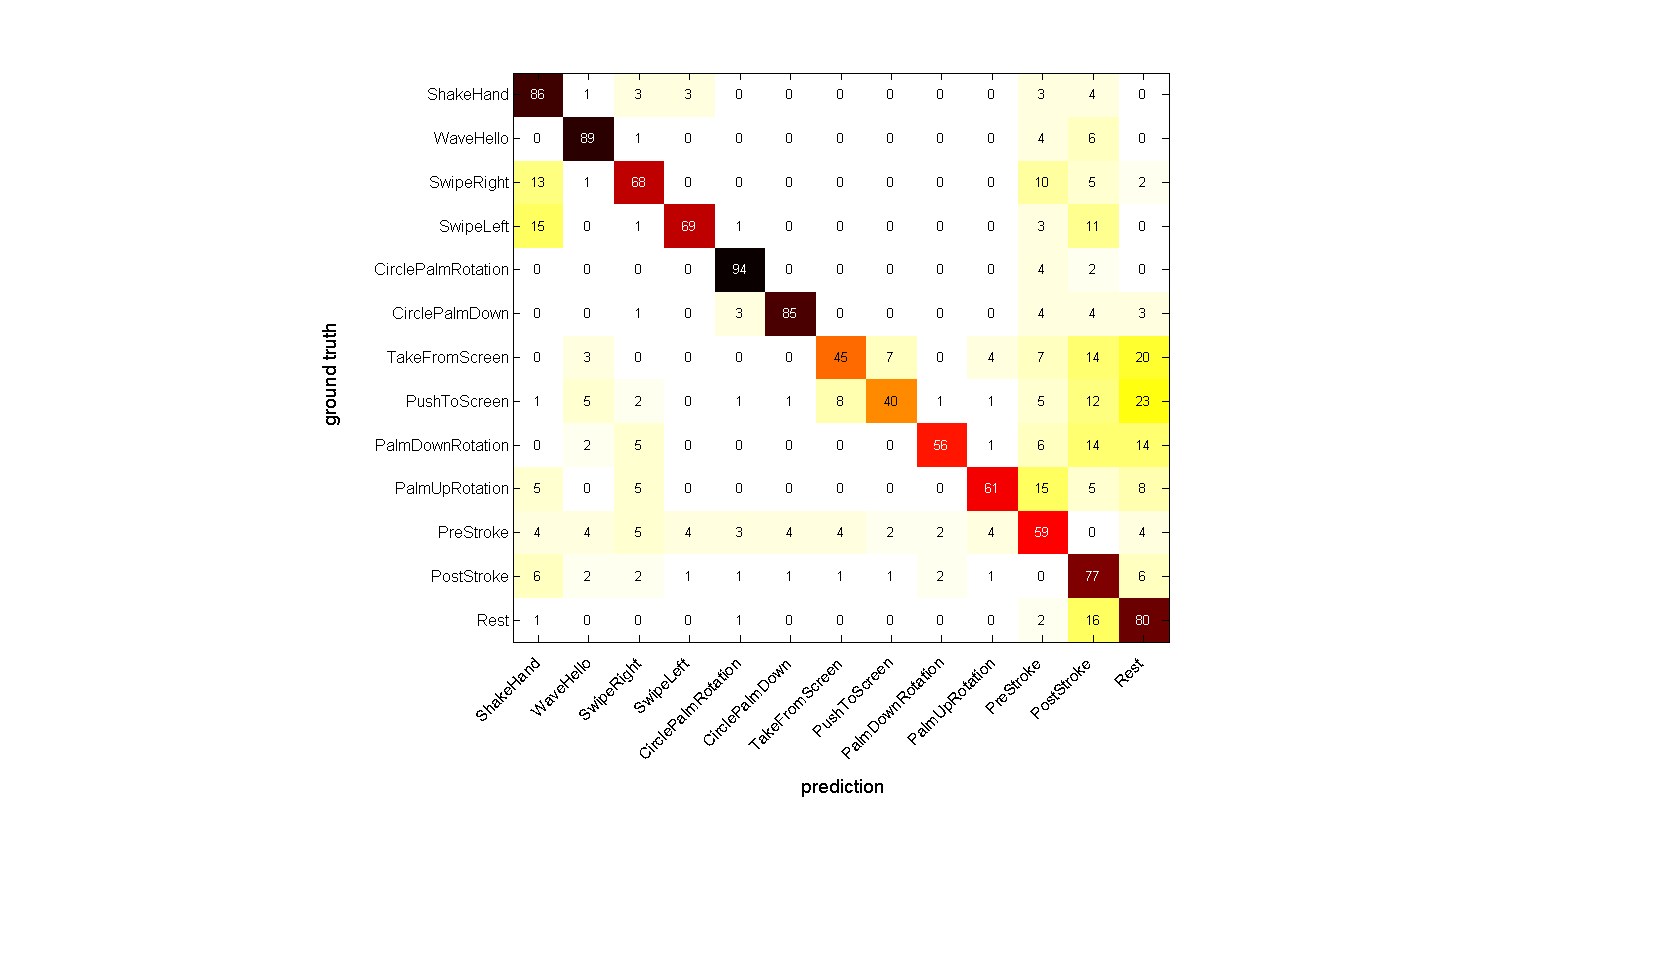
\includegraphics[trim={8.5cm 4.5cm 12cm 1.5cm}, clip,
width=0.7\columnwidth]{figures/confusion_color_depth.png}
\label{fig:confusion-color-depth} }
\subfigure[Using motion features only (relative position, velocity,
acceleration)]{ 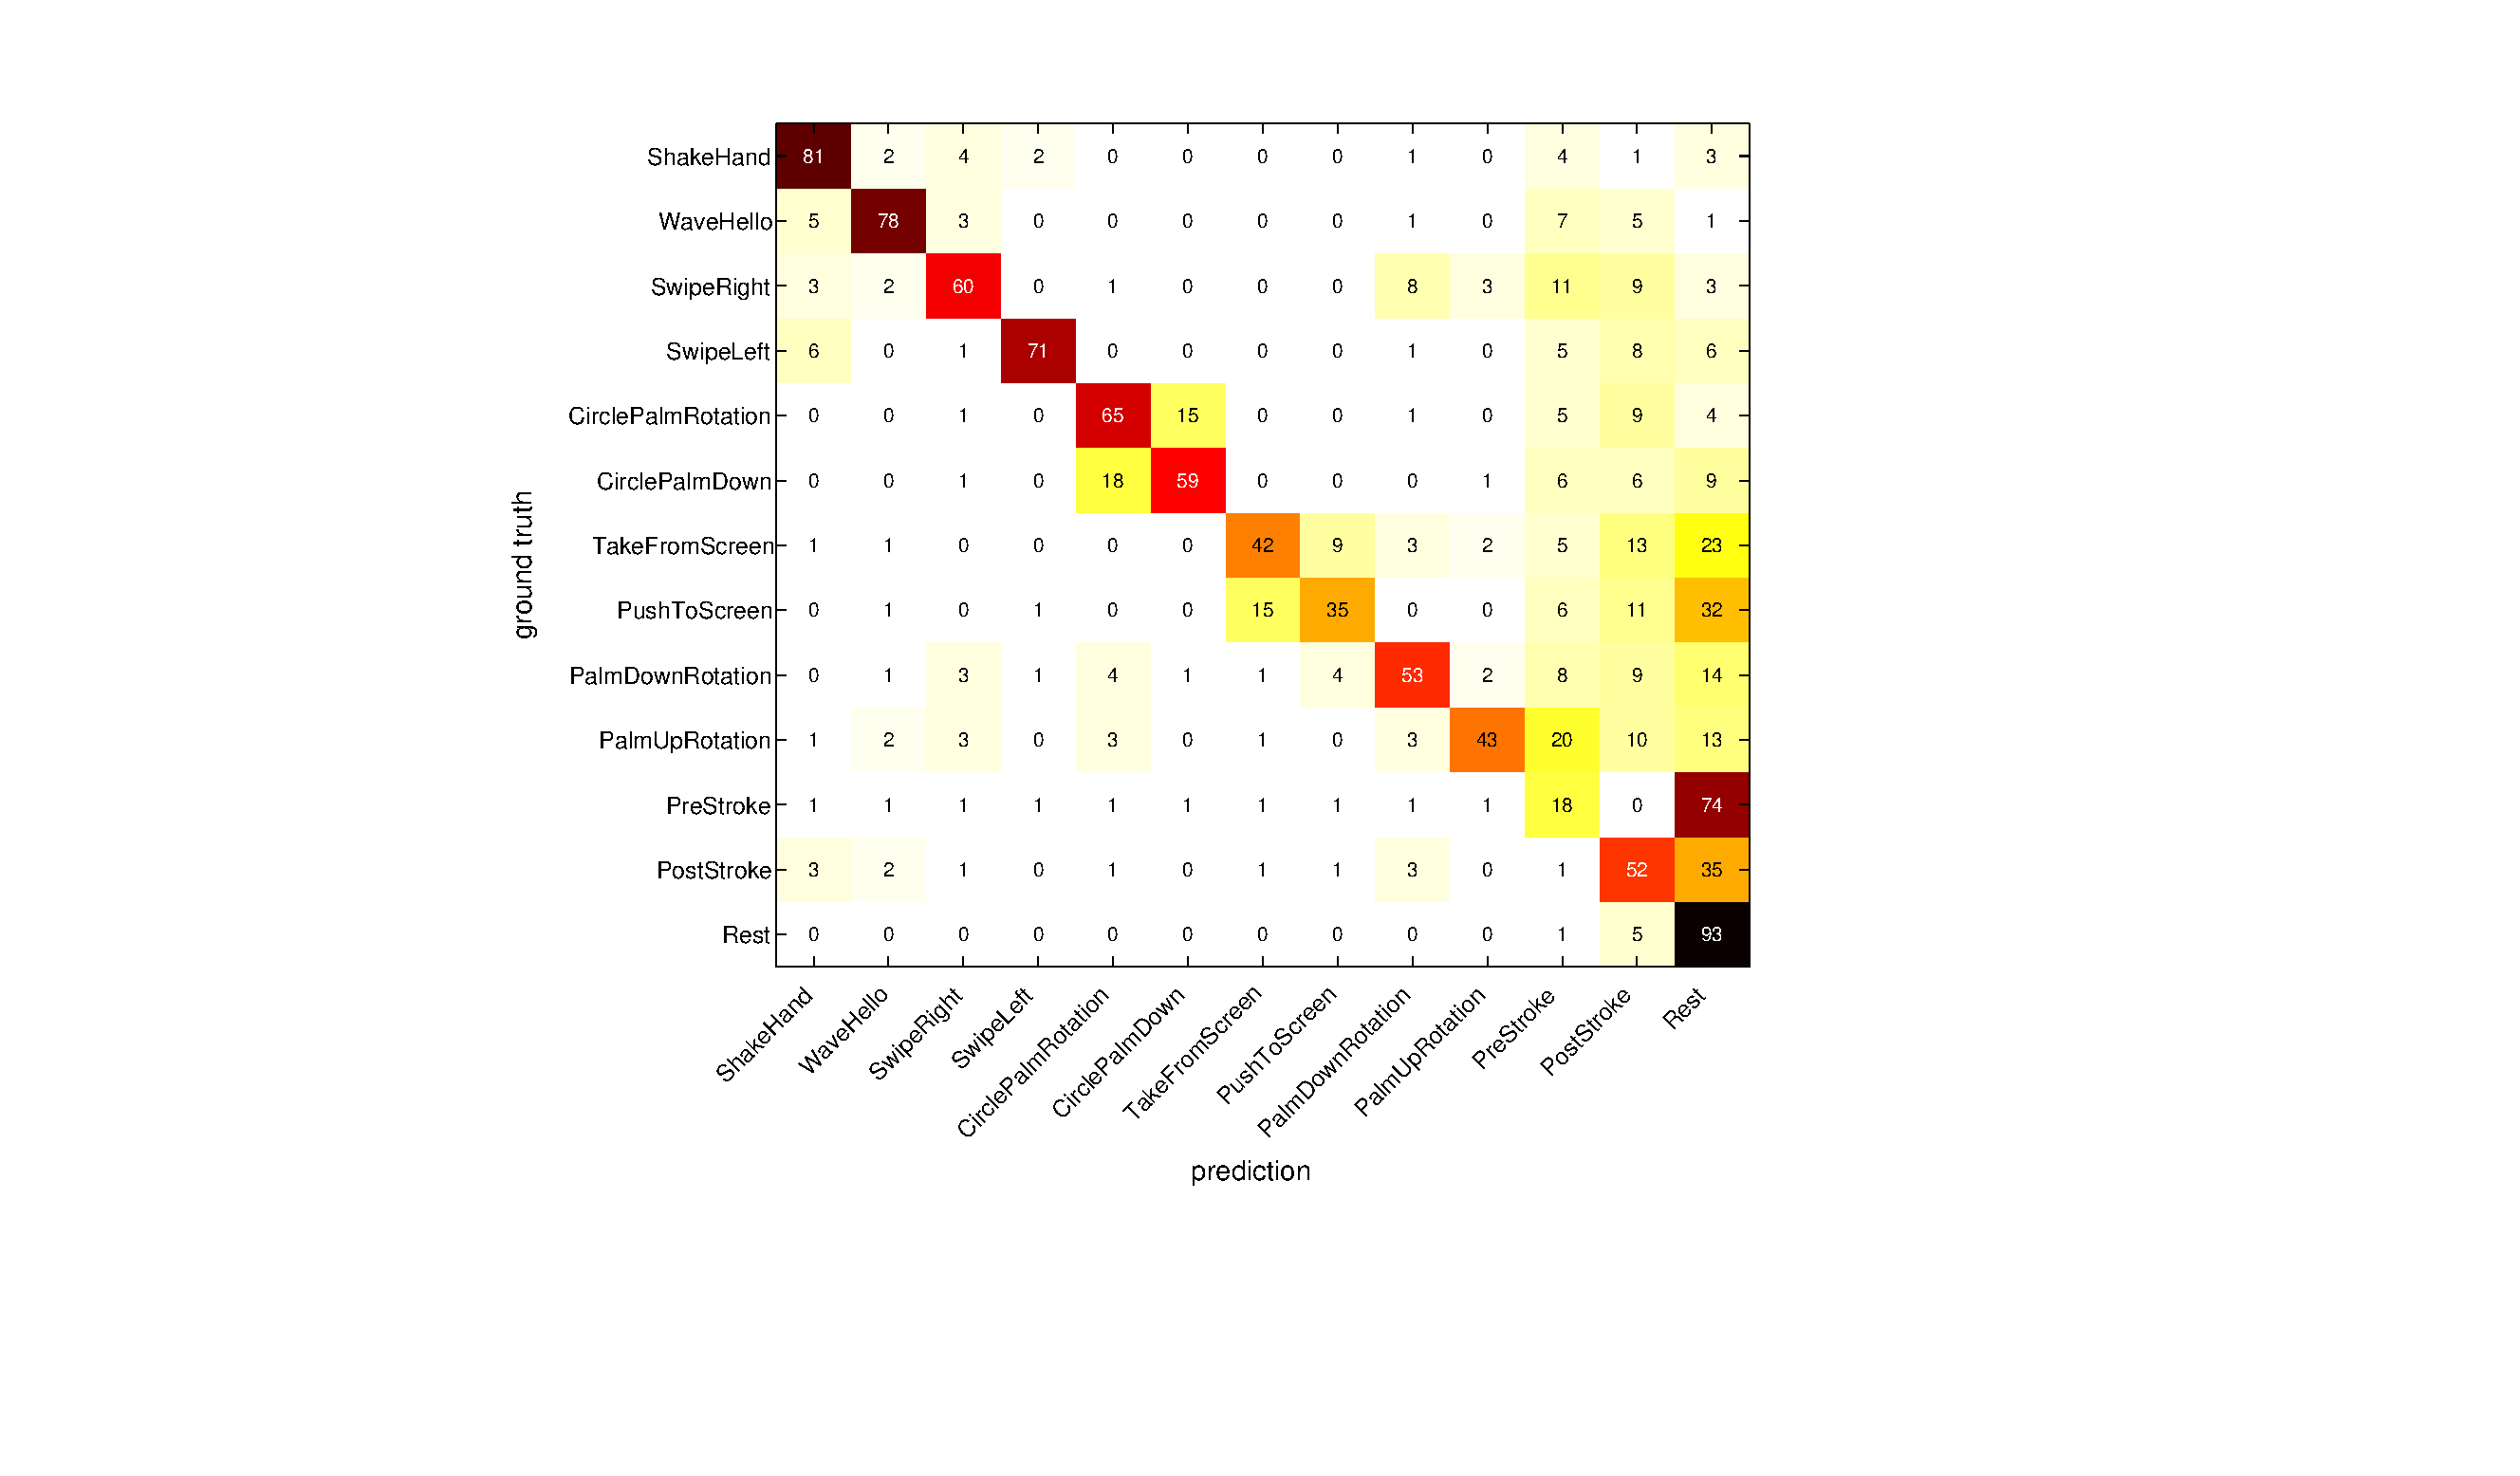
\includegraphics[trim={8.5cm 4.5cm 12cm 1.5cm}, clip,
width=0.7\columnwidth]{figures/confusion_motion.eps}\label{fig:confusion-motion}
}
\caption{Per frame
classification confusion matrices based on result from 3-fold cross validation
using the ChAirGest dataset. The numbers are percentages. The darker
the color the higher the percentage.}
\label{fig:confusion2}
\end{figure}

\section{Principal Component Analysis}
The dimension of the HOG feature descriptor can be large, therefore, I use
Principal Component Analysis (PCA)~\cite{pca} to reduce its dimensionality (see
Appendix~\ref{app:pca} for detail). PCA can be seen as a feature
encoder~\cite{ranzato07}.

The number of principal components is determined through cross-validation. For
the YANG dataset, I use 15 principal components from the HOG feature descriptor.
We use one user's data from the YANG dataset to visualize the PCA
encoded HOG descriptors. Figure~\ref{fig:pca} shows the histograms of the 15
variables after projecting the original HOG descriptors onto the principal
components and then applying standardization.
We observe that the distributions closely follow Gaussian or mixture of
Gaussians distributions.

\begin{figure}[tbh]
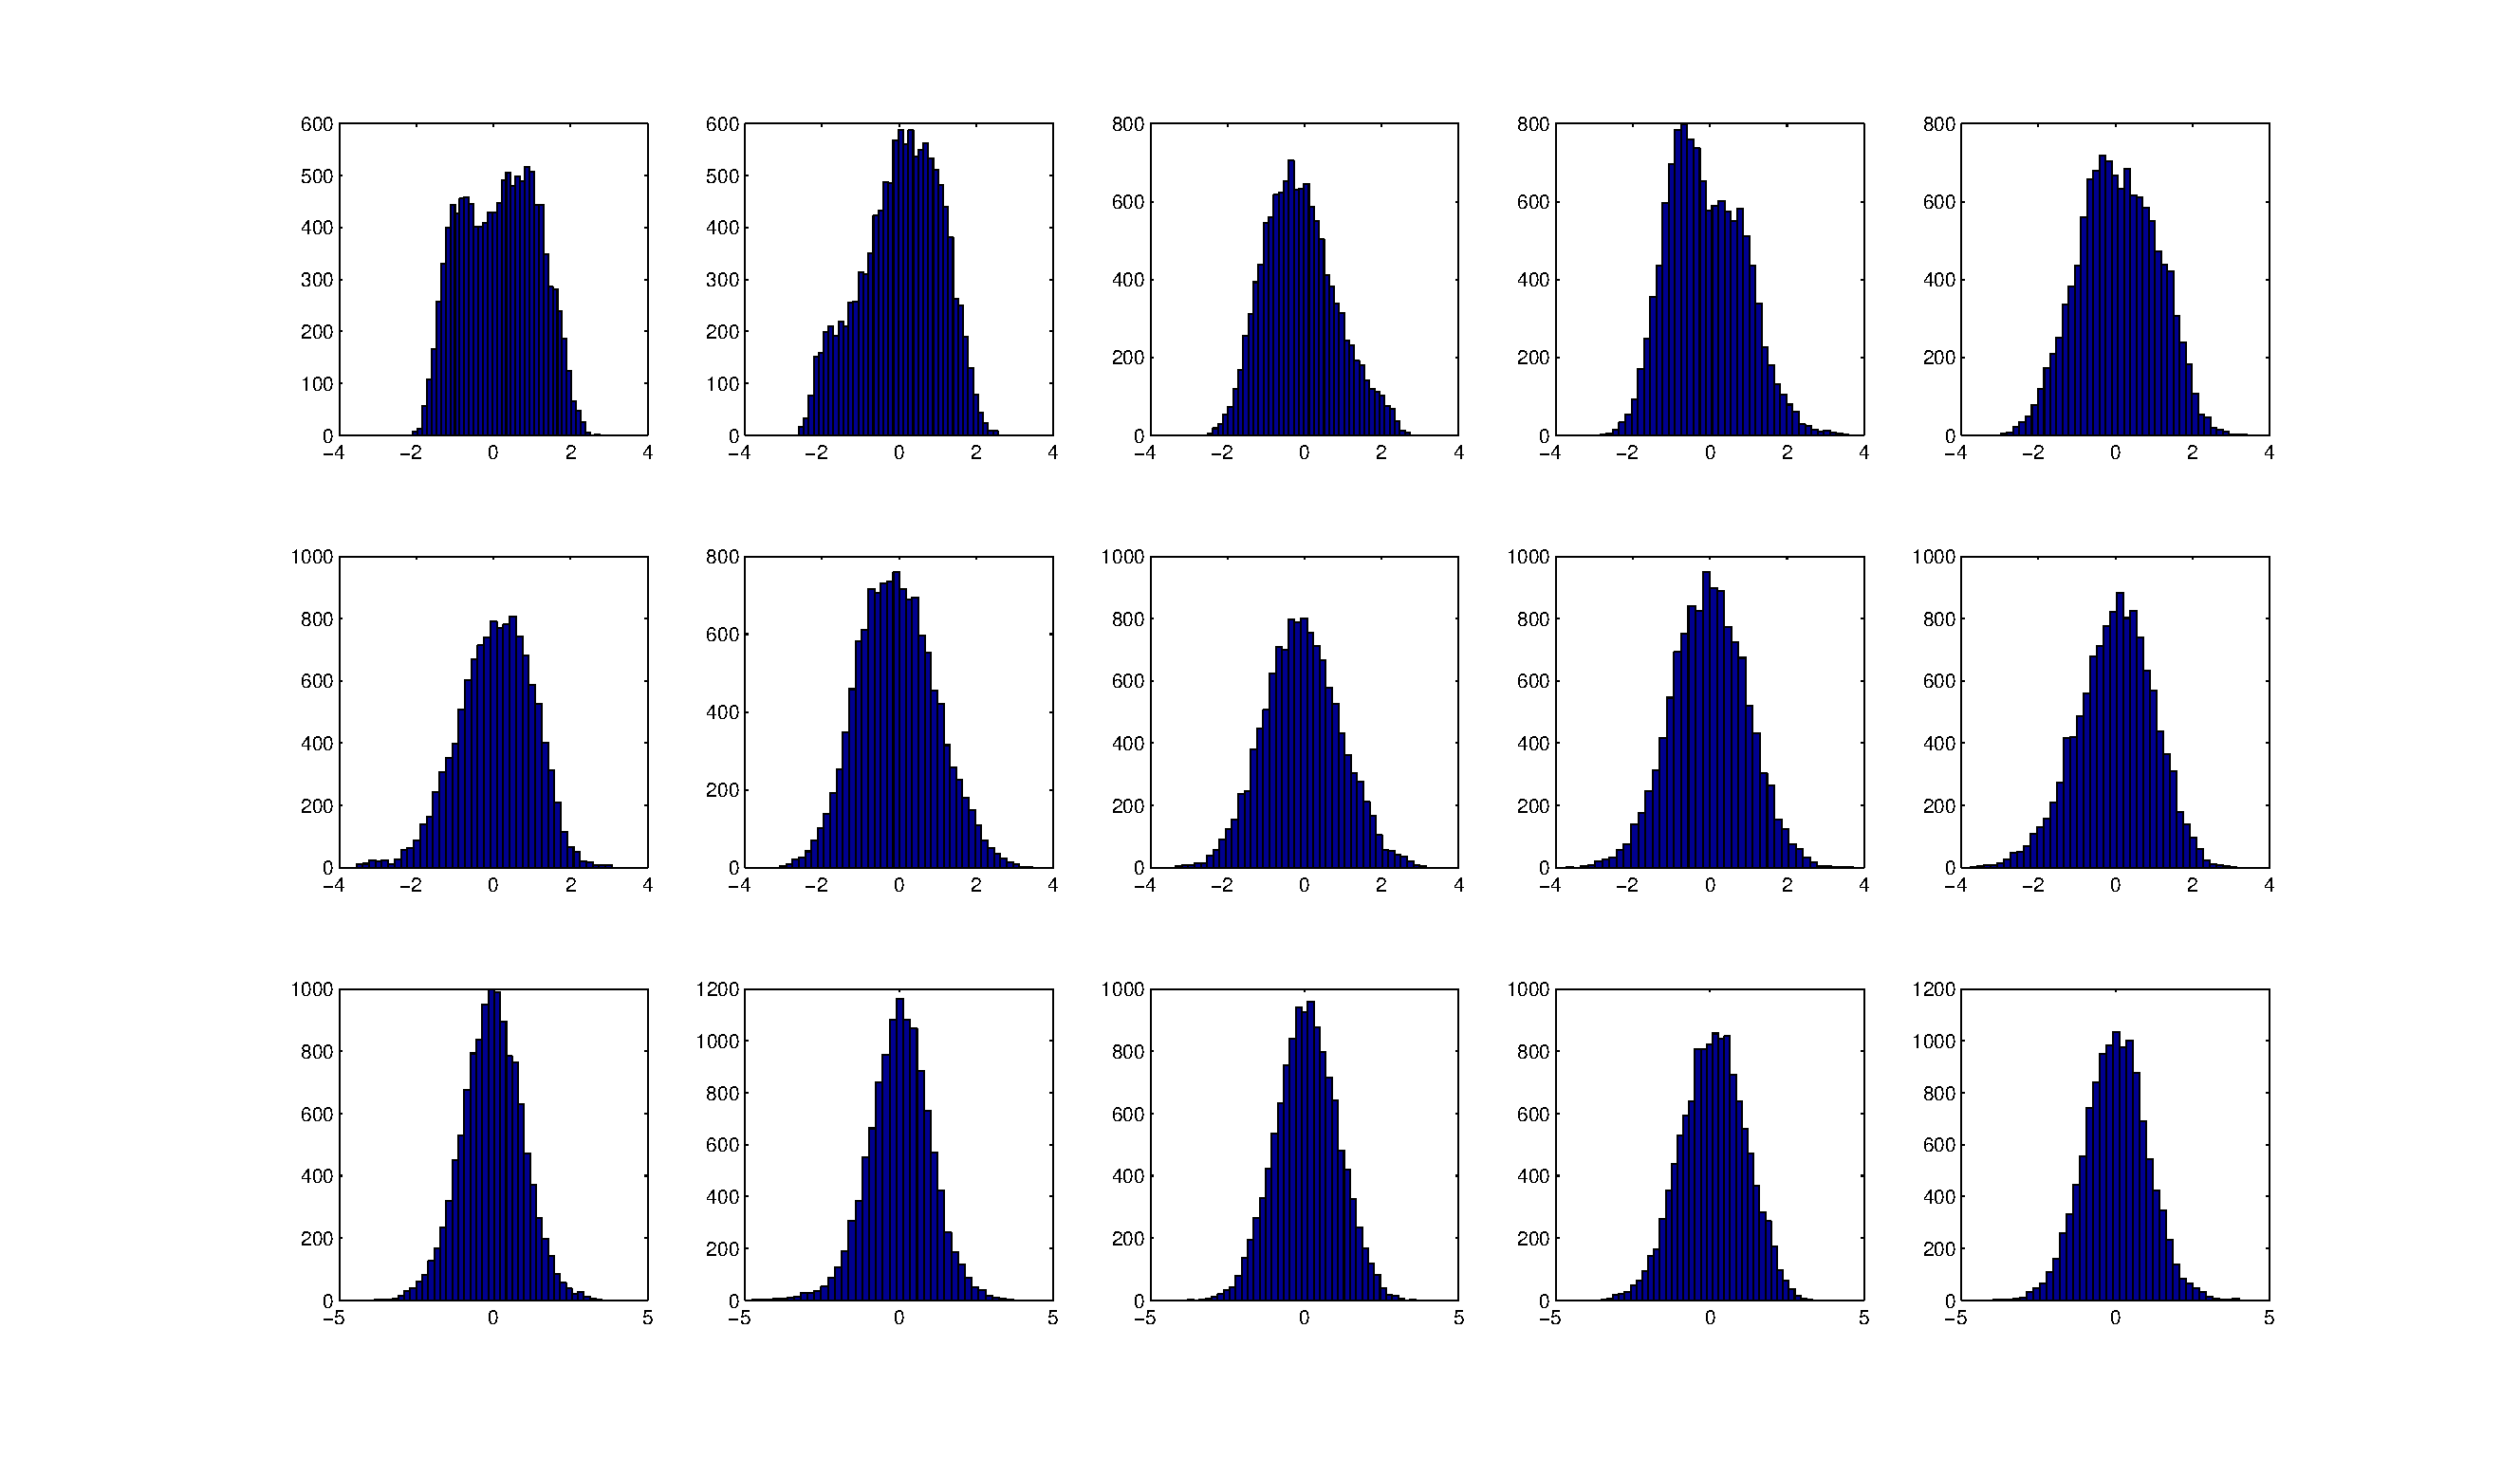
\includegraphics[width=\columnwidth]{figures/hist_pca.eps}
\caption{Histograms of the 15 components of in the feature vectors computed
from apply PCA to the HOG descriptors.}
\label{fig:pca}
\end{figure}

\section{SVM for Encoding Hand Poses}
Similar to Song et al.~\cite{song12}, I attempted to further encode the feature
vectors obtained from PCA into hand pose classes. For each pose
gesture, there is a class for its hand poses, and for all the path
gestures, all of their hand poses are grouped into one class called ``Other''.
Figure~\ref{fig:hand-pose-classes} shows hand pose images from two such classes.

\begin{figure}[tbh]
\centering
\subfigure[Depth-mapped hand pose images from ''POINT'' class.]{
  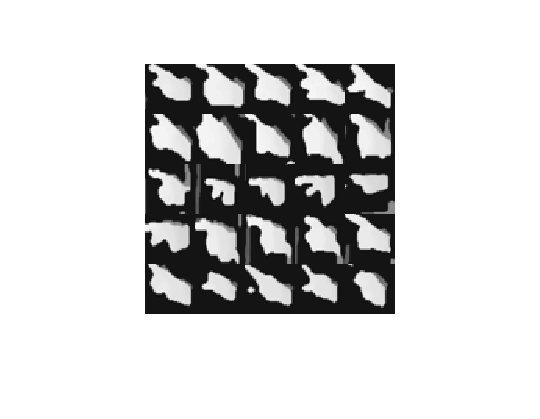
\includegraphics[width=0.5\linewidth,
  trim={0cm 1cm 0cm 0cm}, clip]{figures/point_depth_resize_32_denoise.eps} }
\subfigure[Corresponding HOG descriptor.]{
  \includegraphics[trim={0cm 1cm 0cm 0cm},
  clip, width=0.45\linewidth]{figures/point_depth_hog.eps} }
\subfigure[Depth-mapped hand pose images from ``OTHER'' class.]{
  \includegraphics[width=0.5\linewidth,
  trim={0cm 1cm 0cm 0cm}, clip]{figures/other_depth_resize_32_denoise.eps} }
\subfigure[Corresponding HOG descriptor.]{
  \includegraphics[trim={0cm 1cm 0cm 0cm},
  clip, width=0.45\linewidth]{figures/other_depth_hog.eps} }
\caption{Examples of hand poses from two classes.}
\label{fig:hand-pose-classes}
\end{figure}

I use SVM with
Radial Basis Function (RBF) as the kernel function to do the classification\footnote{
LIBSVM (\url{http://www.csie.ntu.edu.tw/~cjlin/libsvm/}) are used for SVM
related computation.}. Grid search~\cite{hsu10} on the
training data are used to find the misclassification costs and 
$\gamma$ in the RBF kernel function.

It is important to note that the data is highly
unbalanced, for example, there are more instances in the ``Other'' class than
other hand pose classes.
If we ignore the  fact that the data is unbalanced, the resultant classifier
will favor the majority class~\cite{ben2010}. To take this
into account, I assign different misclassification costs, $C_i$, (SVM
soft-margin constants) to each class $i$. If $n_+$ and $n_-$ are the number of
examples in a two -class problem, we choose $C_+$ and $C_-$ such that: 
\begin{align}
\frac{C_+}{C_-} = \frac{n_-}{n_+}
\end{align}
To generalize this to multi-class problems, if $n_1, n_2, \ldots, n_k$ are the
number of examples in a $k$-class problem, we can choose $C_1, C_2, \ldots, C_k$
such as 
\begin{align}
C_1 : C_2 :\ldots : C_k =  \frac{1}{n_1} :  \frac{1}{n_2} : \ldots : 
\frac{1}{n_k}
\end{align}

Using data from one user in the YANG dataset, I compared hand pose
classification results using SVM and my HMM-based gesture recognition algorithm
with mixture of Gaussians (MoG) as the emission probability. There are 5 classes
in total: Point, Palm\_Up, Grab, Rest, and Other. Table~\ref{tab:svm} shows
that using SVM does not give better result.  Figure~\ref{fig:svm-hmm}
shows a visualization of the classification results for a segment in a sequence.
It shows that the HMM-based method has a smoothing effect which helps to improve
performance.

\begin{table}[tbh]
\centering
\begin{tabular}{|l|l|l|l|}
\hline
& \thead{Precision} & \thead{Recall} & \thead{$\mathbf{F_1}$} \\
\hline
SVM & 0.74 & 0.77 & 0.75 \\
\hline
HMM with MoG emission & \textbf{0.81} & \textbf{0.82} & \textbf{0.81} \\
\hline
\end{tabular}
\caption{Comparison of hand pose classification results.}
\label{tab:svm}
\end{table}

\begin{figure}[tbh]
\centering
\includegraphics[width=0.5\textwidth]{figures/svm_hmm.png}
\caption{Visualization of the classification results comparing two methods.
this is a continuous segment in a sequence with two pose gestures: ``Palm up''
and ``Point''.}
\label{fig:svm-hmm}
\end{figure}

SVM can output probabilities instead of hard classifications. It is plausible to
use the probabilities as part of the feature vector. However, unlike the other
features in the feature vector, the probabilities for a particular class from
SVM does not follow Gaussian distribution (see Figure~\ref{fig:svm}). 

\begin{figure}[tbh]
\centering
\includegraphics[width=0.55\textwidth]{figures/hist_svm.eps}
\caption{Histogram of SVM probability output for one class.}
\label{fig:svm}
\end{figure}

As a result, it does not seem to be
effective to add SVM encoding (hard decisions or soft decisions) into the
feature vectors.
%\section{Dictionary Learning}

\section{Discussion}
Based on the above analysis, the final feature vector is a concatenation of
motion features and PCA encoded HOG descriptors. All the features follow
Gaussian or MoG distributions, making it is easy to incorporate them in the
HMM-based models.

The probability output from SVM does not follow Gaussian distribution. This
makes it hard to incorporate them into an HMM-base model which models
compatibility between the output and the hidden state using a conditional probability
distribution (CPD). However, probability output might be useful as part of a
feature vector for a CRF-based model as those models have greater flexibility to
incorporate features (e.g. no CPD required). 

\begin{savequote}
Apparently the child recognizes speech sounds as patterns of gestures.
\qauthor{Israel Rosenfield, \textit{The invention of memory}}
\end{savequote}
\chapter{Unified Gesture Recognition Framework}

As mentioned in the Chapter~\ref{chap:related} Related Work, most prior works
focus on recognizing one form of gestures: either path or pose gestures.
We could conceivably just combine the two forms by first deciding what
category the gesture is and then apply different recognition methods. However making
decisions too early may not be robust. For example, if the system categorizes
the gestures wrongly, it will be hard to correct that in the later stage. We
could also apply two different methods simultaneously, e.g., compute likelihood
from HMMs for path gestures and compute SVM probability scores for pose
gestures, but it is not clear how these probabilities can be compared for making
final decisions.

As a result, I developed a unified probabilistic framework to handle the two
forms of gestures so that probabilities are comparable. During online
recognition, the system makes soft decisions rather than hard decisions, and
propagates probabilities until a response (decision)
from the system is required according to the flow of the currently most likely
gesture.
This chapter gives details about this unified framework.

\section{Gesture Modeling using Hierarchical HMM}
In Section~\ref{sec:temporal-model}, I explained that
a gesture consists of three phases: \textit{pre-stroke}, \textit{nucleus}, and \textit{post-stroke}. 
This temporal model can be represented by a stochastic state
machine (the first level in Figure~\ref{fig:hhmm}).
Each gesture phase includes a sequence of hand/arm movement which can 
also be represented by a stochastic state machine (the second level in the figure), with each state generating an
observation (i.e., the feature vector).
This process can be viewed as a hierarchical HMM (HHMM). We can combine gestures
together to form another stochastic state machine (Figure~\ref{fig:combined}).

\begin{figure}[tbh]
\centering
\includegraphics[clip, width=0.7\columnwidth]{figures/hhmm.pdf}
\caption{State transition diagram of the HHMM representation of gesture phases.
Solid arcs represent horizontal transitions between states; dotted arcs
represent vertical transition, i.e., calling a sub-HMM. Double-ringed states
are end states.}
\label{fig:hhmm}
\end{figure}

\begin{figure}[tbh]
\centering
\includegraphics[width=0.7\columnwidth]{figures/combined.png}
\caption{Stochastic state machine for all gestures. The
hidden states for pre-stroke and post-stroke phases are shared among all the
gestures.
}
\label{fig:combined}
\end{figure}

The HHMM is an extension of the HMM that is designed to model domains with
hierarchical structure and/or dependencies at multiple length/time
scales~\cite{murphy02}. In an HHMM, the states of the stochastic automaton can
emit single observations or strings of observations. Those that emit single
observations are called ``production states'' (blue circles in
Figure~\ref{fig:hhmm}, and those that emit strings are termed ``abstract
state'' (black circles). 

We can represent the HHMM as a dynamic Bayesian network (DBN)~\cite{murphy02} as
shown in Figure~\ref{fig:ahmm}.
The state of the whole HHMM at time $t$ is encoded by the vector $(G_t, P_t, S_t)$ where $G_t$ is the gesture label, $P_t$ is the
phase label, and $S_t$ is the hidden state representing a sub-stage in a
gesture phase. $F_t^d$ is a binary indicator variable that is
``on'' (has value 1) if the lower level HMM at time $t$ has just ``finished''
(i.e., is about to enter an end state), otherwise it is ``off'' (has value 0).
The bottom level $X_t$ are the observations. 

The $F_t^d$ binary indicator in the hierarchical model allows us to do
simultaneous segmentation and recognition. I want to avoid doing segmentation first and then find the most
likely HMM for the given sequence, because segmentation based on
differentiating rest position versus non-rest position will not allow the system
to respond fast enough. I want the system to respond at the beginning of the
post-stroke phase rather then at the beginning of the rest position. In
addition, making a hard decision on segmentation can introduce errors that
are hard to correct later. 

Even though the HHMM gives an appropriate modeling of temporal gestures,
performing exact inference on it can be slow due to the loops in the graphical
model. In the real-time system, I flatten the hierarchical HMM into a one-level
HMM for fast training and inference by creating an HMM state for
every leaf in the HHMM state transition diagram \cite{murphy02}, assuming that
the states in the sub-HMMs are not shared. The effect of The $F_t^d$ binary
indicator can be achieved by modeling the termination probability of each
state, $t(\text{END}|s)$, i.e., the probability for state $s$ to transit to the
end state in the sub-HMM.
This conversion is always done in speech recognition as well for speed and ease of processing.

\tikzstyle{vertex}=[circle, draw, minimum size=16pt, inner sep=0pt]
\tikzstyle{observed-vertex}=[circle, draw, minimum size=16pt, inner sep=0pt,
               fill=black!20] 
\tikzstyle{edge} = [draw, thick, -]
\tikzstyle{directed-edge} = [draw, thick, ->]

\begin{figure}[tbh]
\centering
  \begin{tikzpicture}[auto,swap, scale=2]
    % First we draw the vertices
    \foreach \pos/\name in {{(0, 2)/P_1}, {(1, 2)/P_2}, {(2,2)/P_3},
      {(0, 3)/G_1}, {(1, 3)/G_2}, {(2,3)/G_3},     
      {(0.5,2.5)/F_1^G}, {(1.5,2.5)/F_2^G}, {(2.5, 2.5)/F_3^G},
      {(0.5,1.5)/F_1^P}, {(1.5,1.5)/F_2^P}, {(2.5, 1.5)/F_3^P}, {(0, 1)/S_1},
      {(1, 1)/S_2}, {(2, 1)/S_3}} 
      \node[vertex] (\name) at \pos {$\name$};
    \foreach \pos/\name in {{(0, 0.5)/X_1}, {(1, 0.5)/X_2}, {(2, 0.5)/X_3}}
      \node[observed-vertex] (\name) at \pos {$\name$};
    % Connect vertices with edges and draw weights
    \foreach \source/ \dest in {P_1/S_1, S_1/X_1, P_1/F_1^P, S_1/F_1^P,
        G_1/P_1, G_2/P_2, G_3/P_3, G_1/G_2, G_2/G_3,
        G_1/F_1^G, G_2/F_2^G, G_3/F_3^G, P_1/F_1^G, P_2/F_2^G, P_3/F_3^G,
        F_1^G/G_2,  F_2^G/G_3, F_1^G/P_2, F_2^G/P_3, 
        F_1^P/F_1^G, F_2^P/F_2^G, F_3^P/F_3^G, 
        F_1^P/P_2, P_1/P_2, P_2/S_2, S_2/X_2, P_2/F_2^P,
        S_2/F_2^P, F_2^P/P_3, P_2/P_3, P_3/S_3, S_3/X_3,
        P_3/F_3^P, S_3/F_3^P, S_1/S_2, S_2/S_3,
        F_1^P/S_2, F_2^P/S_3} 
      \path[directed-edge] (\source) -- (\dest);
  \end{tikzpicture}
  \caption{DBN representation of the HHMM for the temporal gesture model. $G_t$ is the gesture label, $P_t$ is the
phase label, and $S_t$ is the hidden state representing a sub-stage in a
gesture phase. $F_t^d = 1$ if the HMM at the lower level has finished
(entered its exit state), otherwise $F_t^d = 0$. Shaded nodes are observed; the
remaining nodes are hidden.}
  \label{fig:ahmm}
\end{figure}

\section{Unified Framework}
I flatten the HHMM into a single level HMM with discrete hidden states 
representing sub-stages of gesture phases. The assumption is that
gesture phases of different gestures do not share sub-stage hidden states.

Based on the standard HMM\footnote{See Appendix~\ref{app:hmm} for more details
about HMM.} formulation, the probability of a sequence of observation, $\underline{x}_{1:T} = \underline{x}_1\ldots\underline{x}_T$, and
the corresponding hidden states sequence, $s_{1:T} = s_1\ldots s_T$, is given by
\begin{align}
P(\underline{x}_{1:T}, s_{1:T};\underline{\theta}) = 
    t(s_1)t(\text{END}|s_T)\prod_{t = 2}^T t(s_t | s_{t-1})\prod_{t = 1}^T
    e(\underline{x}_t|s_t)\label{eq:hmm}
\end{align}
where $\underline{\theta}$ represents the model parameter vector which includes
the initial state probabilities $t(s)$, the state transition probabilities $t(s'|s)$, the 
emission probabilities $e(\underline{x}|s)$,
and the termination probabilities $t(\text{END}|s)$ for $s, s'\in \{1, 2,\ldots
k\}$. In this section, I describe how I model these conditional
probability distributions (CPDs), and compute the model parameters for both
path and pose gestures, combining them together under the unified HMM-based
framework. Note that the term ``unified framework'' means that the two forms of
gestures are combined under the same probabilistic framework, but there are
still differences in the models for the two gestures, e.g., different topologies
and different training strategies.

\subsection{Path Gestures}
If we have ground truth labels for the pre-stroke, the nucleus and the
post-stroke phases as in the ChAirGest dataset, we can train the sub-HMMs for
each phase and each gesture separately and then concatenate them (i.e., the
concatenated HMMs\footnote{See my previous publication~\cite{yin13} for
details.}).
However in practice, for example if we want users to be able to easily add their new gestures by giving a few
examples, it will be tedious to manually label the start and the end of the
three phases. In this case, I use embedded training \cite{young1994}, i.e.
train each phase sub-HMM embedded in an entire gesture segment
(Figure~\ref{fig:embed}).

\begin{figure}[tbh]
\centering
\includegraphics[width=0.7\columnwidth]{figures/embedded.pdf}
\caption{Embedding phase HMMs into an entire gesture.}
\label{fig:embed}
\end{figure}

With the YANG dataset, I choose to use one hidden state for pre-stroke and
post-stroke phases through cross-validation. I use the Bakis (left-right with
skips) topology~\cite{Bauer00} for the nucleus phase, but add a backward
transition from the last hidden state to the first one for gestures with an arbitrary number of repetitions (e.g., ``Wave''
gesture) (Figure~\ref{fig:bakis}). The left-right topology not only closely
models the temporal evolution of a gesture, it also reduces the model complexity
by constraining the number of possible transitions. Without this constraint,
the model would have $O(K^2)$ transition parameters; with the left-right
constraint, the model only has $O(K)$ transition parameters where $K$ is the
number of hidden states in the HMM.

\tikzstyle{vertex}=[circle, draw, minimum size=16pt, inner sep=0pt]
\tikzstyle{observed-vertex}=[circle, draw, minimum size=16pt, inner
sep=0pt, fill=black!20] 
\tikzstyle{edge} = [draw, thick, -]
\tikzstyle{directed-edge} = [draw, ->]
\begin{figure}[tbh]
\centering
  \begin{tikzpicture}[auto,swap, scale=1.5]
    % First we draw the vertices
    \foreach \pos/\name in {{(0, 0)/start}, {(1, 0)/s_1}, {(2, 0)/s_2},
    {(3, 0)/s_3}, {(4, 0)/s_4}, {(5, 0)/end}}
      \node[vertex] (\name) at \pos {$\name$};
    % Connect vertices with edges and draw weights
    \foreach \source/ \dest in {s_2/s_3, s_3/s_4, s_4/end,
    s_1/s_2} \path[directed-edge] (\source) -- (\dest);
    
    \foreach \source/ \dest in {s_1/s_3, start/s_2, s_2/s_4, s_3/end, s_4/s_1} 
      \path[directed-edge] (\source) edge [bend left] (\dest);
      
    \foreach \source/ \dest in {s_1/s_1, s_2/s_2, s_3/s_3, s_4/s_4} 
      \path[directed-edge] (\source) edge [loop above] (\dest);
    
    \path[directed-edge] (start) edge node [below] {$t(s_1)$} (s_1);
  \end{tikzpicture}
  \caption{A state transition diagram of a modified 4-state Bakis model for the nucleus phase.}
  \label{fig:bakis}
\end{figure}

In Chapter~\ref{chap:feature}, I showed that the features I use follow mixture
of Gaussians (MoG) distributions, hence I use MoG with diagonal covariances to
model the emission probability, i.e.,
\begin{align}
e(\underline{x} | s) = \sum_{m=1}^k q(m | s)\mathcal{N}(\underline{x};
\mu_{s,m}, \Sigma_{s, m})
\end{align}
where $k$ is the number of mixtures.
Figure~\ref{fig:mog} shows the DBN representation of an HMM of MoG emission
probabilities. The covariance, $\Sigma_{s, m}$, has a fixed prior of $0.01\times
I$ which is added to the maximum likelihood estimate to prevent the covariance from shrinking to a point/delta function. 

\begin{figure}[tbh]
\centering
\includegraphics[width=0.5\columnwidth]{figures/mog.png}
\caption{DBN representation of HMM with mixture of
Gaussians emission probabilities.}
\label{fig:mog}
\end{figure}

\subsubsection{Training Strategies}
I use a two-pass training to estimate the model parameters for each path
gesture HMM separately. Currently, training is done in MATLAB using Kevin
Murphy's HMM toolbox\footnote{\url{https://code.google.com/p/bnt/}}.

The first pass is Viterbi training\footnote{See Appendix~\ref{sec:viterbi} for
details}.
In this pass, only the first state (i.e., the pre-stroke hidden state) can be the initial state and the last state
(i.e., the post-stroke hidden state) can be the termination state. The emission
probability parameters are initialized by uniformly segmenting the data and
associating each successive segment with successive states~\cite{young1994}. For
each segment, the K-means algorithm is used to initialize MoG parameters. In
each iteration of the training, the most likely path is computed using the
Viterbi algorithm. For all the observations assigned to the same hidden
state, K-means algorithm is used again to find the new MoG parameters for
that state. The Viterbi training provides a better alignment of data with the
hidden states, and thus gives a better initialization of the MoG parameters. 

The second pass is Baum-Welch training that computes the maximum likelihood
estimate of the parameters.
It uses the estimated MoG parameters as the initial values. It also relaxes the
initial state probabilities (allowing the first two states to be the start
state) and the termination probabilities (allowing the last two states to be the
termination state). This allows the possibility of transitions between nucleus
phases without going through pre-strokes and post-strokes when we combine the
individual gesture HMMs together. For natural interaction, this is important
because sometimes users may do a gesture immediately after another. When
initializing the transition matrix, all the allowed transitions are set to the same value, so that no states are favored arbitrarily. Transitions that are not allowed are initialized to zero.

The Baum-Welch estimation formulae for MoG parameters and transition parameters
are well established. Here, I give the formula for the termination probability.
Given $N$ training sequences, the update for the termination probability during the $i$th iteration is 
\begin{displaymath}
t^i(\text{END}|s) = \frac{\sum_{j = 1}^N \overline{count}(j, s\rightarrow
END;\underline{\theta}^{i-1})} {\sum_{j = 1}^N\sum_{s'} \overline{count}(j, s\rightarrow s';\underline{\theta}^{i-1})}
\end{displaymath}
where $\overline{count}(j, s\rightarrow END;\underline{\theta}^{i-1})$ is the expected count of 
$s$ being the end state. We can use the usual forward-backward algorithm to compute all the 
expected sufficient statistics by adding a dummy END state to the end of each
sequence (see Appendix~\ref{sec:term} for details).

\subsection{Pose Gestures}
I use one hidden state to represent pose gestures. Let
$s_{\text{pose}}$ be the single hidden state for the nucleus phase of a
pose gesture (Figure~\ref{fig:single}). Within a user,
there may be variation in the hand pose for a gesture with distinct hand pose.
For example, the Point hand pose can have different orientations.
Hence, I also use the MoG for the emission probability
$e(\underline{x} | s_\text{pose})$. 

\begin{figure}[tbh]
\centering
\includegraphics[width=0.5\columnwidth]{figures/single_state.pdf}
\caption{State transition diagram of a single state HMM for gestures with
distinct hand poses. }
\label{fig:single}
\end{figure}

The number of mixtures for pose gestures are greater than that of path
gestures however, and they can be different for different pose gestures. This is
because some hand poses may have more variation than others.
For example, the Point gesture may have more variations in orientations than
Grab gesture (hand in fist).

\subsubsection{Training Strategies}\label{sec:pose-gesture}
Instead of doing embedded
training, I directly compute the maximum likelihood estimates of the MoG
parameters for emission probability of $s_{\text{pose}}$ because there is only
on hidden state.

The number of mixtures is
determined using Bayesian Information Criterion (BIC)~\cite{fraley06}:
\begin{align*}
\text{BIC}\eqdef2\text{loglik}(\underline{x}_{1:n}, \underline{\theta}_k^*) -
(\text{\# params})\log(n)
\end{align*}
where $\text{loglik}(\underline{x}_{1:n}, \underline{\theta}_k^*)$ is the
maximized loglikelihood for the data and the model with $k$ mixtures per state, (\# params) is the number of independent parameters to be estimated in the model, and $n$ is the number of observations in
the data. Let $d$ be the feature vector dimension, then $\mu_{s,m}$ for
hidden state $s$ and mixture $m$ has $d$ independent parameters, and the
diagonal covariance matrix $\Sigma_{s,m}$ has $d$ independent parameters as
well. Because $\sum_{m=1}^k q(m | s) = 1$, the number of independent parameters
for the weights $q(m|s)$ is $k - 1$. Hence,(\# params) is computed as:
\begin{align*}
\text{\# params} = (k - 1) + (d + d) * k
\end{align*}
The $k$ that gives the highest BIC is chosen from a predetermined range.

For each $k$, Expectation Maximization (EM) is used to estimate the means,
covariance matrices and mixture probabilities of the MoG. As the EM algorithm may
converge to a local optimum of the observed data likelihood~\cite{dicintio12}, I
repeat the optimization 3 times using K-means algorithm with random
initialization to set the initial cluster centers, and choose the model that
gives the maximum likelihood.

The training data for pose gestures should contain random variations in the
hand movement so that the resultant variances for the motion features will be
larger, making motion features less important in
$e(\underline{x}|s_{\text{pose}})$. In Figure~\ref{fig:covariance}, I compare
two covariance matrices of MoG for hidden states from two forms of gestures. The
variance values are normalized between the two matrices for each feature to make
them comparable. We can see that the variances for the motion features (features
1--9) are larger for the pose gesture.

\begin{figure}[tbh]
\centering
\subfigure[Hidden state of a path gesture.]{
\includegraphics[trim=1.3cm 0 1cm
0.5cm, clip, width=0.45\columnwidth]{figures/covariance_path.eps} }
\subfigure[hidden state of a pose gesture.]{
\includegraphics[trim=1.3cm 0
1cm 0.5cm, clip, width=0.45\columnwidth]{figures/covariance_pose.eps} }
\caption{Visualization of normalized covariance matrices of MoG for different
hidden states. The darker the color, the larger the variance.}
\label{fig:covariance}
\end{figure}

It is possible that a gesture with a distinct path also has the same hand pose
as another gesture with distinct hand pose, for instance, some user may prefer
to do the Circle gesture with a point hand pose. In this case, the gesture
will be recognized as the Circle gesture because it matches both the hand
pose and the path and thus the Circle gesture would have a higher likelihood
after considering a few consecutive frames.

Since there is only one hidden state for $s_{\text{pose}}$, its transition
probability is 1. Its termination probability is estimated according to the
expected duration of the gesture. The self-arc on a state in an HMM defines a 
geometric distribution over waiting time \cite{murphy02}. In the case of a
single state HMM, the probability of remaining in state $s_{\text{pose}}$ for
exactly $d$ steps is $P(d) = p(1-p)^{d - 1}$, where $p = P(END|s_\text{pose})$
is the termination probability for $s_{\text{pose}}$. This means the expected
number of steps remaining in state $s_{\text{pose}}$ is $\frac{1}{p}$. I assume
that the minimum duration of a path gesture is one
second (30 frames). The termination probability $P(END|s_\text{pose})$ is then set to
be less than $\frac{1}{30}$.

I also use one hidden state to model the rest position in a similar way.

\section{Real-time Gesture Recognition}
I train one HMM, $\underline{\theta}_g$, for each gesture (path or pose) $g\in
\{1\ldots G\}$, then combine them into a one-level flattened HMM, assuming uniform transition probabilities among gestures.

\subsection{Combined HMM}
I use the superscript $c$ to denote the model
parameters in the combined HMM. Let $K_{g}$ be the number of hidden states for
gesture $g$. The total number of hidden states in the combined HMM, $K^c$, is then
\begin{align*}
K^c = \sum_g K_{g}
\end{align*}
The model for each path gesture starts with a hidden state for the pre-stroke,
then 1 or 2 hidden states for the nucleus, followed by a hidden state for the
post-stroke. Each pose gesture has a hidden state for the nucleus. The combined
HMM has a sequential labeling for these models' hidden states, with the hidden state label for the pre-stroke of the second gesture model following
the hidden state label for the post-stroke of the previous gesture, etc.
Formally, the new hidden states labels are in $\{1\ldots K^c\}$, and
the hidden states from $(\text{base}_i + 1)$ to $(\text{base}_g + K_{g})$
belongs to gesture $g$ where $base_g$ is the base index
\begin{align*}
\text{base}_g = \sum_{j=1}^{g-1}K_{j}
\end{align*}
Figure~\ref{fig:combined-hmm} gives an example of the labeling scheme in
the combined HMM. This scheme allows me to easily map a hidden state label back
to its corresponding gesture and phase.

\begin{figure}[tbh]
\centering
\includegraphics[width=0.9\columnwidth]{figures/combined_hmm.png}
\caption{Combined HMM. The red lines are examples of new transitions. Not all
possible transitions are shown to avoid cluttering the diagram.}
\label{fig:combined-hmm}
\end{figure}

The non-trivial part in creating the combined HMM is computing the new 
transition probabilities. The initial state probability in the combined
HMM, $t^c(s)$, for $s\in\{1\ldots K^c\}$ is
\begin{align*}
t^c(s) = \frac{t(s)}{\sum_{s'=1}^{K^c} t(s')}
\end{align*}
The probability of an $s$ to $s'$ transition
in the combined model is the sum over all paths from $s$ to
$s'$ for $s, s'\in\{1\ldots K^c\}$~\cite{murphy02}. In our model, 
\begin{align}
t^c(s'|s) = t(s' | s) (1-t(\text{END}|s)) +
t(\text{END}|s)t^c(s')
\label{eq:combined-transition}
\end{align}
where $t(s'|s)$ is the transition probability in the individual gesture HMM if
$s$ and $s'$ are from the same gesture; otherwise it is zero. Note that
$t(s'|s)$ is normalized such that $\sum_{s'}t(s'|s) = 1$ without taking into
account the termination probability $t(\text{END}|s)$ (as the end state is not
an actual hidden state), hence it is necessary to multiply $t(s'|s)$ by $
(1-t(\text{END}|s))$ in Equation~\ref{eq:combined-transition} to get the actual
unnormalized probability.

As the pre-strokes and post-strokes for different gestures can be similar, I
allow sharing of the pre-strokes and post-strokes by adding a small probability
(0.01) among pre-stroke hidden states and among post-stroke hidden states.

Finally, we need to make sure that the new transition matrix is stochastic,
i.e., 
\begin{align*}
\sum_{s' = 1}^{K^c} t^c(s'|s) = 1
\end{align*}
by normalizing $t^c(s'|s)$.

\subsection{Online Inference}
Once we have a combined model, I use fixed-lag smoothing \cite{murphy02} to do
online inference on the flattened HMM for real-time gesture recognition.
Fixed-lag smoothing is a modified forward-backward algorithm. Unlike online
filtering, which estimates the belief state at current time $t$ using forward
pass only, we estimate the state at $t - l$, given all the evidence up to the
current time $t$, i.e., compute $\gamma_{t - l}(s) \eqdef P(S_{t -
l} = s|\underline{x}_{1:t})$, where $l > 0$ is the lag (see
Figure~\ref{fig:inference}).
Introducing lag time is a tradeoff between accuracy and responsiveness. Using some future evidence to
smooth the estimate can increase the accuracy while adding some delay. However
if the delay is small, it might be unnoticeable.
In the Experiment Evaluation section (Section~\ref{sec:evaluation}), we show
details about the relationship between $l$ and the recognition performance.

\begin{figure}[tbh]
\centering
\includegraphics[width=0.5\columnwidth]{figures/inference.png}
\caption{Figure adapted from~\cite{murphy02} comparing different kinds of
inference. The shaded region is the interval for which we have data. The arrow
represents the time step at which we want to perform inference. $t$ is the
current time, and $T$ is the sequence length (see Appendix~\ref{sec:inference}
for details).}
\label{fig:inference}
\end{figure}

Fixed-lag smoothing can be implemented efficiently. We compute forward
probabilities $\alpha_t(s) \eqdef P(S_t = s|\underline{x}_{1:t})$
normally\footnote{It is more common (see e.g.,~\cite{Rabiner90}) to define
$\alpha_t(s) = P(S_t = s, \underline{x}_{1:t})$; the difference is discussed in
Appendix~\ref{sec:hmm-infernece}.} and keep a history window of
$\alpha_{t - l}\ldots\alpha_t$.
At every time frame, we compute backward probabilities $\beta_{t-l}(s)\eqdef
P(\underline{x}_{t-l+1:t}|S_{t-l}=s)$ from current time $t$ to $t - l$, i.e.,
form $l=0$ to $l$.
Then we can compute
\begin{align}
\gamma_{t - l} \eqdef P(S_{t-l}=s|\underline{x}_{1:t-l}) \propto \alpha_{t -
l}
\cdot
\beta_{t - l}
\end{align}  
The time complexity at each time frame is $O((K^c)^2l)$. Note that at time $t$,
the belief state at $t - l$ is committed, while the belief state from $t - l + 1$ to $t$
will still be revised later.

We can then compute the most likely hidden state at $t - l$:
\begin{align}
\hat{s} = \arg\max_s \gamma_{t - l}(s)
\end{align}
The most likely hidden state is then mapped to the gesture label it
belongs to (including the rest position) and the gesture phase. 

Gesture events are detected at the boundary of a phase change: start pre-stroke,
start gesture nucleus and start post-stroke. In this way
we achieve simultaneous segmentation and recognition. The gesture event
information, together with the gesture label for the nucleus phase, are sent to the application level.
The system achieves real-time performance at 30FPS.

\begin{figure}[t]
\centering
\includegraphics[trim=0 5mm 0
5mm, clip, width=\columnwidth]{figures/hidden_labeled.jpg}
\caption{Most likely hidden states using fixed-lag smoothing. Different colors indicate different hidden states. Yellow indicates rest position.}
\label{fig:visual_hidden}
\end{figure}

Figure~\ref{fig:visual_hidden} shows a visualization of the
most likely hidden states based on online fixed-lag smoothing inference
with $l = 5$ on a test sequence from the YANG dataset.
This is based on an input sequence of 6 gestures. The first 3 gestures are
Circle and the last 3 gestures are Horizontal Wave gestures. Notice that in
the first segment, at the beginning, the most likely hidden state is the
pre-stroke for Horizontal Wave, but since a response is not required at this
time, the wrong estimate does not matter. After a few more frames, the estimates are
updated to have the correct most likely gesture label and the system
responds correctly when it detects the start of the post-stroke of Circle
gesture.

\section{Gesture Spotting}
Identifying gesture phases allows us to distinguish gestures from non-gestures.
As every gesture must have a nucleus, any hand movement that does not have a
nucleus phase can be identified as non-gesture. 

For example, when performing offline recognition on the ChAirGest dataset, I use
MoG models for rest and non-rest positions to find non-rest segments (i.e.,
segments with hand movement) in a test sequence, and for a non-rest segment, use
the Viterbi algorithm to find the most probable hidden state sequence $\hat{s}_1\ldots\hat{s}_T$ using
the mostly likely gesture model $\underline{\theta}_{\hat{g}}$
(see~\cite{yin13} for details).
Again, each hidden state can by classified into a pre-stroke
($s_\text{pre-stroke}$), nucleus ($s_\text{nucleus}$), or post-stroke
($s_\text{post-stroke}$) state.
The start and the end time for a gesture nucleus are the first and the last time
frame $t$ where $\hat{s}_t\in s_{\text{nucleus}}$ respectively. 

\begin{figure}[!tbh]
\centering
\subfigure[Gesture label result.
The pre-stroke and post-stroke phases are indicated by two orange colors (see the color bar).]{
\includegraphics[trim={4cm 1cm 0cm 0.6cm}, clip,
width=1\columnwidth]{figures/gesture.eps}\label{fig:gesture-label}
}
\subfigure[Most probable hidden states.
Colors 1-3 indicate the pre-stroke hidden states, colors 4 - 9
indicate the nucleus hidden states, colors 10 - 12 indicate the post-stroke
hidden states, and color 14 indicates the rest state.]{
\includegraphics[trim={2.5cm 0cm 0.2cm 0cm}, clip,
width=1\columnwidth]{figures/hiddenstates_labeled.jpg} \label{fig:hiddenstates}
}
\caption{Visualization of gesture recognition result. A non-rest segment
without a nucleus phase (see $t\sim 30700$ in \subref{fig:hiddenstates}) is not
identified as a gesture (no label reported at the same time in
\subref{fig:gesture-label}.}
\end{figure}

Figure~\ref{fig:gesture-label} shows the recognition result visualization for
one test sequence. The first row is the ground truth with different colors
indicating different gesture phases or the rest position.
The second row is my segmentation and recognition result.
Figure~\ref{fig:hiddenstates} shows the color-coded most probable hidden states
for the same sequence.
If a non-rest segment does not contain hidden states belonging to the nucleus
phase, it is ignored (see the blue bar at $t\sim 30700$ in Figure~\ref{fig:hiddenstates}).
In this way, we can spot the actual gestures while filtering out other movements.

Using a thresholding method on the loglikelihood of a
given segment may not be robust because the maximum loglikelihood of a non-gesture
segment among all gesture HMMs can be greater than that of a gesture segment.
The HMM formulation (Equation~\ref{eq:hmm}) implies that the longer the sequence the smaller the
likelihood (and hence the loglikelihood) because there are more probability
terms which are all smaller than 1 in the product terms. For example, the
loglikelihood of the fifth non-rest segment (a non-gesture) in
Figure~\ref{fig:hiddenstates} has a maximum loglikelihood of -296.6, while the
first non-rest segment (a gesture) has a maximum loglikelihood of -785.6. 
Even if we normalize the loglikelihoods by the segment lengths, the normalized
loglikelihood for the non-gesture (-14.8) is still greater than that of the
gesture (-17.9). As non-gestures are often shorter than gesture sequences, it
would hard to set a good threshold.
 
My gesture phase based method can be used in addition to a thresholding method
with a relative conservative threshold, i.e., a threshold that may cause false
positives but no false negatives so that the gesture phase based method can be used to further
filter out false positives.

\section{Concatenated HMM versus LDCRF}
Morency et al. formulated LDCRF~\cite{morency07} (an extension to CRF), and used
it for head and eye gesture recognition. In contrast to HMM which is a
generative model, LDCRF is a discriminative model. It gives
per frame classification, and hence, can 
be used to do simultaneous segmentation and labeling as well. I applied LDCRF to gesture phase segmentation and recognition, and
compared the result with my concatenated HMM method~\cite{yin13}. 

As LDCRF requires per frame labeled training data, we need ground truth labeling
for the gesture phases. Hence, I use the ChAirGest dataset for this
evaluation. For all the non-rest segments in the training set, the nucleus
frames are labeled $1\sim 10$ according to their corresponding gesture labels.
All the pre-stroke frames are labeled 11, and all the post-stroke
frames are labeled 12. This means the pre-strokes of all the gestures share the
same hidden states, and same for post-strokes. Using different hidden states
for pre-strokes and post-strokes of different gestures would increase
computation time significantly since it increases quadratically with the number
of hidden states (see Appendix~\ref{sec:linear-crf}). For each label, 6 hidden
states are used, resulting in 72 hidden states in total.

During testing, frames from the non-rest segments are classified into gesture
nucleus labels, pre-stroke or post-stroke using the trained LDCRF model. Using
the pre-stroke and post-stroke labels, we can find the start and end of the
nucleus phases. The HCRF
library\footnote{\url{http://sourceforge.net/projects/hcrf/}} which contains an implementation of the LDCRF model is used for both training and testing.

Table~\ref{tab:ldcrf} shows a comparison of the results between
using LDCRF and concatenated HMMs. The $F_1$ score of the concatenated HMMs
model is 7.7\% higher (absolute difference) than the LDCRF model. However,
the LDCRF gives slightly higher (1.5\%) temporal segmentation score, ATSR.
Overall, the concatenated HMMs gives better performance (6.0\% higher) and takes
orders of magnitude less time to train.

\begin{table}[tbh]
\centering
\begin{tabular}{|l|l|l|}
\hline
& \thead{LDCRF} & \thead{Concatenated HMMs} \\
\hline
$F_1$ Score & 0.82 (0.03) & \textbf{0.897 (0.03)} \\
\hline
ATSR Score & \textbf{0.923 (0.02)} & 0.907 (0.02) \\
\hline
Final Score & 0.84 (0.02) & \textbf{0.90 (0.02)} \\
\hline
Training Time & 18hr & \textbf{7min} \\
\hline
\end{tabular}
\caption{Comparison of recognition results between LDCRF and concatenated
HMMs using the ChAirGest dataset.}
\label{tab:ldcrf}
\end{table}

\subsection{LDCRF Optimization}
One reason that LDCRF is so slow is that it considers all pair-wise transitions
among all the hidden states in the optimization process ($72^2$ transition
features in this case). However, since the hidden states are not shared among
gestures, we do not need to consider the transitions between hidden states
from different gestures. In order to decrease the training time, I reduce the
time complexity of the model by constraining allowed transitions among hidden states.

In HMM, we can specify the topology by initializing transitions that are not
allowed to zero. In LDCRF, I do the same by setting transitions that are not
allowed to always be zero (or negative infinity if loglikelihood is used) in
each update. The edge features only include allowed transitions as well,
reducing the number of features in the model needs to optimized. A 
mask matrix is used to specify allowed transitions, can I call this masked
LDCRF. Using this optimization, I am able to reduce the training time to 11hr.


\chapter{Hybrid Performance Metrics}
It is important to have metrics that can accurately evaluate and compare
performances of different algorithms for a given task domain. We should
be aware that a metric that is good for one task, is not
necessarily appropriate for another task. 

\section{Existing Methods for Error Scoring}
Gesture recognition can be considered as a sub-domain of human activity
recognition. Two basic units of comparison are typically used in this field
-- frames or events:

\textit{Scoring Frames.} A \textit{frame} is a fixed-length,
fixed-rate unit of time. It is often the smallest unit of measure defined by the system \cite{ward11}, and in such cases approximates continuous time.
For example, in our case, a frame is a data frame consisting of a RGB data frame, a depth data frame and a skeleton data from the
sensor at 30 FPS. Because of the one-to-one mapping between ground truth and
output, scoring frames is trivial, with frames assigned to one of: true positive
(TP), true negative (TN), false positive (FP) or false negative (FN). Commonly
recommended frame-based metrics include: true positive rate (TPR $= \frac{TP}{TP
+ FN}$), false positive rate (FPR $= \frac{FP}{TN + FP}$), precision
($\frac{TP}{TP + FP}$).

\textit{Scoring Events.} An \textit{event} is a variable duration sequence of
frames within a continuous time-series.  It has a start time and a stop time.
Given a test sequence of $g$ known events, $E = [e_1, e_2, \ldots, e_g]$, a
recognition outputs $h$ return events, $R = [r_1, r_2, \ldots, r_h]$. There is
not necessarily a one-to-one relation between $E$ and $R$. A comparison can
instead be made using alternative means such as dynamic time warping
(DTW)~\cite{berndt94} or edit distances~\cite{guyon13}. An event can then be
scored as either correctly detected (C), falsely inserted (I), or deleted
(D)~\cite{ward11}. Event scores can be summarized
by precision ($\frac{C}{h}$), and recall
($\frac{C}{g}$).

\section{Shortcomings of Conventional Performance Characterization}
Either frame-based or event-based metrics 
alone may not be adequate for evaluating a real-time continuous gesture recognition system handling different types of gestures. We illustrate this using examples from related works.

Both ChaLearn Gesture Challenge 2012~\cite{guyon13} and Multimodal Gesture
Recognition Challenge 2013~\cite{escalera2013} use the Levenshtein edit
distance\footnote{\url{http://en.wikipedia.org/wiki/Levenshtein_distance}},
$L(R, E)$, between the ordered list of recognized events ($R$) and the ground
truth events ($E$) to evaluate performance. However, such event-based metrics
that ignore the timing offset errors are inadequate to identify true positives
in sequences. For example, in Figure~\ref{fig:edit-distance}, both Algorithm 1
and Algorithm 2 would have the same score using their metric. However, Algorithm
1 is in fact worse because the recognized event B is mistakenly considered as a
true positive in the minimum edit distance calculation, and the number
of mistakes should be 3.
Consider a real-time application, if the user does gesture A, it cannot be considered correct if the
system responds to gesture B.

\begin{figure}[tbh]
\centering
\includegraphics[width=0.8\textwidth]{figures/edit_distance.png}
\caption{Considering events as an ordered list without timing information does
not give a fair comparison for recognition performance. Using edit distance
score proposed by the challenges, both algorithms have 2 mistakes. However if
we consider the timing of the recognition, Algorithm 1 would have 3 mistakes.}
\label{fig:edit-distance}
\end{figure}

Song et al.~\cite{song12} and Morency et al.~\cite{morency07} used frame-based
metrics to evaluate their continuous gesture recognition systems. Frame-based
metrics consider timing inherently, but there are
artifacts, such as fragmenting and merge errors~\cite{ward11} in the results
that cannot be captured by this type of metrics. For example, in
Figure~\ref{fig:fragment}, Algorithm 1 has a higher frame-based TPR. However,
depending on the application, Algorithm 2 can have a better performance. Suppose we cast this example into a concrete scenario of a gesture-controlled presentation application, 
if the user does a ``swipe left'' gesture, using Algorithm 1, the system would
respond three times and change the slides three times; while using Algorithm 2,
the system would respond one time which is the desired outcome. The same
argument can also be made for merge errors (see Figure~\ref{fig:merge}). This
scenario shows that frame-based evaluation is less relevant for gestures
requiring discrete responses.

\begin{figure}[tbh]
\centering
\includegraphics[width=0.8\textwidth]{figures/fragment.png}
\caption{Even though Algorithm 1 has a higher true positive rate, it has more
fragmenting errors. For certain applications, Algorithm 2 would have a better
performance.}
\label{fig:fragment}
\end{figure}

\begin{figure}[tbh]
\centering
\includegraphics[width=0.8\textwidth]{figures/merge.png}
\caption{Even though Algorithm 1 has a higher true positive rate, it has more
merge errors. For certain applications, Algorithm 2 would have a better
performance.}
\label{fig:merge}
\end{figure}

There are situations where frame-based metrics are more relevant than
event-based metrics as well. Consider the same recognition results in
Figure~\ref{fig:fragment}, but this time gesture A is the ``point'' gesture
requiring continuous frame-by-frame response from the system (e.g., the system
shows a point cursor moving around according to where the user points at). In this case,
Algorithm 1, having a higher frame-based TPR, would have
better performance.

\section{Hybrid Performance Metrics} 
The examples in the previous section demonstrate the requirement of a hybrid
performance evaluation system. Ruffieux et al. combined a time-based metric with
an event-based metric (see Section~\ref{sec:chairgest-metric}). They include timing offset errors
explicitly in the metrics. Ward et al. \cite{ward11} proposed a comprehensive
scheme to combine both frame and event scoring.
I believe that all three types of information -- frames, events and
timings -- are relevant for a real-time activity/gesture recognition system.
More importantly, as different types of activities/gestures require
different kinds of responses from the system, it is necessary to identify
which metric is appropriate for which type of activities/gestures.

\subsection{Metric for Discrete Flow Gestures}
For discrete flow (DF) gestures, the system responds at the end of the nucleus
phase, therefore the evaluation should be event-based. Let
$T_{{\text{gt\_start\_pre}}}$ be the ground truth start time of the pre-stroke phase and
$T_{{\text{gt\_stop\_post}}}$ be the ground truth stop time of the post-stroke
phase.
A recognized event is considered a TP if the time of response ($T_{\text{response}}$) 
occurs between $T_{{\text{gt\_start\_pre}}}$ and $T_{{\text{gt\_stop\_post}}} +
0.5\times(T_{{\text{gt\_stop\_post}}} -
T_{\text{gt\_start\_pre}})$.
We allow some margin for error because there can be small ground truth timing errors\footnote{Pre-stroke and post-stroke
timings are used because there may not be ground truth timings for nucleus
phases, such as in the YANG dataset. Manual labeling of the start and stop
timings of nucleus phases may be too time consuming.}.
Once a TP event is detected, the corresponding ground truth event is not
considered for further matching, so that multiple responses for the same gesture
(fragmenting errors) will be penalized. We then can compute event-based
precision, recall and $F_1$ score for DF gestures:
\begin{align}
\text{precision}^{\text{DF}} &=\frac{\text{\# TP DF events}}{\text{\# recognized
DF events}}
\\
\text{recall}^{\text{DF}} &=\frac{\text{\# TP DF events}}{\text{\# ground truth
DF events}} \\
F_1^{\text{DF}} &= 2\cdot \frac{\text{precision}^{\text{DF}} \cdot
\text{recall}^{\text{DF}}}{\text{precision}^{\text{DF}} +
\text{recall}^{\text{DF}}}
\end{align}

For discrete flow gestures, we also define a Responsiveness Score (RS) as the
time difference in seconds between the moment when the system responds and the moment when the hand goes to a rest
position or changes gesture. Let $N_{TP}$ be the number of true positives, then
\begin{align}
RS = \frac{\sum_{i = 1}^{N_{TP}}T_{{\text{gt\_stop\_post}}} -
T_{\text{response}}}{N_{TP}}
\end{align}
A positive score means the responses are before the end of the post-strokes,
hence higher scores are better.

\subsection{Metric for Continuous Flow Gestures}
For continuous flow (CF) gestures, the system responds frame by frame,
so it is more appropriate to use frame-based evaluation. For all the frames that are
recognized as continuous gestures, we can compute the number of TPs by
comparing them with the corresponding frames in the ground truth. Then, we can
compute frame-based precision, recall and $F_1$ score for all the frames
corresponding to CF gestures:
\begin{align}
\text{precision}^{\text{CF}} &=\frac{\text{\# TP CF frames}}{\text{\# recognized
CF frames}}
\\
\text{recall}^{\text{CF}} &=\frac{\text{\# TP CF frames}}{\text{\# ground truth
CF frames}}\\
F_1^{\text{CF}} &= 2\cdot \frac{\text{precision}^{\text{CF}} \cdot
\text{recall}^{\text{CF}}}{\text{precision}^{\text{CF}} +
\text{recall}^{\text{CF}}}
\end{align}


The average of the two $F_1$ scores can give an overall indication of the
performance of the system.

\chapter{Evaluation}\label{sec:evaluation}
We evaluate our method based on the development data set from the ChAirGest
corpus~\cite{Ruffieux2013} with gestures captured from 10 users. There are
10 different gestures and 3 resting positions. There are 900 total gesture
occurrences (3 recording sessions for each user) in the development data set representing three forth of the entire corpus. The remaining one forth of the corpus are not released to
the public, and can be used for final evaluation on unseen data.

In this data set, on average, the hand is at 1.2m away
from the sensor, which means the depth error is around 5mm.

A frame-based accuracy score can be biased because a classifier that
favors longer gestures would have higher accuracy.

\textit{Precision} (P) corresponds to the number of correctly detected events
divided by the number of returned events and the \textit{Recall} metric
corresponds to the number of correctly detected events divided by the number of
events in the ground truth. \cite{Ruffieux2013}

\begin{align}
F1 = 2\times\frac{P \times R}{P + R}
\end{align}

\begin{table}[h]
\begin{center}
\begin{tabular}{|l|p{2cm}|p{1.7cm}|p{1.7cm}|}
\hline
 & Hand position from salience detection \& Xsens & Hand position
 from Kinect skeleton \& Xsens & Xsens Only \\
\hline
F1 Score & \textbf{0.907 (0.01)} & 0.870 (0.02) & 0.890 (0.02) \\
\hline
ATSR Score & \textbf{0.923 (0.02)} & 0.930 (0.03) & 0.920 (0.01) \\
\hline
Final Score & \textbf{0.912 (0.01)} & 0.881 (0.01) & 0.895 (0.01) \\
\hline
\end{tabular}
\caption{Comparison of the average 3-fold cross validation results for different
feature vectors. Values in parentheses are standard deviations.}
\label{tab:comp-feature}
\end{center}
\end{table}

If we only use motion features such as relative position, velocity and
acceleration, the result is poor because it cannot distinguish gestures with
the same path but different hand postures such as ``Wave Hello'' and ``Shake
Hand'', ``Circle Palm Rotation'' and ``Circle Palm Down''.

\begin{table}[h]
\begin{center}
\begin{tabular}{|l|p{2cm}|p{2cm}|p{1.7cm}|p{1.7cm}|}
\hline
          & motion & color & depth & both \\
\hline
F1 Score & 0.677 (0.04) & 0.703 (0.01) & 0.720 (0.02) & 0.723 (0.01) \\
\hline
ATSR Score & 0.893 (0.02) & 0.870 (0.01) & 0.880 (0.01) & 0.873 (0.01) \\
\hline
Final Score & 0.710 (0.03) & 0.732 (0.01) & 0.748 (0.01) & 0.749 (0.00) \\
\hline
\end{tabular}
\caption{Comparison of the average 3-fold cross validation results for
features from color and depth sensors. Values in parentheses are standard
deviations.}
\label{tab:comp-feature}
\end{center}
\end{table}

\begin{figure}[h]
\centering
\includegraphics[trim={6cm 3.5cm 10cm 1.5cm}, clip,
width=0.5\columnwidth]{figures/confusion-matrix.eps} \caption{Per frame
classification confusion matrix based on result from 3-fold cross validation using both Kinect and Xsens features. The numbers are percentages. The darker the color the higher the percentage.}
\label{fig:confusion}
\end{figure}

\begin{figure}[h]
\centering
\includegraphics[trim={6cm 3.5cm 10cm 1.5cm}, clip,
width=0.6\columnwidth]{figures/confusion_motion.eps} \caption{Per frame
classification confusion matrix based on result from 3-fold cross validation
using motion features only (relative position, velociy, acceleration). The
numbers are percentages.
The darker the color the higher the percentage.}
\label{fig:confusion}
\end{figure}

\begin{figure}[tb]
\centering
\includegraphics[trim={6cm 3.5cm 10cm 1.5cm}, clip,
width=0.6\columnwidth]{figures/confusion_color_depth.png} \caption{Per frame
classification confusion matrix based on result from 3-fold cross validation using 
both color and depth images for hand. The numbers are percentages. The darker
the color the higher the percentage.}
\label{fig:confusion}
\end{figure}

``Take from Screen'' and ``Push to Screen'' have the lowest recognition
accuracy, especially when using the kienct data. We notice that when the users
extend their hands towards the screen, the hands are too close to the sensor
(below the too near range), and the depth sensor cannot get accurate readings.

We evaluate our method based on the dataset we collected, using the
evaluation metrics proposed in the previous section. The evaluation is based
on the assumption that all the gestures with distinct paths (gesture \#1--4)
are discrete flow gestures, and gestures with distinct hand poses (gesture
\#5--7) are continuous flow gestures. 

Our survey results show that it is
important to allow users to quickly define and train their own gestures. Hence,
we evaluate our system using user dependent training and testing. For each user
in the dataset, we use the first 2 sessions of recording (6 samples per gesture)
as training examples, and the last 2 sessions as testing examples.
Fig.~\ref{fig:recog-result} shows a visualization of the recognition result on a
test sequence. The figure highlights the challenges in the test sequences:
there are 21 gestures in each continuous unsegmented sequence; sometimes
gestures immediately follow one another.

We report the average test results for 10 users.

\begin{figure}[t]
\centering
\includegraphics[trim=10mm 5mm 10mm 5mm, clip,
width=\columnwidth]{fig/recog_result_m3.eps}
\caption{Comparison between recognition result using online inference
and ground truth.
The colors correspond to different gestures. For discrete flow gestures
(swipe left/right, circle, horizontal wave), one color segment with a fixed
length is shown at the time of response. For continuous flow gestures, the
recognized gesture is shown at each frame indicating frame-by-frame responses.}
\label{fig:recog-result}
\end{figure}

\section{PCA}
\begin{figure}[t]
\centering
\includegraphics[width=\columnwidth]{figures/f1_pca.png}
\end{figure}

\section{Compare Different Topologies}
In our unified framework, is it necessary to
treat gestures with distinct hand poses differently from gestures with
distinct paths? Table~\ref{tab:result} compares the results between two topologies. The first
row is the result from treating the two forms of gestures in the same way,
i.e., all gestures have the same left-right Bakis model for their nucleus
phases. The second row is the result from using a left-right Bakis model for
gestures with distinct paths and a single state for gestures with distinct hand
poses.
As Table~\ref{tab:result} shows, having different HMM topologies for the two forms of gestures significantly increases the precision, recall and F1 score for gestures with
distinct hand poses.

For gestures with arbitrary movement, it is difficult to use embedded training
to accurately align pre-stroke, nucleus and post-stroke phases.
Figure~\ref{fig:palm-hidden} illustrates this problem. It shows the most likely
hidden state estimates for a ``palm up'' gesture sequence. The main (center)
part of the gesture is identified as the post-stroke of the gesture.

\begin{figure}
\centering
\includegraphics[width=0.3\linewidth]{figures/palm_hidden_label.png}
\caption{Estimated hidden states for a ``palm up'' gesture using the left-right
model same as gestures with distinct path. Different colors correspond to
different hidden states.}
\label{fig:palm-hidden}
\end{figure}

\begin{table}[t]
\centering
\begin{tabular}{|l|l|p{3cm}|p{3cm}|}
\hline
& & Same topology for two forms of gestures & Different topologies for two forms
of gestures \\
\hline
\multirow{4}{4cm}{Distinct paths \& discrete flow gestures} 
& Precision & 0.84 (0.16) & 0.83 (0.13) \\
\cline{2-4}
& Recall & 0.87 (0.17) & 0.87 (0.16)\\
\cline{2-4}
& F1 & 0.85 (0.16) &  0.85 (0.13)\\
\cline{2-4}
& Responsiveness (s) & 0.6 (0.3) & 0.7 (0.3) \\
\hline
\multirow{4}{4.5cm}{Distinct hand poses \& continuous flow gestures}
& Precision & 0.65 (0.14) & 0.57 (0.09) \\
\cline{2-4}
& Recall & 0.41 (0.15) & 0.65 (0.08) \\
\cline{2-4}
& F1 & 0.50 (0.14) & 0.61 (0.09) \\
\hline
\textbf{Average} & F1 & 0.675 (0.15) & \textbf{0.72 (0.11)} \\
\hline
\end{tabular}
\caption{Results from using different topologies. The numbers in parentheses are
standard deviations. The results are based on using 3 mixtures of Gaussians
for the emission probabilities, and lag time $L = 8$ frames.}
\label{tab:result}
\end{table}

\section{Compare different number of mixtures}
The previous section shows that using different topologies for gestures
with distinct paths and gestures with distinct hand poses give better
recognition performance. So using this model, we investigate the effects
of the number of mixtures ($k$) for the emission probabilities.

First, we set $k$ be the same for both forms of gestures.
Fig.~\ref{fig:mixtures} shows that the F1 scores increases as the number of mixtures ($k$) increases until $k=3$.
After that, we start to see the effect of overfitting.

\begin{figure}[t]
\centering
\includegraphics[trim=10mm 5mm 10mm 15mm,
clip, width=\columnwidth]{figures/f1_nM.png}
\caption{F1 scores versus number of mixtures.}
\label{fig:mixtures}
\end{figure}

Then, we experiment with using different $k$s for gestures with distinct paths
and gestures with distinct hand poses. We set $k_\text{path} = 3$ for
gestures with distinct paths, and use a different $k_{\text{pose}, g}$ for
gesture, $g$, with a distinct pose, because some hand poses may have more
variation than others.
For example, the ``point'' gesture may have more variation in orientations than the ``grab'' gesture
(hand in fist), we Bayesian Information Criteria
(BIC)~\cite{fraley06} to choose $k_{\text{pose}, g}$.

To estimate the mixture of Gaussians model for a gesture with distinct hand
poses, we iterate through a range of values for $k$ (3 -- 6
were used in our experiments), and compute the BIC in each iteration. The BIC has the
form~\cite{fraley06}
\begin{align}
BIC\eqdef 2\text{loglik}_\mathcal{M}(\underline{x}_1^n, \theta_k^*) - (\#
\text{params})_\mathcal{M} \log(n) \\
\end{align}
where $\text{loglik}_\mathcal{M}(\underline{x}_1^n, \theta_k^*)$ is the
maximized loglikelihood for the model and data, $(\#
\text{params})_\mathcal{M}$ is the number of independent parameters to be
estimated in the model $\mathcal{M}$, and $n$ is the number of observations in
the data. Let $d$ be the feature dimension for one frame, then $\mu_{s,m}$ for
hidden state $s$ and mixture $m$ has $d$ independent parameters, and the
diagonal covariance matrix $\Sigma_{s,m}$ has $d$ independent parameters as
well. Because $\sum_{m=1}^k q(m | s) = 1$, the number of independent parameters
for the weights $q(m|s)$ is $k - 1$. Hence,
\begin{align}
\#\text{params} = k - 1 + (d + d) * k
\end{align}

Because the EM algorithm can converge to a local maximum of the observed-data
likelihood~\cite{dicintio12}, we repeat the optimization 3 times for each
$k_\text{pose},g$, and choose the model that gives the highest loglikelihood.
Using this method, we are able to improve the F1 and Responsiveness scores even further (see Table~\ref{tab:different-mixtures}).

\begin{table}[t]
\centering
\begin{tabular}{|p{4.5cm}|l|p{3cm}|}
\hline
& & Use different numbers of mixtures \\
\hline
\multirow{2}{4cm}{Distinct paths \& discrete flow gestures} 
& F1 & 0.86 (0.12) \\
\cline{2-3}
& Responsiveness (s) & 0.7 (0.2)  \\
\hline
Distinct hand poses \& continuous flow gestures
& F1 & 0.67 (0.07)  \\
\hline
\textbf{Average} & F1 & \textbf{0.765 (0.10)}\\
\hline
\end{tabular}
\caption{Results from using different numbers of mixtures of Gaussians
for the emission probabilities ($L = 8$ frames).}
\label{tab:different-mixtures}
\end{table}

%Compare user dependent vs user independent result

\section{Compare Different Lag Times}
Fig.\ref{fig:lag} shows how the F1 scores change with respect to the lag time
($L$) in fixed-lag smoothing. The performance increases as $L$ increases, and
plateaus at $L=8$ frames which is about 0.3s at 30 FPS. This shows that more
evidence does help to smooth the estimates until a limit, and we do not need to
sacrifice too much delay to reach the limit. Our result also shows that the
responsiveness score stays around 0.6-0.7 seconds as we increase $L$.

\begin{figure}[t]
\centering
\includegraphics[trim=0 5mm 0 15mm, clip,
width=\columnwidth]{figures/f1_lag.png}
\caption{F1 scores versus lag time.}
\label{fig:lag}
\end{figure}

Our system is fast to train as well. The average computation time for training
the model for one user is about 5s with 7 gestures and 6 training examples per
gesture.

Detect events

There are big variations in the recognition results for the pose gestures among
users: the highest F1 score is 0.81 and the lowest is 0.58. Most confusions are among the 3 pose gestures, especially when there is
significant motion blur (see Figure~\ref{fig:point_grab}). We observe that
the low scores also corresponds to users who move relatively fast when doing the
pose gestures. This suggests that users may need to perform pose gestures
relatively slowly in order to get better recognition results. 

\begin{figure}[tbh]
\centering
\includegraphics[width=\linewidth]{figures/point_blur.png}
\caption{This frame is mistakenly classified as ``Grab'' while the true gesture
is ``Point''. Motion blur is significant.}
\label{fig:point_grab}
\end{figure}

Compare with dense sampling

\begin{savequote}[120mm]
Each gesture is created at the moment of speaking and highlights what is
relevant and the same entity can be referred to by gestures that have changed
their form.
\qauthor{David McNeill, \textit{Hand and mind: what gestures reveal about
thought}}
\end{savequote}
\chapter{Gestural Interaction}
This chapter discusses application level considerations for natural multimodal
interaction.

\section{Client Server Architecture}
I developed a multimodal input recognition engine that consists of a gesture
recognition engine and a speech recognition engine. The gesture recognition
engine includes the hand tracking, feature extraction and gesture recognition
modules described in the previous chapters.
For speech recognition, I used the application programming interface (API) from
the Windows for Kinect SDK\footnote{\url{http://msdn.microsoft.com/en-us/library/jj131035.aspx}}.

The multimodal input recognition engine runs as a server sending recognized
gesture and speech events over a WebSocket\footnote{http://en.wikipedia.org/wiki/WebSocket}. Any client
application can subscribe to the input events by connecting to the server
socket. There are two types of events: gesture and speech, and they are
serialized in JSON format\footnote{\url{http://www.json.org/}}
(Listing~\ref{lst:gesture} and~\ref{lst:speech}).

\begin{lstlisting}[caption={Gesture event JSON object}, label={lst:gesture}]
{"gesture": <gestureName>, 
 "eventType": <"StartPreStroke" | "StartGesture" | "StartPostStroke">,
 "phase": <"PreStroke" | "Gesture" | "PostStroke">,
 "rightX": <rightHandXWorldCoordinate>,
 "rightY": <rightHandYWorldCoordinate> } 
\end{lstlisting}

\begin{lstlisting}[caption={Speech event JSON object}, label={lst:speech}]
{"speech": <speechTag>}
\end{lstlisting}

\section{Gesture Controlled Presentation}
To demonstrate the use of multimodal input recognition system in a real life
application, I developed a gesture controlled presentation
application\footnote{See
\url{http://groups.csail.mit.edu/mug/projects/gesture_kinect/} for demo
videos.}, acting as a client. The application is HTML-based and uses
the \texttt{reveal.js} framework\footnote{\url{http://lab.hakim.se/reveal-js/}}.
The framework's API allows me to control the
presentation directly (e.g., changing slides, showing an overview, pausing
the slide show) instead of controlling it by binding to mouse
events (as is commonly done in many previous demonstrations of gesture
control). I believe that by mimicking mouse events, one limits the full
potential of gesture input.

\subsection{Handling Different Categories of Gestures}
This application demonstrates the use of path and pose gestures and shows how
the system respond differently for discrete \textit{flow} and continuous
\textit{flow} gestures.
I map the gestures in the YANG dataset to presentation control actions
(Table~\ref{tab:map-gesture}). 

\begin{table}[tbh]
\centering
\begin{tabular}{|l|l|}
\hline
\thead{Gesture} & \thead{Action} \\
\hline
Swipe Left & Next slide (DF) \\
\hline
Swipe Right & Previous slide (DF) \\
\hline
Circle & Toggle overview (show all slides) (DF) \\
\hline
Horizontal Wave & Toggle pause (turn screen black) (DF) \\
\hline
Point & Show a round cursor corresponding to hand position (CF) \\
\hline
Palm Up & Show a square cursor and seek video forward or backward (CF) \\
\hline
\end{tabular}
\caption{Mapping from gestures to presentation control actions. DF stands for
discrete \textit{flow} gesture and CF stands for continuous \textit{flow}
gesture.}
\label{tab:map-gesture}
\end{table}

An interface
should reflect the system's current state of understanding of the users'
actions to help users develop the right mental model for interaction. For
discrete \textit{flow} gestures, the interface needs to respond at the
StartPostStroke event. This responsiveness of the system helps users understand the relation
between their actions and the system's responses. 

For continuous \textit{flow} gestures, the
interface needs to show visual feedback of frame by frame changes
corresponding to certain hand parameters. In addition, as pose gestures
have distinct poses but arbitrary movement, it is important to have different 
visualizations show the system's understanding of the different
poses. Hence, for a Point gesture, the system shows a round cursor moving
according to the user's hand position (Figure~\ref{fig:point-overview}), and for
a Palm Up gesture, it shows a square cursor (Figure~\ref{fig:palm-up}).
Listing~\ref{lst:client-code} shows the corresponding client code in
CoffeeScript.

\begin{figure}[tbh]
\centering
\includegraphics[trim=0 2.7cm 0 0,
clip, width=\columnwidth]{figures/video_control.PNG}
\caption{Square cursor for Palm Up gesture to seek video forward or backward by
moving hand left or right.}
\label{fig:palm-up}
\end{figure}

\begin{lstlisting}[caption={Client code mapping gesture events to actions in
CoffeeScript.}, label={lst:client-code}] 
switch ge.eventType
  when 'StartPostStroke'
    switch ge.gesture
      when 'Swipe_Left'
        if @_config.mirror then Reveal.right() else Reveal.left()
      when 'Swipe_Right'
        if @_config.mirror then Reveal.left() else Reveal.right()
      when 'Circle' then Reveal.toggleOverview()
      when 'Horizontal_Wave' then Reveal.togglePause()
  else
    switch ge.gesture
      when 'Point' then @_view.updateCirclePointer(ge.rightX, ge.rightY,
                                                   @_config.mirror)
      when 'Palm_Up' then @_view.updateSquarePointer(ge.rightX, ge.rightY,
                                                     @_config.mirror)
      when 'Rest' then @_view.reset()
\end{lstlisting}

\subsection{Gesture and Speech}
Traditionally, gestures are used to augment speech in interaction, as pioneered
by Bolt's ``Put That There'' system \cite{Bolt80}. My previous user study
\cite{yin10thesis} shows that speech also can augment gestures.

When using gesture to augment speech, gesture is often used to indicate
location. This type of gesture, also called deictic gesture (a pointing
gesture), is very effective in conveying spatial information, and is often used to
supplement a spoken deictic marker (this, those, here, etc.)~\cite{oviatt97,
tse07}.
In my application, the user can show a slide by pointing at it in the overview and
saying ``show this slide'' (Figure~\ref{fig:point-overview}). Synonyms of the
verb (e.g., ``display'', ``go to'') can be used as well to improve flexibility
and naturalness.

\begin{figure}[tbh]
\centering
\includegraphics[width=\columnwidth]{figures/point_overview.PNG}
\caption{In the overview mode, user can point to a slide and say ``show this
slide'' to display it.}
\label{fig:point-overview}
\end{figure}

When speech is used to augment gesture, the spoken words are adjectives and
adverbs to modify actions indicated by gestures~\cite{yin10thesis}. This
combination is particularly useful when there is a limitation in the
expressiveness of the gesture or in the physical space of the gesture. In my
application, when using the Palm Up gesture to move a video forward and
backward the user can say ``faster'' or ``slower'' or their synonyms to
control video speed.

The speech recognition in my system is based on key word spotting by defining
grammars in XML (Listing~\ref{lst:grammar}). The application needs to
connect a behavior to each speech tags.

\begin{lstlisting}[caption={An example of grammar definition in XML.},
language=XML, label={lst:grammar}] 
<item>
  <tag>SHOW</tag>
  <one-of>
    <item>show</item>
    <item>open</item>
    <item>display</item>
    <item>go to</item>
  </one-of>
</item>
\end{lstlisting}

When speech and gesture are used together, they not only complement each
other, but also reinforce each other. In the 
presentation application, the behavior to speech events is dependent on gesture
event (see Listing~\ref{lst:speech-code}). The dependency helps to reduce false
positives such that if the user says some command words defined in the grammar 
without doing the gesture, the system will not respond. This allows the user to
say those words freely in other context.

\begin{lstlisting}[caption={Code for speech events in CoffeeScript.},
label={lst:speech-code}] switch speechText
  when 'MORE'
    @_view.onMore() if @_currentGesture is 'Palm_Up'
  when 'LESS'
    @_view.onLess() if @_currentGesture is 'Palm_Up'
  when 'SHOW'
    @_view.onShowSlide() if @_currentGesture is 'Point'
\end{lstlisting}

In many commercial speech input interface, a trigger action is required to tell
the system that the following speech is intended as a command. The trigger
action can either be actions such as holding down a button (e.g., iPhone's
Siri interface and Google Now) or specific speech utterance (e.g., ``OK Glass''
for Google Glass and ``Xbox'' for Xbox Kinect voice commands). Using a
combination of speech and gesture provides an alternative and more natural way
to engage the system for voice command.

\subsection{Natural Direction}
The natural direction of interaction depends on the relative position of the
display, the user and the sensor. There are two common modes of interaction:
users facing the display (e.g., controlling TV); or users facing away from the
display (e.g., doing presentation). If the user is facing the display, the UI should show mirrored
effects.
For example, a Swipe Left gesture would naturally corresponds to ``go to the next slide'' action. On the other hand, if
the user and the display face the same direction
(Figure~\ref{fig:presentation}), the Swipe Left gesture would corresponds more
naturally to ``go to the previous slide'' action.

\begin{figure}[tbh]
\centering
\includegraphics[width=0.5\textwidth]{figures/circle1.png}
\caption{The user and the display face the same direction during presentation.}
\label{fig:presentation}
\end{figure}

As a result, the UI responses
need to adapt to the sensor and the display coordinate spaces
(Figure~\ref{fig:coordinate}).
For example, if the display and the sensor are facing in the same direction,
when the user points towards the positive $x$ direction in the sensor's coordinate space, the corresponding cursor on the display should also
move to the positive $x$ direction in the display's coordinate space 
(Figure~\ref{fig:display-behind-sensor}).
On the other hand, if the display and the sensor are facing the opposite
directions, when the user points towards the positive $x$ direction in the
sensor's coordinate system, the corresponding cursor should move to the negative
$x$ direction in the display's coordinate space
(Figure~\ref{fig:display-in-front-sensor}). My system can be easily configured
using a flag for these two modes (see
Listing~\ref{lst:client-code}).

\begin{figure}[tbh]
\centering
\subfigure[Display and sensor face the same direction.]{
\includegraphics[width=0.45\columnwidth]{figures/coordinate_behind.png}
\label{fig:display-behind-sensor}
}
\subfigure[Display and sensor face the opposite directions.]{
\includegraphics[width=0.5\columnwidth]{figures/coordinate_front.png}
\label{fig:display-in-front-sensor}}
\caption{Sensor and display coordinate spaces.}\label{fig:coordinate}
\end{figure}

\section{Adding New Gestures}
Listing~\ref{lst:gesture-def} shows an example of the gesture definition file
the system uses. To add a new gesture, the user just needs to add a new line to
the file specifying the name of the gesture, the form of the gesture (D for
dynamic path gesture, S for static pose gesture), whether the gesture has
arbitrary number of repetitions like the Wave gesture (0 means no repetition)
and the number of hidden states per gesture (for pose gestures, the number of hidden states must be 1).
Then the user can specify the number of examples per gesture to provide and
start the training process (Figure~\ref{fig:training}).
The system records the new gesture examples and updates the gesture model to
include the new one.

\begin{lstlisting}[caption={Gesture definition file.},
label={lst:gesture-def}] 
#name,            form, repeat, nHiddenStates
Swipe_Left,         D,    0,      4
Swipe_Right,        D,    0,      3
Circle,             D,    0,      4
Horizontal_Wave,    D,    1,      4
Point,              S,    0,      1
Palm_Up,            S,    0,      1
Next_Point,         D,    0,      3
\end{lstlisting}

\begin{figure}[tbh]
\centering
\includegraphics[width=0.5\columnwidth]{figures/training_interface.PNG}
\caption{Training interface.}
\label{fig:training}
\end{figure}

\section{Discussion}
The client server architecture provides a clean separation of the user
interface and the back-end recognition engine, hiding the complexity of the
multimodal input recognition from application developers. The gesture event
based API gives a rich set of input compared to the mouse events, and allows
easy mapping to application functionality.


%user adaptation

\begin{savequote}
Language is a part of social behavior. What is the mechanism whereby the social
process goes on? It is the mechanism of gesture\ldots
\qauthor{George Herbert Mead, \textit{Mind, self, and society}}
\end{savequote}
\chapter{Conclusion}
I developed a real-time continuous gesture recognition system for natural
human computer interaction. The
unified probabilistic framework for handling two forms of gestures is a novel
approach, and the evaluation shows promising results: an
average online recognition $F_1$ score of 0.805 using the hybrid performance
metric, on a challenging dataset with unsegmented gestures of different forms.
The system also achieves real-time performance at 30FPS. Using the framework, I
developed a gesture controlled presentation application similar to the one described at the beginning of this paper. All the code is open-source
and is available
online\footnote{\url{http://groups.csail.mit.edu/mug/projects/gesture_kinect/index.html\#code}}.

Another novel approach is using embedded training and hidden state information
to detect gesture phases, allowing the system to respond more promptly. On
average, for discrete flow gestures, the system responds 0.6s before the hand comes to
rest. 

I collected a new dataset that includes two forms of gestures, a
combination currently lacking in the community, and plan to make it
public. I also proposed a hybrid performance metric
that is more relevant to real-time interaction and different types of gestures.

\section{Limitations}
Currently, the system handles only single-hand gestures, but it will not be hard
to add two-hand gestures. The only difference will be the feature vector which
should be a concatenation of features from both hands. The recognition module
would remain the same.

The number of hidden states per gesture needs to be specified by the user or the
application developer in the gesture definition file. In the future work, we
will make the system automatically learn the number of hidden states through
cross-validation and by grouping similar frames~\cite{song13}.

The performance for pose gestures is lower than that
for path gestures. Two factors contribute to this problem: the limitation in
both the pixel and the depth resolutions of the Kinect sensor, and motion blur.
It would be interesting to test with the new version of the Kinect sensor, which
uses a time-of-flight depth sensor and is reported to have a higher resolution. Other feature descriptors
(e.g., histograms of optic flows) and encoding methods (e.g, sparse
coding~\cite{lee07}) can be explored as well.

The performance of a user independent model is relatively low. This is expected
because there is large variation among users. Even though users can
quickly define and train their own models, relatively accurate base
model is always valuable. Hence, more work can be done to improve the base
model, e.g., using mixture of HMMs~\cite{keskin12}. The mixture of Gaussians
used in the current system accounts for variation in each hidden state, but it
cannot model variations in transition probabilities between the hidden states.
The mixture of HMMs can fill the gap in this regard.

\section{Future Work}
In addition to work that address the limitations, future research should also
consider pushing ahead on natural human computer interaction.

\textbf{Sensors} In this thesis, I considered the Kinect and the IMU as
input sensors. The gesture controlled presentation application currently
only uses the Kinect data. We can explore even more combinations of sensors
by including the Leap Motion Controller and smartwatches. Each sensor has
strengths of its own, so by combining them we can get the best system
overall. The Leap Motion Controller is used mostly as an environmental sensor,
but we can also explore its use case a wearable sensor (e.g., attaching it to
the arm or wearing it in front of the chest).
Its high accuracy in finger tracking may help improve recognition performance for pose gestures.

\textbf{User adaptation} This is a hot topic in both machine learning and
HCI, and is applicable to many domains such as speech recognition and
touch screen keyboard input~\cite{yin13-making}. Currently, the system
uses a binary decision to do user adaptation: if a user-trained model is
present, the system will use that model; otherwise it uses the base
model. It would be more convenient if the system learned the user
dependent model implicitly while the user is using the system, and used
soft decisions to combine the base model and user dependent model, e.g.,
weighted combination.

\textbf{Interactive training} Due to the large variation in the way users
performing gestures and differences in user preference, the gesture recognition
system would benefit from having an easy to use interface for fast training.
Many effors in machine learning research assume the availability of
training data. Creating interfaces that are easy for users to provide training examples, either in a
separate session, or when using the system and provide feedback to the system
for wrong recognition, would be an interesting interdisciplinary topic in
machine learning and HCI.

\appendix
\chapter{End state transition probability}

Suppose $s\in \{1, 2, \ldots, k\}$, we add an special state END, so 
$s\in \{1, 2, \ldots, k, END \}$. We also add a special observation at the end
of the sequence $(x_1, \ldots, x_m)$ to get $(x_1, \ldots, x_m, o_{END})$. 
$e(o_{END} | END) = 1$, $e(o_{END} | s) = 0$ for $s\neq END$ and $e(o | END) = 0$
for $o \neq o_{END}$. $t(s | END) = 0$ for all $s$ and we want to find $t(END | s)$ for
$s\neq END$.

\begin{align}
p(x_1\ldots x_m, o_{END}, s_1\ldots s_m, END;\underline{\theta}) = 
    t(s_1)t(END|s_m)\prod_{j = 2}^m t(s_j | s_{j-1})\prod_{j = 1}^m e(x_j|s_j)
\end{align} 

The update for $t(END|s)$ is
\begin{align}
t^t(END|s) &= \frac{\sum_{i = 1}^n \overline{count}(i, s\rightarrow END;\underline{\theta}^{t-1})}
    {\sum_{i = 1}^n\sum_{s'} \overline{count}(i, s\rightarrow s';\underline{\theta}^{t-1})} \\
\overline{count}(i, s\rightarrow END;\underline{\theta}) &= p(S_m = s, S_{m + 1} = END | x_{i, 1}\ldots x_{i, m}, o_{END}; \underline{\theta});\\
    &= \frac{\alpha[m, s]\times t(END|s)\times \beta[m + 1, END]}{\alpha[m + 1, END]}\\
    &= \frac{\alpha[m, s]\times t(END|s)}{\alpha[m + 1, END]}\\
    &= \frac{\alpha[m, s]\times \beta[m, s]}{\alpha[m + 1, END]}\\
\alpha[j, END] &= 
\begin{cases}
\sum_{s'\in\{1\ldots k\}}\alpha[m, s']\times t(END|s'), & \text{if } j == m + 1 \\
0, & \text{if } j\leq m
\end{cases} \\
\end{align}

$\beta[j, s]$ is defined as the sum of probabilities of all paths starting with 
state $s$ at position $j$ and going to the end of the sequence.

\begin{align}
\beta[m + 1, s] &= 1 \\
\beta[m, s] &= \beta[m + 1, END]\times t(END | s) = t(END | s) \\
\beta[j, END] &= 0 \text{ for } j \leq m
\end{align}

\begin{align}
\gamma[j, s]&\eqdef p(S_j = s | x_1\ldots x_m) \\
  &\propto \alpha[j, s]\beta[j, s]
\end{align}

\begin{align}
p(x_1\ldots x_m, o_{END}; \underline{\theta}) &= \sum_{s\in \{1\ldots k\}}\alpha[m, s]\times t(END|s) \\
    &= \prod_{i = 1}^m c_i \sum_{s\in \{1\ldots k\}}\hat{\alpha}[m, s]\times t(END|s)
\end{align}

If $\alpha$ is normalized, 

\begin{align}
\hat{\alpha}[j, s] &= p(S_j = s | x_1\ldots x_j) \\
    &= \frac{p(S_j = s, x_t | x_1\ldots x_{j-1})}{p(x_j|x_1\ldots x_{j - 1})} \\
    &= \frac{\sum_{s'} p(S_{j-1} = s'| x_1\ldots x_{j-1})t(s|s')e(x_j|s)}{p(x_j|x_1\ldots x_{j - 1})} \\
    &= \frac{\sum_{s'} \hat{\alpha}[j-1, s']t(s|s')e(x_j|s)}{p(x_j|x_1\ldots x_{j - 1})} \\
    &= \frac{\sum_{s'} \hat{\alpha}[j-1, s']t(s|s')e(x_j|s)}{c_j} \\
    & = \frac{\alpha[j, s]}{\prod_{i = 1}^j c_i} \\
\alpha[m, s] &= \prod_{i = 1}^m c_i \hat{\alpha}[m, s]
\end{align}

\clearpage
\newpage

\chapter{Review of State-space Model}\label{app:dbn} State-space models (e.g.,
HMMs) are used to model sequential data. A dynamic Bayesian network\footnote{This part is mainly based on the Kevin Murphy's Ph.D. thesis~\cite{murphy02}.} (DBN)~\cite{dean89} 
provides an expressive language for representing
state-space models. It is a way to extend
Bayes nets to model probability distribution over a semi-infinite collection  of
random variables. 

\section{Representation}
Let $S_t$ be the hidden state and $X_t$ be the observation at time $t$.
Any state-space model must define a prior, $P(S_1)$, a state-transition function, $P(S_t|S_{t-1})$, and an observation function, $P(X_t|S_t)$. An HMM
is one way of representing state-space models.

\section{Inference}\label{sec:inference}
A state-space model is a model of how $S_t$ generates or ``causes'' $X_t$ and
$S_{t+1}$. The goal of inference is to invert this mapping, i.e., to infer
$S_{1:t}$ given $X_{1:t}$. There are many kinds of inference one can perform on
state-space models. Here I list the ones that are relevant to this thesis. See
Figure~\ref{fig:inference} for a summary.

\subsection{Filtering}
The most common inference problem in online analysis is to recursively estimate
the current belief state at time $t$ using Bayes's rule:
\begin{align*}
P(S_t | x_{1:t}) & \propto P(x_t | S_t, x_{1:t-1})P(S_t | x_{1:t-1}) \\
         & = P(x_t | S_t) \left[\sum_{s_{t - 1}}
           P(S_t | s_{t - 1})P(s_{t - 1} | x_{1:t - 1})\right]
\end{align*}
This task is traditionally called ``filtering'', because we are filtering out
the noise from the observations. We can find this value using the forward
algorithm.

\subsection{Smoothing}
Smoothing means we use all the evidence up to the current time to estimate the
state of the past, i.e., compute $P(S_{t-l}|x_{1:t})$, where $l>0$ is the lag.
This is traditionally called ``fixed-lag smoothing''. In the offline case, this
is called (fixed-interval) smoothing which corresponds to computing
$P(S_t|x_{1:T})$ for all $1\leq t\leq T$.

\subsection{Viterbi Decoding}
In Vertibi decoding (computing the ``most probable explanation''), the goal is
to compute the most likely sequence of hidden states give the data:
\begin{align*}
s_{1:t}^* = \arg\max_{s_{1:t}}P(s_{1:t}|x_{1:t})
\end{align*}

\subsection{Classification}
The likelihood of a model, $\theta$, is $P(x_{1:t}|\theta)$. This can be used to
classify a sequence as follows:
\begin{align*}
C^*(x_{1:T}) = \arg \max_{C} P(x_{1:T} | \theta_C)P(C)
\end{align*}
where $P(x_{1:t}|\theta_C)$ is the likelihood to the model for class $C$, and 
$P(C)$ is the prior for class $C$. This method ahs the advantage of being able
to handle sequences of variable-length. By contrast, most classifiers work with
fixed-size feature vectors.

\chapter{Review of Principal Component Analysis (PCA)}\label{app-pca}
PCA computes a new basis to re-express the dataset. The new basis is a linear
combination of the original basis, and all the new basis vectors are orthonormal
and are in the directions of largest variations~\cite{shlens2005}.

Assume we have $n$ data points and each data point is represented by a feature
vector. Let matrix $X$ be the ``centered'' data (i.e., every feature has mean
0), where columns are data points and rows are features, then $n\Sigma = XX^T$,
where $\Sigma$ is the covariance matrix of the data and $n$ is the number of
data points. The principal components of the data are the eigenvectors of
$\Sigma$.

Since $XX^T$ and $\Sigma$ are real symmetric matrices, their eigenvectors can be
chosen such that they are real, orthogonal to each other and have norm one. Let
$Q_X\Lambda_X Q_X^T$ be the  eigendecomposition of $XX^T$ and $Q\Lambda Q^T$ be
the eigendecomposition of $\Sigma$, and $Q_X$ and $Q$ have unit column
vectors, then we have
\begin{align*}
nQ\Lambda Q^T &= Q_X\Lambda_X Q_X^T  \\
\Lambda &= \frac{1}{n}\Lambda_X \\
Q &= Q_X
\end{align*}

This shows that PCA is invariant to the scaling of the data, and will return the
same eigenvectors regardless of the scaling of the input~\cite{pca14}. Only the
eigenvalues will be scaled by the same factor if the input is scaled. 

The total variance in the data is defined as the sum of the variances
of the individual components. variation explained, $k$ principal components.

\begin{align}
\frac{\sum_{i=1}^{k} \lambda_i}{\sum_{i=1}^{n}\lambda_i}
\end{align}

\bibliographystyle{abbrv}
\bibliography{main}
\end{document}
